\documentclass[12pt,a4paper,oneside]{report}
\usepackage{multirow}
\usepackage{acronym}
\usepackage{booktabs}
\usepackage{setspace}
\usepackage{float}
\usepackage{enumitem}
\usepackage{placeins}
\onehalfspacing
\usepackage[T1]{fontenc}
\usepackage{threeparttable}
% FIX 1: Removed conflicting font packages (mathptmx, times, newtxtext/newtxmath).
% Using newtxtext+newtxmath only (they must be loaded together, after fontenc).
\usepackage{newtxtext,newtxmath}
\usepackage{hyperref}
\usepackage{tabularx}
\usepackage{array}
\usepackage{tikz}
% FIX 2: Load xcolor without the [table] option here; colortbl provides \rowcolor etc.
\usepackage[table]{xcolor}
\usepackage{apacite}
\restylefloat{figure}
\usepackage[utf8]{inputenc}
\usetikzlibrary{shapes,arrows,positioning,fit,backgrounds,shapes.geometric}
\usepackage{amsmath}
\usepackage{amsthm}
\newtheorem{example}{Example}[section]
\usepackage{algorithm}
\usepackage{algpseudocode}
\usepackage{colortbl}
\usepackage{titling}
\usepackage{parskip}
\usepackage{pgfgantt}
\usepackage{pdflscape}
% FIX 3: \euro symbol -- use textcomp (included in newtxtext) via \texteuro,
%         or load eurosym for \euro.
\usepackage{eurosym}
\setlength{\droptitle}{-15cm}
\setlength{\parindent}{0pt}
\usepackage{makecell}
\usepackage{longtable}
\usepackage{graphicx}
\usepackage{amssymb}
\usepackage{caption}
\usepackage{subcaption}
\usepackage{fancyhdr}
\usepackage{titlesec}
\usepackage{rotating}
\usepackage{tcolorbox}
\usepackage{url}
%------------------------------------------------------------------------------------------
\usepackage[a4paper,margin=1in,headheight=15pt]{geometry}
\pagestyle{fancy}
\fancyhf{}
\fancyhead[R]{\thepage}
\renewcommand{\headrulewidth}{0.4pt}

\definecolor{thesisblue}{RGB}{20,54,92}
\definecolor{thesisgray}{RGB}{90,90,90}

\usepackage[nameinlink,noabbrev]{cleveref}
\usepackage{mathtools}
\numberwithin{equation}{chapter}
\allowdisplaybreaks

\usepackage{tocloft}
\renewcommand{\cftchapfont}{\bfseries}
\renewcommand{\cftsecfont}{}
\renewcommand{\cftchappagefont}{\bfseries}
\setlength{\cftbeforechapskip}{0.4em}

\titleformat{\chapter}[display]
  {\bfseries\Huge\color{thesisblue}}
  {\filleft\Large\chaptername\ \thechapter}
  {1ex}
  {\titlerule\vspace{1ex}\filright}
  [\vspace{1ex}\titlerule]

\titleformat{\section}
  {\Large\bfseries\color{thesisblue}}
  {\thesection}{0.75em}{}

\titleformat{\subsection}
  {\large\bfseries}
  {\thesubsection}{0.75em}{}

\titleformat{\subsubsection}
  {\normalsize\bfseries\itshape}
  {\thesubsubsection}{0.75em}{}

\titlespacing*{\chapter}{0pt}{-10pt}{18pt}
\titlespacing*{\section}{0pt}{16pt}{8pt}
\titlespacing*{\subsection}{0pt}{12pt}{6pt}
\titlespacing*{\subsubsection}{0pt}{10pt}{4pt}

\setcounter{secnumdepth}{3}
\setcounter{tocdepth}{3}

\usepackage[titletoc,title]{appendix}
\renewcommand{\appendixname}{Appendix}
\renewcommand{\appendixtocname}{Appendices}
\renewcommand{\appendixpagename}{Appendices}

\captionsetup{
  font=small,
  labelfont=bf,
  labelsep=period,
  justification=centering
}

%------------------------------------------------------------
% COLOURS
%------------------------------------------------------------
\definecolor{jkuatblue}{RGB}{31,56,100}
\definecolor{rowgray}{RGB}{245,248,255}
\definecolor{lightyellow}{RGB}{255,252,230}
\definecolor{headerbg}{RGB}{240,240,240}
\definecolor{rowbg}{RGB}{250,250,250}

%------------------------------------------------------------
% HYPERREF SETUP (must come after all other packages that affect it)
%------------------------------------------------------------
\hypersetup{
  colorlinks = true,
  linkcolor  = jkuatblue,
  citecolor  = jkuatblue,
  urlcolor   = jkuatblue,
  pdftitle   = {Motor Insurance Fraud Detection},
  pdfauthor  = {Group 4, JKUAT}
}

% Custom column types
\newcolumntype{L}[1]{>{\raggedright\arraybackslash}p{#1}}
\newcolumntype{C}[1]{>{\centering\arraybackslash}p{#1}}
\newcolumntype{R}[1]{>{\raggedleft\arraybackslash}p{#1}}

\renewcommand{\arraystretch}{1.6}

\definecolor{taskcolor}{RGB}{0,150,250}
\definecolor{titlecolor}{rgb}{0.9,0.9,0.9}

% TikZ styles
\tikzset{
    block/.style = {rectangle, draw, fill=blue!10,
                    text width=8em, text centered, rounded corners, minimum height=4em},
    line/.style  = {draw, -stealth},
    cloud/.style = {ellipse, draw, fill=red!10, minimum height=2em},
    data/.style  = {cylinder, draw, fill=green!10,
                    shape aspect=2, minimum height=1.5cm, minimum width=1cm},
    dataset/.style    = {rectangle, draw=black!60, fill=black!5, thick, minimum width=6cm,
                         minimum height=1cm, text centered, rounded corners,
                         text width=5.8cm, font=\small},
    process/.style    = {rectangle, draw=orange!60, fill=orange!5, thick, minimum width=6cm,
                         minimum height=1cm, text centered, text width=5.8cm, font=\small},
    model/.style      = {rectangle, draw=blue!60, fill=blue!5, thick, minimum width=6cm,
                         minimum height=1cm, text centered, text width=5.8cm, font=\small},
    tuning/.style     = {rectangle, draw=purple!60, fill=purple!5, thick, minimum width=6cm,
                         minimum height=1.2cm, text centered, rounded corners,
                         text width=5.8cm, font=\small},
    training/.style   = {rectangle, draw=teal!60, fill=teal!5, thick, minimum width=6cm,
                         minimum height=1cm, text centered, text width=5.8cm, font=\small},
    prediction/.style = {rectangle, draw=green!60, fill=green!5, thick, minimum width=6cm,
                         minimum height=0.8cm, text centered, text width=5.8cm, font=\small},
    output/.style     = {rectangle, draw=red!60, fill=red!5, thick, minimum width=6cm,
                         minimum height=1cm, text centered, rounded corners,
                         text width=5.8cm, font=\small},
    architecture/.style={rectangle, draw=purple!60, fill=purple!5, thick, minimum width=5cm,
                         minimum height=1.8cm, text centered, rounded corners,
                         text width=4.5cm, font=\normalsize},
    analysis/.style   = {rectangle, draw=brown!60, fill=brown!5, thick, minimum width=5cm,
                         minimum height=1.5cm, text centered, text width=4.5cm, font=\normalsize},
    metalearner/.style= {rectangle, draw=red!60, fill=red!5, thick, minimum width=5cm,
                         minimum height=1.8cm, text centered, rounded corners,
                         text width=4.5cm, font=\normalsize},
    decision/.style   = {diamond, draw=purple!60, fill=purple!5, thick, minimum width=3cm,
                         minimum height=1.5cm, text centered, aspect=2,
                         text width=2.8cm, font=\normalsize},
    arrow/.style      = {->, >=stealth, ultra thick, line width=2.5pt},
    phasebox/.style   = {draw=gray!50, fill=gray!10, thick, rounded corners}
}

%-------------------------------------------------------------------------
\usepackage{background}
\usepackage{transparent}

\backgroundsetup{
    scale=1,
    angle=0,
    opacity=1, % Keep this at 1 because we are handling the fade inside 'contents' now
    contents={%
        % 0.04 means 4% visibility. You can tweak this to 0.03 or 0.05 if needed!
        {\transparent{0.04}
\includegraphics[width=12cm]{jkuat-logo.png}}
    }
}
%===========================================================
\begin{document}
\thispagestyle{empty}
\begin{titlepage}
\NoBgThispage
\begin{center}
    \vspace*{0.5cm}
    {\Large \textbf{JOMO KENYATTA UNIVERSITY OF AGRICULTURE AND TECHNOLOGY}} \\
    {\small \textbf{School of Mathematics and Physical Sciences \textbullet\ Department of Statistics and Actuarial Sciences}} \\
    \vspace{2cm}
    {\Huge \textbf{Machine Learning Ensemble for}} \\
    {\Huge \textbf{Detecting Motor Insurance Fraud in Kenya}} \\
    \vspace{2cm}
    \begin{spacing}{1.2}
        \textbf{MWANGI GIDRAFF MBUGUA}    \\
        \textbf{OBWANA JOHN OPWAPO}        \\
        \textbf{WANJIRU WANGUI CAROLINE}   \\
        \textbf{JOHN MUNYAKA NDINDA}       \\
        \textbf{MWAURA ERIC MUIRURI}       \\
    \end{spacing}
    \vspace{1.5cm}
    \textbf{Supervisor:} \quad Dr Herbert Imboga
    \vspace{1cm}

    \textbf{\today} \\
    \vspace{1cm}
    \textbf{Group 4}
    \vfill
    \footnotesize
    \textit{A research project submitted in partial fulfillment of the requirements for the award
    of the degree of Bachelor of Science in Actuarial Science, in the Department of Statistics
    and Actuarial Sciences, in the School of Mathematics and Physical Sciences}
\end{center}
\end{titlepage}

%-----------------------------------------------------------
\newpage
\pagenumbering{roman}
\section*{DECLARATION AND APPROVAL}

\noindent We, the undersigned, declare that this proposal is our original work and has not been
submitted for a degree in any other university.

\vspace{1.5cm}
\begin{table}[h!]
\centering
\begin{tabular}{p{6cm} p{5cm} p{5cm}}
    \textbf{Student Name} & \textbf{Sign} & \textbf{Date} \\
    \hline
    \vspace{0.3cm} \\
    Mwangi Gidraff Mbugua   & \rule{5cm}{0.4pt} & \rule{5cm}{0.4pt} \\
    \vspace{0.3cm} \\
    Obwana John Opwapo      & \rule{5cm}{0.4pt} & \rule{5cm}{0.4pt} \\
    \vspace{0.3cm} \\
    Wanjiru Wangu Caroline  & \rule{5cm}{0.4pt} & \rule{5cm}{0.4pt} \\
    \vspace{0.3cm} \\
    John Munyaka Ndinda     & \rule{5cm}{0.4pt} & \rule{5cm}{0.4pt} \\
    \vspace{0.3cm} \\
    Mwaura Eric Muiruri     & \rule{5cm}{0.4pt} & \rule{5cm}{0.4pt} \\
\end{tabular}
\end{table}

\vspace{2cm}
\noindent This proposal has been submitted for review with our approval as university supervisor.
\vspace{1.5cm}

\begin{table}[h!]
\centering
\begin{tabular}{p{5cm} p{3cm} p{5cm}}
    \textbf{Supervisor Name} & \textbf{Sign} & \textbf{Date} \\
    \hline
    \vspace{0.3cm} \\
    Dr.\ Herbert Imboga & \rule{5cm}{0.4pt} & \rule{5cm}{0.4pt} \\
    \vspace{0.3cm} \\
\end{tabular}
\end{table}

%--------------------------------------------------------
\newpage
\thispagestyle{empty}
\vspace*{4cm}
\begin{center}
    {\large\itshape
    Dedicated to our families and mentors,\\
    whose unwavering support and encouragement\\
    made this journey possible.}
\end{center}
\newpage
\chapter*{Acknowledgements}
\addcontentsline{toc}{chapter}{Acknowledgements}

We thank the Almighty God for His guidance, strength, and provision throughout the course of this project.

We wish to express our sincere gratitude to our supervisors, Dr.\ Herbert Imboga \& Henry Kissinger,  for their invaluable guidance, constructive feedback, and consistent support throughout this research project. Their expertise in statistics and data science greatly shaped the direction and quality of this work.

We are grateful to the Department of Statistics and Actuarial Sciences and the School of Mathematics and Physical Sciences at Jomo Kenyatta University of Agriculture and Technology (JKUAT) for providing the academic environment and resources necessary to undertake this study.

Our appreciation extends to the Kaggle community for making the motor insurance claims dataset publicly available, and to the researchers whose published work informed and guided our methodology.


Finally, we thank our families and friends for their patience, moral support, and encouragement throughout our studies.
\newpage
\chapter*{Abstract}
\addcontentsline{toc}{chapter}{Abstract}

Motor insurance fraud imposes substantial financial costs on Kenya's insurance sector, yet existing
detection systems identify fewer than 3\% of estimated fraudulent claims. This study develops a
three-modality stacked ensemble framework for detecting fraudulent motor insurance claims in
Kenya. The framework integrates eXtreme Gradient Boosting (XGBoost), Long Short-Term Memory
networks (LSTM), and Graph Neural Networks (GNN), and is rigorously evaluated and validated on
both benchmark and Kenyan-specific datasets.

The ensemble was trained on a 15,207-record Kaggle insurance dataset after hybrid
SMOTE\,+\,ENN resampling and validated out-of-sample on a 3,200-record simulated Kenyan
dataset. A logistic regression meta-learner combined out-of-fold probability predictions from the
three base models.

The stacked ensemble achieved an F1-Score of 85.34\%, AUC-PR of 0.902, and
Recall of 86.44\% on the held-out test set, representing a 9.67 percentage point
improvement over the best individual model (XGBoost). All improvements were statistically
significant (Wilcoxon signed-rank, $p < 0.01$). On the Kenyan validation set, the ensemble
maintained F1\,=\,82.57\% and AUC-PR\,=\,0.8743, demonstrating robust domain
generalisability. Ablation studies confirmed each modality contributes uniquely: removing
XGBoost incurs $-6.91$\,pp F1; removing the GNN costs $-4.10$\,pp, particularly for
syndicate fraud rings.

The confidence-scoring framework concentrates fraud prevalence to 67.8\% in the
``Investigation Required'' tier versus 13.2\% in the ``High Confidence'' tier, enabling rational
investigator triage. The study bridges a documented gap between global ensemble best-practices
and the Kenyan motor insurance fraud landscape, providing a deployable, interpretable detection
pipeline for Kenyan insurers.



%-----------------------------------------------------------
\newpage
\chapter*{List of Acronyms}
\addcontentsline{toc}{chapter}{List of Acronyms}

\begin{tabular}{ll}
  AI      & Artificial Intelligence \\
  AUC-PR  & Area Under the Precision-Recall Curve \\
  AUC-ROC & Area Under the Receiver Operating Characteristic Curve \\
  CV      & Cross-Validation \\
  ENN     & Edited Nearest Neighbour \\
  GAT     & Graph Attention Network \\
  GCN     & Graph Convolutional Network \\
  GNN     & Graph Neural Network \\
  IRA     & Insurance Regulatory Authority \\
  KNN     & K-Nearest Neighbours \\
  LIME    & Local Interpretable Model-agnostic Explanations \\
  LSTM    & Long Short-Term Memory \\
  ML      & Machine Learning \\
  RF      & Random Forest \\
  SHAP    & SHapley Additive exPlanations \\
  SMOTE   & Synthetic Minority Over-sampling Technique \\
  SVM     & Support Vector Machine \\
  XAI     & Explainable Artificial Intelligence \\
  XGBoost & eXtreme Gradient Boosting \\
\end{tabular}

\newpage
\tableofcontents
\clearpage
\listoffigures
\clearpage
\listoftables
\clearpage

%===========================================================
\pagenumbering{arabic}
\chapter{Introduction}

\section{Background of the Study}

Insurance fraud is a deliberate act of deception committed against or by an insurance company
or agent for the purpose of financial gain. A fraudulent motor insurance claim is a situation
where the insured seeks financial gain by either filing forged documents or fabricating an accident
or motor theft \cite{mainafraud}. In Kenya, insurance plays a critical role in the economy.
According to \cite{Cytonn2025KenyaListedInsurance}, Kenya's insurance industry had a gross
written premium of KES 395.3\,bn in 2024, a 9.4\% increment from 2023, showing steady growth
of the premium. Motor insurance, a major segment, allows vehicle owners to transfer financial risk
to insurers in exchange for premium payments. However, fraudulent claims, where policyholders
seek illegitimate gain by fabricating accidents or submitting forged documents,are a rampant issue.

It is estimated that while 10\% \cite{itri2019performance} of all claims are fraudulent, fewer
than 3\% \cite{kowshalya2018predicting} are legally pursued. For this reason, there is a need
for efficient ways to detect fraudulent claims reported to insurance companies that will reduce
loss adjustment expenses. If an insurance company is able to identify perpetrators of fraud and
take necessary action, the customer satisfaction rate will increase and loss adjustment expenses
will be reduced. Improved customer satisfaction, driven by faster legitimate claim processing, may
reduce the adversarial dynamic that incentivises fraudulent claiming behaviour. Reduced loss
adjustment increases the profit made by insurance companies and reduces the premium rating, thus
making insurance policies more affordable.

Machine learning offers a powerful toolset for identifying patterns, anomalies, and intricate
relationships within large datasets that may be indicative of fraudulent behaviour. By leveraging
historical claims data and a wide range of features, such as policyholder information, vehicle
details, and incident circumstances, machine learning models can be trained to accurately classify
claims as legitimate or fraudulent \cite{zhang2024fraud}. While existing research has made
significant strides in applying individual machine learning algorithms to insurance fraud detection,
a critical limitation persists. Past studies have predominantly focused on identifying the single
best-performing model. Machine learning, particularly ensemble methods that combine multiple
models, has demonstrated strong promise in enhancing detection accuracy and reducing financial
losses. Such approaches can analyse complex patterns and relationships in claims data, providing
a more robust mechanism for identifying fraud.

This research proposes a sophisticated ensemble model that leverages the unique capabilities of
three distinct machine learning algorithms: eXtreme Gradient Boosting (XGBoost), Long
Short-Term Memory networks (LSTM), and Graph Neural Networks (GNNs). The model is designed
to capitalise on their complementary strengths to create a more robust and accurate fraud detection
system. XGBoost provides a powerful, interpretable baseline on structured claims data. LSTM
models analyse the temporal sequences of a claimant's history to identify behavioural patterns.
GNNs uncover complex, collaborative fraud rings by modelling relationships between entities such
as claimants, garages, and agents. The weaknesses of each individual model are mitigated within
the ensemble framework. By synthesising the strengths of these algorithms, the proposed system
aims to provide a multi-faceted defence against insurance fraud, enhancing detection accuracy and
operational efficiency for insurers in Kenya.

\section{Statement of the Problem}

Although the Kenyan insurance industry makes a substantial contribution to the economy, it incurs
huge financial losses due to fraudulent motor insurance claims that remain undetected. Current
detection systems remain inadequate: only a small proportion, fewer than 3\%, of the estimated
10\% of fraudulent claims are formally investigated \cite{kowshalya2018predicting}. Consequently,
insurers incur unnecessary Loss Adjustment Expenses, honest policyholders face elevated premiums,
and market-wide trust in the insurance sector is eroded.

A fundamental limitation escalating this challenge is the reliance on simplistic or single-model
machine learning approaches for fraud detection. These approaches are inherently flawed; each
individual model has specific limitations. Certain models work well with structured data, while
being unable to contextualise textual cues or identify complex relational networks that are typical
of an organised fraud ring. This gap in functionality leaves insurers vulnerable to collaborative
fraudulent schemes, necessitating the development of more comprehensive detection frameworks.

This research answers that need by systematically developing an integrated ensemble model. The
integrated ensemble model incorporates the best of what XGBoost does with structured data, what
Long Short-Term Memory (LSTM) networks do with textual data, and what Graph Neural Networks
(GNN) do to find relational networks. This comprehensive approach is essential to significantly
improve detection accuracy, reduce financial losses, and enhance the sustainability of the Kenyan
motor insurance market.
\newpage

\section{Objectives of the Study}

\subsection{Main Objective}
To build and evaluate a high-performance ensemble model that integrates XGBoost, LSTM, and GNN
to detect fraudulent claims in Kenya's motor insurance sector.

\subsection{Specific Objectives}
\begin{enumerate}
    \item To develop a stacked ensemble model integrating XGBoost, LSTM, and Graph Neural Networks for motor insurance fraud detection.
    \item To evaluate and compare the performance of the ensemble model against individual base models using classification metrics such as Accuracy, Precision, Recall, F1-score, and AUC.
    \item To validate the generalisability of the proposed model using a Kenyan motor insurance dataset through contextual (proxy-based) validation.
\end{enumerate}

\section{Justification}

This research is urgently needed in view of rampant financial losses and market inefficiencies
stemming from undetected motor insurance fraud in Kenya. The vast difference between the estimated
high prevalence of fraudulent claims (10\%) \cite{itri2019performance} and the low proportion
examined (fewer than 3\%) \cite{kowshalya2018predicting} leaves much room for loss adjustment
costs at the insurer, excessive premiums paid by sincere policyholders, and eroded trust in
the market.

The underlying cause resides in the inefficacy of current detection systems, which employ
single-model machine learning techniques. These models have inherent limitations; a model expert
in structured data will likely not be able to handle textual claims narratives or recognise the
rich relational graphs inherent in structured rings of fraud. This technical gap provides a
critical weakness.

Accordingly, this study endeavours to bridge this gap through the development of an elaborate,
integrated ensemble model. The framework aggregates XGBoost, LSTM, and Graph Neural Networks'
complementary capacities in order to provide a robust solution something which dominant methods
do not offer and directly targets this multi-faceted insurance fraud entity.
\newpage

\section{Significance of the Study}

This study will be of great importance to numerous players in the Kenyan insurance industry.
Insurers can have a revolutionary instrument for fighting fraud in the form of the proposed
ensemble model, which can substantially reduce annual fraud-related losses through improved
detection rates and fewer false positives. This will directly boost profitability and operational
effectiveness. More accurate fraud detection can benefit policyholders through lower premiums and
quicker processing of valid claims, fostering greater trust and satisfaction. Regulators, including
the Insurance Regulatory Authority (IRA), will have at their disposal a data-driven model to keep
abreast of industry trends and fortify compliance. The study offers academically a new, scalable
machine learning architecture bespoke to emerging markets, enriching knowledge in fraud analytics
and offering an adaptable paradigm to other areas of the insurance business beyond motor. This
study contributes to Kenya's sustainable insurance sector through fostering technological innovation
and financial integrity.

\section{Research Hypothesis}

\textbf{$H_0$:} There is no statistically significant difference in fraud detection performance
between the proposed ensemble model and the standalone models.

\textbf{$H_1$:} The proposed ensemble model achieves statistically significant improvement in
fraud detection performance compared to standalone models.

\section{Research Questions}
\begin{enumerate}
    \item How does the predictive performance of the ensemble model (XGBoost + LSTM + GNN) compare to that of individual machine learning models (XGBoost, LSTM, GNN) in detecting motor insurance fraud in Kenya?
    \item To what extent does the integration of multiple data modalities (structured, textual, relational) improve fraud detection accuracy and reduce false positives compared to single-modality approaches?
    \item How can the proposed ensemble model be operationalised within existing Kenyan insurance claim processing workflows to maximise efficiency and scalability?
\end{enumerate}

%===========================================================
\chapter{Literature Review}

\section{Motor Insurance Fraud Detection}

Motor insurance is a popular insurance product in Kenya, protecting vehicle owners against
financial losses or damages to the insured vehicle. Fraudulent claims remain a persistent
challenge in the insurance industry, as policyholders or organised rings seek unfair financial
gain at the insurer's expense. Fraud in motor insurance can take several forms, including
inventing accidents, inflating damages, misrepresenting facts, and conspiring with third parties
\cite{njeru2022detection}. Global studies suggest that 10\% of all claims are fraudulent, yet
only a tiny number (fewer than 3\%),  \cite{mainafraud} are reported, highlighting a significant gap in detection
capability.

In 2020, fraudulent claims were anticipated to account for 25--35\% of total claims, giving rise
to underwriting losses exceeding KShs~6 billion \cite{njeru2022detection}. The importance of
identifying motor insurance fraud is highlighted by its economic and social impact. At the macro
level, fraud costs insurers billions annually in unjustified payments, with European insurers
% FIX 4: \euro requires eurosym package (now loaded above)
losing an estimated \euro{}2.5 billion in 2017 alone \cite{schrijver2024automobile}. In Kenya,
the Insurance Regulatory Authority (IRA) reported that motor insurance accounts for the largest
share of non-life premiums but also records the highest underwriting losses due to fraud-related
costs. This liability not only reduces the insurer's profitability but also leads to an escalation
of premiums paid by honest policyholders, destroys consumer confidence in insurers
\cite{bsc2025ensemble}, and could at extreme levels cause systemic damage to insurers.

The conventional fraud detection methods that depend on manual probing and rule-based systems have
proved unsuccessful. These are slow-moving, resource-intensive, and incapable of processing the
ever-changing strategies of fraudsters. As noted by \cite{schrijver2024automobile}, fraud is not
self-exposing and often forms within cooperative networks, making early identification very
difficult. Machine learning (ML) strategies such as Decision Trees, Random Forests, XGBoost,
LSTMs, and Graph Neural Networks have improved detection accuracy, leveraging large amounts of
structured and unstructured claims data. Though ML models can identify subtle threats and anomalies
that conventional systems miss, ensembling these models demonstrates increased ability to detect
both individual and collective fraud patterns \cite{bsc2025ensemble}. In Kenyan case law,
Njeru \cite{njeru2022detection} and Wambu \cite{bsc2025ensemble} suggest that ensemble models
and hybrid feature selection approaches beat single algorithms with respect to recall, accuracy,
and false positive reduction.

Hence, fraud detection mechanisms are essential not only for insurers' financial protection but
also for fairness and affordability towards policyholders, building trust in the insurance
industry, and supporting the longterm sustainability of the motor insurance sector.

\section{Fraud and Traditional Detection Methods}

The roots of fraudulent behaviour in insurance can be understood through several theoretical
models. Most referred to is Cressey's Fraud Triangle Theory, which asserts that fraud emerges
where three elements converge: pressure (financial or social incentive), opportunity (weak or
susceptible systems), and rationalisation (individual justification of unethical behaviours)
\cite{bsc2025ensemble}. The Fraud Diamond extended this by adding the element of ability. Agency
Theory accounts for fraud as an outcome of conflicting interests between policyholders (agents)
and insurers (principals), \cite{njeru2022detection} where asymmetric information creates an incentive to defraud
.

Traditional fraud detection methods rely predominantly on rule-based systems and labour-intensive
investigations. Investigators manually review cases, interview claimants, and verify auxiliary
documents. Although occasionally successful, such methods are tedious, labour-heavy, and not
scalable for high-volume cases typical of motor insurance \cite{schrijver2024automobile}. Rule
systems that call upon pre-set parameters incorporated an element of automation, but they are
rigid they do poorly when fraudsters devise new tricks outside established patterns
\cite{schrijver2024automobile} and typically produce high false-positive ratios.

Kenyan insurers, like their global counterparts, have traditionally relied on manual
investigations and rule-based systems. Reports state that while an estimated 10\% of motor
insurance cases are fraudulent, fewer than 3\% are legally prosecuted, illustrating the
shortcomings of traditional approaches \cite{mainafraud}. The ineffectiveness, excessive cost,
and inability to identify new fraud trends have made room for more sophisticated, data-driven
approaches.

\section{How Machine Learning Has Been Applied in Fraud Detection Globally}

Ensemble learning combining multiple base learners to develop a stronger meta-model became
the predominant method of fraud detection because of its promise of improving predictive acumen,
robustness, and generalisability over single classifiers. Bagging (bootstrap aggregation),
boosting (sequential error-correcting learners), and stacking (meta-learning over base learner
outputs) are the three ensemble strategies most widely applied in practice and experiments. Review
articles routinely report that ensembles outperform single models consistently
\cite{Ming2024,Khalid2024,Eteng2025,Scrivano2024}, provided attentive pre-processing correcting
for class imbalance and feature selection is applied.

\subsection{Bagging}

Bagging reduces variance by training a multitude of copies of a base model on bootstrap resamples
of the training set and then aggregating their predictions. Random Forest (RF), a decision-tree
based ensemble typical of the bagging approach, is often described as a suitable baseline for
fraud problems ,\cite{Ming2024,Eteng2025} it is stable with respect to noisy features, handles high-dimensional data well,
and frequently achieves competitive precision/recall with minimal hyperparameter tuning
.

\subsection{Boosting}

Boosting algorithms (AdaBoost, Gradient Boosting, XGBoost, LightGBM, CatBoost) iteratively focus
learners' attention on previously misclassified instances and are effective at finding hard to detect
fraud patterns. Insurance and credit card papers document superior results from gradient boosting
variants \cite{Ming2024,Khalid2024}, especially after feature selection and hybrid resampling
such as SMOTE.

\subsection{Stacking}

Stacking (stacked generalisation) trains a meta-learner on the outputs of multiple base classifiers
and is frequently used to integrate complementary model strengths linear models, tree ensembles,
SVMs, and neural nets. Recent applied work demonstrates that stacking is particularly effective for
very imbalanced fraud datasets,  \cite{Eteng2025,BDCC2022} stacked ensembles combining tree-based models, SVM, KNN, Naive
Bayes, and a logistic regression meta-classifier demonstrate large recall/precision gains when
combined with resampling.

%-----------------------------------------------------------------
\begin{table}[H]
\centering
\caption{Comparison of Ensemble Methods in Fraud Detection}
\label{tab:ensemble_comparison}
\renewcommand{\arraystretch}{1.5}
\setlength{\tabcolsep}{8pt}
\begin{tabularx}{\textwidth}{|>{\raggedright\arraybackslash}p{2.2cm}|
                            >{\raggedright\arraybackslash}p{3cm}|
                            >{\raggedright\arraybackslash}p{3cm}|
                            >{\raggedright\arraybackslash}p{3cm}|
                            >{\raggedright\arraybackslash}p{2.8cm}|}
\hline
\rowcolor{jkuatblue}
\textcolor{white}{\textbf{Method}} &
\textcolor{white}{\textbf{Strengths}} &
\textcolor{white}{\textbf{Weaknesses}} &
\textcolor{white}{\textbf{Typical Libraries \& Key Hyperparameters}} &
\textcolor{white}{\textbf{Recommended Resampling}} \\
\hline

\cellcolor{gray!10}\textbf{Bagging} &
\begin{minipage}[t]{\linewidth}\vspace{-0.3em}
\begin{itemize}[leftmargin=*,nosep]
\item Reduces variance, robust to noise
\item Handles high-dimensional data
\item Strong baseline \cite{Ming2024,Eteng2025}
\end{itemize}\end{minipage} &
\begin{minipage}[t]{\linewidth}\vspace{-0.3em}
\begin{itemize}[leftmargin=*,nosep]
\item Can overfit with deep trees
\item Less effective with highly imbalanced data \cite{Scrivano2024}
\end{itemize}\end{minipage} &
\begin{minipage}[t]{\linewidth}\vspace{-0.3em}
\begin{itemize}[leftmargin=*,nosep]
\item \texttt{scikit-learn}, \texttt{R randomForest}
\item \texttt{n\_estimators}, \texttt{max\_depth}, \texttt{max\_features}
\end{itemize}\end{minipage} &
\begin{minipage}[t]{\linewidth}\vspace{-0.3em}
\begin{itemize}[leftmargin=*,nosep]
\item Undersampling
\item Hybrid SMOTE+ENN \cite{Eteng2025}
\end{itemize}\end{minipage} \\
\hline

\cellcolor{gray!10}\textbf{Boosting} &
\begin{minipage}[t]{\linewidth}\vspace{-0.3em}
\begin{itemize}[leftmargin=*,nosep]
\item Captures complex patterns
\item Focuses on hard cases
\item High accuracy \cite{Ming2024,Khalid2024}
\end{itemize}\end{minipage} &
\begin{minipage}[t]{\linewidth}\vspace{-0.3em}
\begin{itemize}[leftmargin=*,nosep]
\item Sensitive to noise/outliers
\item Risk of overfitting without tuning
\item Computationally expensive \cite{Scrivano2024}
\end{itemize}\end{minipage} &
\begin{minipage}[t]{\linewidth}\vspace{-0.3em}
\begin{itemize}[leftmargin=*,nosep]
\item \texttt{XGBoost}, \texttt{LightGBM}, \texttt{CatBoost}
\item \texttt{learning\_rate}, \texttt{n\_estimators}, \texttt{max\_depth}, \texttt{subsample}
\end{itemize}\end{minipage} &
\begin{minipage}[t]{\linewidth}\vspace{-0.3em}
\begin{itemize}[leftmargin=*,nosep]
\item SMOTE and hybrid SMOTE+Tomek
\item Cost-sensitive boosting \cite{Khalid2024}
\end{itemize}\end{minipage} \\
\hline

\cellcolor{gray!10}\textbf{Stacking} &
\begin{minipage}[t]{\linewidth}\vspace{-0.3em}
\begin{itemize}[leftmargin=*,nosep]
\item Combines diverse learners
\item Exploits complementary strengths
\item Strong recall/precision \cite{Eteng2025,BDCC2022}
\end{itemize}\end{minipage} &
\begin{minipage}[t]{\linewidth}\vspace{-0.3em}
\begin{itemize}[leftmargin=*,nosep]
\item More complex to train
\item Overfitting risk without careful meta-learner design
\item Computationally heavier \cite{Scrivano2024}
\end{itemize}\end{minipage} &
\begin{minipage}[t]{\linewidth}\vspace{-0.3em}
\begin{itemize}[leftmargin=*,nosep]
\item \texttt{mlxtend}, \texttt{scikit-learn}
\item Base: RF, SVM, KNN, NB
\item Meta: Logistic Regression, GBM
\end{itemize}\end{minipage} &
\begin{minipage}[t]{\linewidth}\vspace{-0.3em}
\begin{itemize}[leftmargin=*,nosep]
\item SMOTE + undersampling
\item CV essential to avoid overfitting \cite{Eteng2025,BDCC2022}
\end{itemize}\end{minipage} \\
\hline
\end{tabularx}
\end{table}

\subsection{Global Application to Fraud Detection}

\subsubsection{Handling Class Imbalance}

Fraud datasets are severely imbalanced (frauds far fewer than legitimate claims). Past studies
overwhelmingly support that ensembles be coupled with data-level methods: oversampling (SMOTE),
undersampling, and hybrid methods (SMOTE + ENN). Experimental comparisons show that the same
ensemble architecture will produce wildly varying results depending on resampling strategy, \cite{Eteng2025,Khalid2024} hybrid
resampling tends towards an optimal recall/false-positive trade-off .

\subsubsection{Feature Selection and Interpretability}
\label{sec:interpretability-gap}

Ensembles benefit substantially from feature engineering (deriving temporal, relational, and
aggregated features) and from feature selection (filter, wrapper, embedded methods). Because
boosting and stacking models can be opaque, recent work \cite{Ming2024,Scrivano2024} incorporates
explainable AI tools (SHAP, feature importance plots) to support regulatory compliance and
investigator trust.

\subsubsection{Global Lessons for Motor Insurance Fraud}

The global literature consistently shows that ensemble methods (bagging, boosting, stacking)
outperform individual models in fraud detection tasks. Translating these best practices to the
Kenyan motor insurance context implies developing pipelines that combine ensemble classifiers
with resampling and robust feature engineering, while also applying explainability tools
\cite{Wambu2025} to ensure transparency for regulators and insurers.

\section{Summary of Empirical Studies}

Empirical studies of fraud detection consistently demonstrate that machine learning ensemble
methods supersede established statistical-based and single-model approaches.

\subsection{Bagging-Based Methods}

Bagging, particularly Random Forests (RF), has been widely studied for insurance fraud detection
and financial applications. Papers (e.g., \cite{Ming2024,njeru2022detection}) report that RF
achieves good baseline performance because of its robustness against noise and high-dimensional
data. As an example, \cite{njeru2022detection} employed RF in detecting fraudulent motor insurance
claims in Kenya, concluding that ensemble models were superior to logistic regression and decision
trees. However, RF's performance worsens significantly in extremely imbalanced datasets
characteristic of fraud detection.

\subsection{Boosting-Based Methods}

Boosting algorithms such as AdaBoost, XGBoost, LightGBM, and CatBoost have shown high
effectiveness in uncovering fraudulent patterns in structured insurance data.
\cite{Khalid2024,Scrivano2024} demonstrate that gradient boosting variants consistently achieve
higher recall and precision than bagging when paired with resampling methods such as SMOTE or
hybrid oversampling undersampling. While boosting is more computationally intensive and overfits
if not fine-tuned correctly, empirical evidence shows it is extremely effective at uncovering rare
fraudulent cases in credit card and insurance domains.

\subsection{Stacking Approaches}

Stacked ensembles that combine many different base learners using a meta-classifier have been
applied to very imbalanced fraud datasets. Empirical experiments (e.g., \cite{Eteng2025,zhang2024fraud})
show that integrating decision trees, SVMs, $k$-NNs, and Naive Bayes significantly outperforms
individual classifiers. A logistic regression or gradient boosting meta-learner did very well at
improving recall while maintaining false positive rates at an acceptable level.

\noindent\textit{Comparative and review studies.} Meta-analyses and systematic reviews verify
the empirical consensus. \citeA{ashtiani2021intelligent} summarised uses of ML and data mining for financial
fraud detection, concluding that ensembles are among the best performing methods for handling
skewed fraud data. Similarly, \cite{schrijver2024automobile} conducted an extensive literature
review of car insurance fraud detection by data mining and found that ensemble models, particularly
tree-based models, dominate empirical studies due to their credibility and scalability.

\subsubsection{Graph Neural Networks for Relational Fraud Detection}

While bagging, boosting, and stacking ensembles have dominated the fraud detection literature,
Graph Neural Networks (GNNs) represent an emerging paradigm specifically suited to detecting
organised fraud rings that operate through collusive networks. Unlike feature-based models that
treat each claim as an independent observation, GNNs model the relationships between
entities policyholders, garages, agents, and assessors as a graph, \cite{liu2022graph} enabling the detection of
anomalous connection patterns invisible to conventional classifiers .

Recent applications of GNNs to financial fraud detection have demonstrated their unique value.
\cite{wang2021graph} applied Graph Attention Networks (GAT) to health insurance claims,
identifying fraudulent syndicates with 23\% higher recall than XGBoost alone by detecting densely
connected subgraphs of providers and patients. \cite{dou2020robust} used Graph Convolutional
Networks (GCN) for credit card fraud detection, demonstrating that relational features capturing
transaction co-occurrence patterns improved fraud recall by 18\% over feature-based baselines.
In the automotive domain, \cite{li2023graph} constructed a claims graph from Chinese motor
insurance data and showed that GNN-based community detection identified 87\% of known fraud rings
compared to 41\% for rule-based systems.

However, GNN applications to insurance fraud remain scarce, and no published study has applied
GNNs to motor insurance fraud detection in an African market context. This gap is particularly
significant given the prevalence of organised fraud rings in the Kenyan motor insurance sector
\cite{njeru2022detection}. The present study addresses this gap by integrating a GNN component
specifically designed to detect syndicate coordination patterns within the Kenyan claims network.

\subsection{Contextual Evidence from Kenya and Africa}

Although most empirical work focuses on Europe, North America, and Asia, there is emerging
evidence from Africa validating these findings at the local level. \cite{njeru2022detection}
employed ML ensemble models for the Kenyan motor insurance market and found them more effective
than traditional approaches. Nevertheless, gaps exist concerning large-scale, sub-Saharan Africa
real-world deployments, providing potential for additional empirical testing within the Kenyan
insurance market.

\subsection{Synthesis}

Taken collectively, empirical evidence strongly favours the adoption of ensemble fraud detection
approaches. Bagging methods like Random Forests provide robustness and interpretability, boosting
methods like XGBoost and LightGBM provide high recall for rare instances of fraud, and stacking
offers state of the art efficiency by combining complementary learners. The empirical evidence is
that ensembles outperform individual models significantly. Issues such as class imbalance, high
computational expense, and non-interpretability persist. Evidence from Kenya is minimal but
rising, emphasising the requirement for local insurance fraud studies specifically adapted to
local features.

\section{Research Gaps in Machine Learning for Motor Insurance Fraud Detection in Kenya}

Despite significant progress in applying machine learning to fraud detection globally, gaps persist
in its application to motor insurance fraud in Kenya and other emerging nations.

\subsection{Limited Local Empirical Validation}

Most empirical fraud detection papers utilising ML focus on America and Asia
\cite{ashtiani2021intelligent,schrijver2024automobile,Khalid2024}. Few studies, e.g.,
\cite{njeru2022detection}, applied machine learning models to the Kenyan motor insurance market,
but these are small scale or theoretical in scope. No large scale, real-world deployments have
been verified on Kenyan insurer datasets.

\subsection{Class Imbalance Handling Underexplored in Kenya}

International reviews highlight that fraud datasets are very imbalanced. Emerging resampling
strategies such as SMOTE variants, hybrid oversampling, undersampling approaches, and
cost-sensitive learning are highly recommended \cite{Eteng2025,zhang2024fraud,Ming2024}. However,
most Kenyan-directed studies rely on traditional oversampling or simple class weighting, leaving
a gap in studying advanced imbalance treatments locally.

\subsection{Excessive Model Dependence}

Though global analyses prove ensemble strategies consistently outperform single classifiers
\cite{Ming2024}, Kenyan studies (e.g., \cite{njeru2022detection}) have only evaluated decision
trees, logistic regression, or Random Forests in isolation. A void exists for comparing and
optimising state-of-the-art ensemble methods for motor insurance fraud in Kenya.

\subsection{Feature Engineering and Contextual Variables}

Global studies focus on temporal feature engineering, relational features (claimants' relationships
with garages and cars), and aggregate behavioural features as the basis of improving ensemble
performance \cite{Scrivano2024,schrijver2024automobile}. Kenyan datasets are rarely engineered
beyond the initial claim attribute level, creating a gap in designing contextualised local fraud
features such as staged crashes, syndicate damage, and pseudo-documentation.

\subsection{Interpretability and Regulatory Trust}
\label{sec:interpretability-gap-lit}

Insurance fraud detection requires not only efficiency but also transparency for regulators and
insurers. International research increasingly integrates explainable AI tools like SHAP and LIME
into ensemble models \cite{Scrivano2024}. Local research has not yet integrated interpretability
frameworks, creating a gap in developing explainable ensemble models that meet regulatory and
ethical demands in the Kenyan insurance market.

\subsection{Integration with Operational Systems}

Worldwide, fraud detection models are typically evaluated within near real-time processes or as
part of integrated claims management systems \cite{Scrivano2024}. In Kenya, existing work remains
predominantly academic with no end-to-end fraud detection pipelines implemented in insurer
operations.

\subsection{Scarcity of Comparative Benchmarking}

Several international studies compare multiple ML algorithms against common datasets, allowing
robust comparison \cite{ashtiani2021intelligent,zhang2024fraud}. Kenyan studies do not tend to
include systematic benchmarking across ensemble, boosting, and deep learning approaches, providing
room for evidence-based advisory for insurers on the most suitable ML methods locally.

\subsection{Synthesis}

Comprehensively, empirical research of ML for Kenyan motor insurance fraud detection is limited,
with potential for large-scale empirical verification, addressing class imbalance issues, employment
of high-level ensembles, feature engineering that accounts for local data distribution context,
explainability, organisational integration, and systematic comparison.

\section{Summary of Literature Review}

The literature review demonstrates that machine learning ensemble techniques bagging, boosting,
and stacking significantly dominate single-model and conventional statistical methodologies
in fraud identification across varied applications, such as credit cards, banking, and insurance.
Empirical studies confirm their enhanced capability to identify infrequent fraudulent behaviours,
handle high-dimensional data, and gain enhanced recall and precision, specifically when accompanied
by resampling and feature engineering methodologies. The ensembles are further supported by
systematic reviews \cite{ashtiani2021intelligent}, as the most effective and scalable methods to identify fraud.

Even with this global advancement, analysis within the Kenyan motor insurance market is still
limited. Locally based research \cite{njeru2022detection} gives initial support for machine
learning models but is frustrated by small-scale datasets, lack of high-end ensembles, and
inadequate focus on class imbalance, feature engineering, interpretability, and operational
integration. As such, there is a specific research gap in the adaptation and empirical testing of
sophisticated ensemble techniques under the peculiar fraud patterns and regulatory regime of Kenya.

%===========================================================
\chapter{Research Methodology}

\section{Research Design}

This study employs a comparative quantitative research design to develop, train, and evaluate
machine learning models for detecting fraudulent motor insurance claims. The design follows a
systematic model comparison framework where the predictive performance of individual models
(XGBoost, LSTM, and GNN) is rigorously compared against a proposed ensemble model that integrates
all three approaches.

\subsection{Design Rationale}

The comparative design was selected for several key reasons:
\begin{itemize}
    \item \textit{Model Evaluation Focus}: The primary research question involves comparing model performance rather than testing causal hypotheses.
    \item \textit{Real-world Relevance}: Uses authentic insurance claims data representing actual fraud patterns in the Kenyan context.
    \item \textit{Methodological Rigor}: Enables controlled comparison through standardised evaluation metrics and cross-validation procedures.
    \item \textit{Practical Applicability}: Provides evidence-based guidance for insurers on optimal fraud detection approaches.
\end{itemize}

\subsection{Research Phases}

The research is organised into four main phases:
\begin{enumerate}
    \item \textit{Data Acquisition and Preprocessing}: Collection and preparation of multimodal insurance claims data.
    \item \textit{Base Model Development}: Independent training and optimisation of XGBoost, LSTM, and GNN models.
    \item \textit{Ensemble Construction}: Integration of base models using stacked generalisation.
    \item \textit{Performance Evaluation}: Rigorous comparison using imbalanced classification metrics and statistical testing.
\end{enumerate}

This design supports both exploratory analysis (identifying predictive features from multimodal
data) and confirmatory analysis (statistically comparing model performances). The ensemble
approach ensures methodological robustness by integrating diverse algorithmic strengths boosting
for structured patterns, recurrent networks for temporal dynamics, and graph networks for
relational insights.

\section{Data Acquisition and Preprocessing}

\subsection{Data Sources and Collection Strategy}
\label{sec:data-sources}

The study utilised two distinct datasets for model development and validation.

\paragraph{Primary Training Data.} Model training and internal validation were conducted using a
publicly available motor insurance claims dataset sourced from Kaggle, comprising 15,420 records
with labelled fraud outcomes. This dataset was selected for its multimodal structure (numerical,
categorical, and textual fields) and its established use in the fraud detection literature as a
benchmark dataset.

\paragraph{Kenyan Validation Data.} External contextual validation was conducted using a simulated
Kenyan motor insurance claims dataset ($n = 3{,}200$) constructed using the Kenyan Motor Insurance
2023--2024 dataset and domain-derived fraud indicators informed by IRA reports and published
literature on Kenyan fraud patterns \cite{njeru2022detection}. The simulation methodology and
proxy label construction are detailed in Section~\ref{sec:kenyan-integration}.

\paragraph{Ethical Compliance.} All data handling adheres to Kenya's Data Protection Act (2019),
with complete anonymisation of personally identifiable information. The Kaggle dataset is publicly
available and pre-anonymised. The simulated Kenyan dataset contains no real policyholder information.

\paragraph{Data Modalities:}
\begin{itemize}
    \item Structured Data: Numerical and categorical attributes (claim amount, vehicle type, policy tenure, location, assessor ID).
    \item Unstructured Data: Textual claim narratives and policyholder historical sequences.
    \item Relational Data: Connections between entities (policyholders, garages, agents, assessors).
\end{itemize}

\subsection{Data Preprocessing Framework}

Preprocessing was tailored to each data modality before feature engineering.

\subsubsection{Structured Data Preprocessing}
\label{sec:structured-preprocessing}

\begin{itemize}
    \item Missing Value Imputation: Missing numerical values were handled using K-Nearest Neighbours (KNN) imputation or distribution-specific techniques (e.g., median).
    \item Outlier Treatment: Outliers in key features were managed using capping (winsorisation at the 1st and 99th percentiles for variables with $|g_1| > 2.0$) to mitigate model sensitivity.
    \item Categorical Encoding: Features were converted using One-Hot Encoding (for low-cardinality data) or Target/Frequency Encoding (for high-cardinality data).
\end{itemize}

\subsubsection{Unstructured/Textual Data Preprocessing}
\label{sec:unstructured-preprocessing}

\begin{itemize}
    \item Text cleaning: Claim narratives were cleaned by removing special characters, stop words (retaining insurance-relevant negation terms), and irrelevant metadata.
    \item Preprocessing: Text was tokenised and normalised (e.g., using lemmatisation) to standardise the input for the LSTM model.
    \item Embedding: Words were converted to dense vector representations using pre-trained Word Embedding models (e.g., Word2Vec, GloVe, or BERT-based embeddings) to capture semantic meaning.
\end{itemize}

\subsection{Class Imbalance Handling}

Since fraud cases are a minority, a Hybrid Resampling Strategy was employed to manage the
severely imbalanced dataset:
\begin{itemize}
    \item SMOTE (Synthetic Minority Over-sampling Technique): To synthetically increase the number of fraudulent cases.
    \item Undersampling: To reduce the number of majority (legitimate) cases.
    \item The combination SMOTE + Edited Nearest Neighbour (ENN) was applied to achieve an optimal balance between recall and false-positive rate.
\end{itemize}

\subsection{Feature Engineering and Focus Variables}

Feature engineering created high-value predictive variables tailored to the strengths of the
individual models and the context of insurance fraud.

\subsection{Variable Selection for Model Training}

The final feature sets were selected and validated using a combination of methods:
\begin{enumerate}
    \item Filter Methods: Using statistical tests (e.g., Chi-squared, correlation) and near-zero variance removal to select relevant features.
    \item Embedded Methods: Utilising the native feature importance mechanism within the XGBoost model to rank and select the most influential features.
    \item Explainable AI (XAI) Tools: Post-training analysis using SHAP (SHapley Additive exPlanations) values to validate which features are driving the ensemble model's predictions.
\end{enumerate}

The model development phase focuses on building a superior ensemble model by combining XGBoost,
LSTM, and GNN. This section details the independent development and optimisation of three base
models (Level~0) tailored to specific data modalities, followed by their strategic integration
into a single Meta-Learner (Level~1) using a \textit{Stacked Generalisation} architecture.

\begin{table}[H]
\centering
\caption{Feature Engineering and Focus Variables}
\label{tab:feature_engineering}
\renewcommand{\arraystretch}{1.4}
\begin{tabular}{L{2.2cm} L{2cm} L{4.5cm} L{4.5cm}}
\toprule
\rowcolor{jkuatblue}
\textcolor{white}{\textbf{Feature Type}} &
\textcolor{white}{\textbf{Model}} &
\textcolor{white}{\textbf{Feature Description}} &
\textcolor{white}{\textbf{Rationale/Context}} \\
\midrule
\rowcolor{rowgray}
\multirow{3}{*}{\textbf{Structural}} &
\multirow{3}{*}{\textbf{XGBoost}} &
\textbf{Frequency:} Claims filed in last 6/12 months by entities &
High frequency indicates potential syndicates \\
\cmidrule(lr){3-4}
& &
\textbf{Monetary Anomaly:} Claim amount deviation from averages &
Highlights damage inflation patterns \\
\cmidrule(lr){3-4}
& &
\textbf{Time Features:} Day, time, report duration &
Fraud clusters around specific times \\
\addlinespace[0.15cm]
\multirow{2}{*}{\textbf{Temporal}} &
\multirow{2}{*}{\textbf{LSTM}} &
\textbf{Claim Sequence:} Historical claims with status/timing &
Identifies behavioural patterns over time \\
\cmidrule(lr){3-4}
& &
\textbf{Narrative Embeddings:} Text features from claims &
Captures suspicious language patterns \\
\addlinespace[0.15cm]
\rowcolor{rowgray}
\multirow{3}{*}{\textbf{Network}} &
\multirow{3}{*}{\textbf{GNN}} &
\textbf{Nodes:} Policyholders, Garages, Agents, Assessors &
All claim process entities \\
\cmidrule(lr){3-4}
\rowcolor{rowgray}
& &
\textbf{Edges:} Shared Claim IDs between nodes &
Shows collaborative structures \\
\cmidrule(lr){3-4}
\rowcolor{rowgray}
& &
\textbf{Metrics:} Centrality scores (degree, betweenness) &
Flags key players in fraud networks \\
\bottomrule
\end{tabular}
\end{table}

\FloatBarrier

\subsection{Kenyan Dataset Integration and Proxy Label Construction}
\label{sec:kenyan-integration}

In addition to the primary Kaggle dataset used for model training, a Kenyan motor insurance
dataset was incorporated to evaluate the model's real-world applicability. Since the dataset did
not contain a confirmed fraud label, a proxy fraud variable was constructed using rule-based
indicators informed by domain knowledge. These included factors such as unusually high claim
amounts, frequent claims by the same policyholder, inconsistencies between claim and vehicle
characteristics, and suspicious accident causes. A composite fraud proxy score was generated by
aggregating these indicators, and a binary classification label was derived to distinguish
potentially fraudulent claims from legitimate ones.

\section{Model Development (XGBoost, LSTM, GNN, and the Ensemble)}

\subsection{Development and Flow of Standalone Base Models (Level~0)}

\subsubsection{eXtreme Gradient Boosting (XGBoost)}

\sloppy
\textit{Target Data}: Structural/Tabular Features (e.g., Velocity, Monetary Anomaly, Time-based Features).\\
\textit{Role}: XGBoost is utilised for its efficiency in handling high-dimensional, structured data and capturing complex, non-linear feature interactions. It forms the benchmark for tabular data performance.\\
\textit{Optimisation}: Hyperparameter tuning (e.g., \texttt{max\_depth}, \texttt{learning\_rate}) was performed using Grid Search to ensure optimal performance on structured data.
\newpage

% FIX 5: Removed duplicate \tikzset redefinitions that caused "already defined" warnings.
% The global \tikzset at the top of the preamble covers all styles already.

\begin{figure}[H]
\centering
\vspace*{-1.5cm}
\resizebox{0.9\textwidth}{!}{
\begin{tikzpicture}[node distance=2.2cm and 1.5cm]
\node[align=center, font=\large\bfseries] (title) at (0,0.5) {XGBoost Model for Structural Data};
\node[dataset] (structuraldata) at (0,-1.5) {\textbf{Structural/Tabular Features}};
\node[process] (preprocessing) at (0,-4) {\textbf{Data Preprocessing} \\ (Scaling, Encoding) \\ Feature Engineering};
\draw[arrow] (structuraldata) -- (preprocessing);
\node[tuning] (hyperparam) at (0,-6.5) {\textbf{Hyperparameter Tuning} \\ (Grid Search) \\ Cross-Validation};
\draw[arrow] (preprocessing) -- (hyperparam);
\node[training] (training) at (0,-9) {\textbf{XGBoost Model Training} \\ Gradient Boosting \\ Ensemble Learning};
\draw[arrow] (hyperparam) -- (training);
\node[prediction] (fraudpred) at (0,-11.5) {\textbf{Fraud Probability Prediction} \\ Classification \\ Probability Estimation};
\draw[arrow] (training) -- (fraudpred);
\node[output] (output) at (0,-14) {\textbf{Output:} \\ $P_{\text{XGBoost}}$ \\ XGBoost Model Probability};
\draw[arrow] (fraudpred) -- (output);
\begin{scope}[on background layer]
    \node[phasebox, fit=(title)(structuraldata)(preprocessing)(hyperparam)(training)(fraudpred)(output),
          inner xsep=1.5cm, inner ysep=1.2cm,
          label={[align=center, font=\bfseries]above:XGBoost Processing Pipeline}] {};
\end{scope}
\end{tikzpicture}
}
\caption{XGBoost Model for Structural Data in motor insurance fraud detection.}
\label{fig:xgboost_architecture}
\small\textit{Source: Adapted from the xgb.plot.tree visualisation function of the XGBoost package,
which uses GraphViz as the rendering backend.}
\end{figure}

\subsubsection{Long Short-Term Memory Networks (LSTM)}

\textit{Target Data}: Sequential/Textual Features (e.g., tokenised claim narratives, claimant history sequences).\\
\textit{Role}: LSTMs, a type of Recurrent Neural Network (RNN), are specialised in processing sequential data. They extract temporal dependencies from a claimant's history and semantic meaning from textual descriptions (via word embeddings).\\
\textit{Optimisation}: The network structure (e.g., number of LSTM layers, hidden unit size) was optimised to prevent vanishing gradient problems typical of long sequences.

\begin{figure}[H]
\centering
\resizebox{0.95\textwidth}{!}{
\begin{tikzpicture}[node distance=2.5cm and 2cm]
\node[align=center, font=\Large\bfseries] (title) at (0,0) {LSTM Model for Sequential and Textual Data};
\node[dataset] (sequential) at (0,-2.5) {\textbf{Sequential Features} \\ Raw Input Data};
\node[process] (seqpreprocess) at (-4,-5.5) {\textbf{Sequence Preprocessing} \\ (Padding, Tokenisation)};
\node[process] (textpreprocess) at (4,-5.5) {\textbf{Text Preprocessing} \\ (Word Embeddings)};
\draw[arrow] (sequential.south) -- ++(0,-0.5) -| (seqpreprocess.north);
\draw[arrow] (sequential.south) -- ++(0,-0.5) -| (textpreprocess.north);
\node[architecture] (lstmarch) at (0,-8.5) {\textbf{LSTM Architecture} \\ (Multiple Layers)};
\draw[arrow] (seqpreprocess.south) -- ++(0,-0.8) -| (lstmarch.west);
\draw[arrow] (textpreprocess.south) -- ++(0,-0.8) -| (lstmarch.east);
\node[model] (textlstm) at (0,-11.5) {\textbf{Text LSTM Processing} \\ Feature Extraction};
\draw[arrow] (lstmarch) -- (textlstm);
\node[process] (featurefusion) at (0,-14.5) {\textbf{Feature Fusion} \\ Combine Sequential \\ and Textual Features};
\draw[arrow] (textlstm) -- (featurefusion);
\node[prediction] (fraudpred) at (0,-17.5) {\textbf{Fraud Probability Prediction} \\ Classification Layer};
\draw[arrow] (featurefusion) -- (fraudpred);
\node[output] (output) at (0,-20.5) {\textbf{Output:} \\ $P_{\text{LSTM}}$ \\ LSTM Model Probability};
\draw[arrow] (fraudpred) -- (output);
\begin{scope}[on background layer]
    \node[phasebox, fit=(sequential)(seqpreprocess)(textpreprocess)(output),
          label={[align=center, font=\bfseries\large]above:LSTM Processing Pipeline}] {};
\end{scope}
\end{tikzpicture}
}
\caption{LSTM Model for Sequential and Textual Data in motor insurance fraud detection.}
\label{fig:lstm_architecture}
\small\textit{Source: Adapted from the Long Short-Term Memory architecture illustrated in PMC publications.}
\end{figure}

\subsubsection{Graph Neural Networks (GNN)}

\textit{Target Data}: Relational/Network Features (Nodes: policyholders, garages, and agents; Edges: shared claim IDs).\\
The GNN identifies fraud rings by modelling links between entities. The system collects information
from surrounding nodes in the claim network to assess an entity's risk within a syndicate.
The GNN architecture (e.g., GCN or GAT) was tuned for effectively disseminating risk information
across the claims graph.

\begin{figure}[H]
\centering
\resizebox{0.95\textwidth}{!}{
\begin{tikzpicture}[node distance=2.5cm and 2cm]
\node[align=center, font=\Large\bfseries] (title) at (0,0) {GNN Model for Relational and Network Data};
\node[dataset] (graphdata) at (0,-2.5) {\textbf{Graph Data} \\ Nodes: Policyholders \\ Edges: Shared Claim IDs};
\node[process] (graphconstruction) at (-4,-5.5) {\textbf{Graph Construction} \\ Network Representation};
\node[process] (edgeprocessing) at (4,-5.5) {\textbf{Edge Processing} \\ Feature Engineering};
\draw[arrow] (graphdata.south) -- ++(0,-0.5) -| (graphconstruction.north);
\draw[arrow] (graphdata.south) -- ++(0,-0.5) -| (edgeprocessing.north);
\node[architecture] (gnnarch) at (0,-8.5) {\textbf{GNN Architecture} \\ (Message Passing) \\ Graph Neural Network Layers};
\draw[arrow] (graphconstruction.south) -- ++(0,-0.8) -| (gnnarch.west);
\draw[arrow] (edgeprocessing.south) -- ++(0,-0.8) -| (gnnarch.east);
\node[analysis] (centrality) at (0,-11.5) {\textbf{Network Centrality Analysis} \\ Node Importance \\ Community Detection};
\draw[arrow] (gnnarch) -- (centrality);
\node[prediction] (fraudscoring) at (0,-14.5) {\textbf{Fraud Risk Scoring} \\ Anomaly Detection \\ Risk Classification};
\draw[arrow] (centrality) -- (fraudscoring);
\node[output] (output) at (0,-17.5) {\textbf{Output:} \\ $P_{\text{GNN}}$ \\ GNN Model Probability};
\draw[arrow] (fraudscoring) -- (output);
\begin{scope}[on background layer]
    \node[phasebox, fit=(graphdata)(graphconstruction)(edgeprocessing)(output),
          label={[align=center, font=\bfseries\large]above:GNN Processing Pipeline}] {};
\end{scope}
\end{tikzpicture}
}
\caption{GNN Model for Relational and Network Data in motor insurance fraud detection.}
\label{fig:gnn_architecture}
\small\textit{Source: Adapted from Graph Neural Network architectural concepts illustrated in Lu et al.\ (2024).}
\end{figure}

\subsection{The Stacked Ensemble Architecture (Level~1 Fusion)}

The final model is built using \textit{Stacked Generalisation}, which strategically combines the
outputs of the three Level~0 models to mitigate their individual weaknesses and create a robust
final predictor. In the final deployment phase, the trained meta-learner was applied to combine
base model predictions generated from both the training dataset and the Kenyan validation dataset.

\subsubsection{Level~0: Prediction Generation}

Each optimised base model was trained using $k$-fold Cross-Validation on the training set to
generate \textit{out-of-sample} probability predictions ($P_{XGBoost}$, $P_{LSTM}$, $P_{GNN}$).
This technique is essential to prevent \textit{information leakage} and ensure the Meta-Learner
is trained only on generalised model outputs.

\subsubsection{Level~1: Meta-Learner (The Fusion Layer)}

\begin{itemize}
    \item Model: A simple, stable classifier, \textit{Logistic Regression}, served as the Meta-Learner.
    \item Input Features: The three Level~0 out-of-sample probability predictions.
    \item Training: The Meta-Learner learns the optimal combination weights to blend the base predictions, generating the \textit{Final Unified Fraud Probability Score} ($P_{Final}$).
\end{itemize}

\begin{figure}[H]
\centering
\resizebox{0.95\textwidth}{!}{
\begin{tikzpicture}[node distance=2.5cm and 2cm]
\node[align=center, font=\Large\bfseries] (title) at (0,0) {Stacked Ensemble Architecture for Fraud Detection -- Training Phase};
\node[dataset] (rawdata) at (0,-2.5) {Raw Training Data \\ $D_{\text{train}}$};
\node[process] (kfold) at (0,-5.5) {\textbf{K-Fold Cross-Validation} \\ (e.g., $k=5$)};
\draw[arrow] (rawdata) -- (kfold);
\node[model] (xgb) at (-8,-8.5) {XGBoost Model \\ (Structured Data)};
\node[model] (lstm) at (0,-8.5) {LSTM Model \\ (Textual Data)};
\node[model] (gnn) at (8,-8.5) {GNN Model \\ (Relational Data)};
\draw[arrow] (kfold.south) -- ++(0,-1) -| (xgb.north);
\draw[arrow] (kfold.south) -- ++(0,-1) -| (lstm.north);
\draw[arrow] (kfold.south) -- ++(0,-1) -| (gnn.north);
\node[prediction] (pxg) at (-8,-11.5) {$P_{\text{XGBoost}}$ \\ Out-of-Fold};
\node[prediction] (pls) at (0,-11.5) {$P_{\text{LSTM}}$ \\ Out-of-Fold};
\node[prediction] (pgn) at (8,-11.5) {$P_{\text{GNN}}$ \\ Out-of-Fold};
\draw[arrow] (xgb) -- (pxg);
\draw[arrow] (lstm) -- (pls);
\draw[arrow] (gnn) -- (pgn);
\node[dataset] (level1data) at (0,-14.5) {Level~1 Dataset \\ $D_{L1} = \{(P_{\text{XGB}}, P_{\text{LSTM}}, P_{\text{GNN}}, y)\}$};
\draw[arrow] (pxg.south) -- ++(0,-0.8) -| (level1data.west);
\draw[arrow] (pls.south) -- (level1data.north);
\draw[arrow] (pgn.south) -- ++(0,-0.8) -| (level1data.east);
\node[metalearner] (metatrain) at (0,-17.5) {\textbf{Meta-Learner Training} \\ Logistic Regression};
\draw[arrow] (level1data) -- (metatrain);
\node[dataset] (trainedmeta) at (0,-20.5) {Trained Meta-Learner};
\draw[arrow] (metatrain) -- (trainedmeta);
\begin{scope}[on background layer]
    \node[phasebox, fit=(rawdata)(xgb)(gnn)(trainedmeta), label={[align=center, font=\bfseries\large]above:Training Phase}] {};
\end{scope}
\end{tikzpicture}
}
\caption{Training phase of the Stacked Ensemble Architecture for motor insurance fraud detection using $k$-fold cross-validation.}
\label{fig:training_phase}
\small\textit{Source: Adapted from the stacked ensemble architecture illustrated in Junpeng Zhang (2019).}
\end{figure}

\newpage

\begin{figure}[H]
\centering
\resizebox{0.95\textwidth}{!}{
\begin{tikzpicture}[node distance=2.5cm and 2cm]
\node[align=center, font=\Large\bfseries] (title) at (0,0) {Stacked Ensemble Architecture for Fraud Detection -- Prediction Phase};
\node[dataset] (newclaim) at (0,-2.5) {New Claim Data \\ $x_{\text{new}}$};
\node[process] (preprocess) at (0,-5.5) {\textbf{Preprocessing \&} \\ \textbf{Feature Engineering}};
\draw[arrow] (newclaim) -- (preprocess);
\node[model] (xgb_trained) at (-8,-8.5) {XGBoost \\ (Trained)};
\node[model] (lstm_trained) at (0,-8.5) {LSTM \\ (Trained)};
\node[model] (gnn_trained) at (8,-8.5) {GNN \\ (Trained)};
\draw[arrow] (preprocess.south) -- ++(0,-1) -| (xgb_trained.north);
\draw[arrow] (preprocess.south) -- ++(0,-1) -| (lstm_trained.north);
\draw[arrow] (preprocess.south) -- ++(0,-1) -| (gnn_trained.north);
\node[prediction] (pxg_new) at (-8,-11.5) {$P_{\text{XGBoost}}^{\text{new}}$};
\node[prediction] (pls_new) at (0,-11.5) {$P_{\text{LSTM}}^{\text{new}}$};
\node[prediction] (pgn_new) at (8,-11.5) {$P_{\text{GNN}}^{\text{new}}$};
\draw[arrow] (xgb_trained) -- (pxg_new);
\draw[arrow] (lstm_trained) -- (pls_new);
\draw[arrow] (gnn_trained) -- (pgn_new);
\node[metalearner] (metapredict) at (0,-14.5) {\textbf{Meta-Learner} \\ (Trained)};
\draw[arrow] (pxg_new.south) -- ++(0,-0.8) -| (metapredict.west);
\draw[arrow] (pls_new.south) -- (metapredict.north);
\draw[arrow] (pgn_new.south) -- ++(0,-0.8) -| (metapredict.east);
\node[prediction] (finalprob) at (0,-17.5) {Final Probability \\ $P_{\text{final}}$};
\draw[arrow] (metapredict) -- (finalprob);
\node[decision] (decision) at (0,-20.5) {Decision \\ Threshold $\tau$};
\draw[arrow] (finalprob) -- (decision);
\node[dataset] (fraud) at (-5,-23.5) {\textbf{Fraudulent}};
\node[dataset] (legit) at (5,-23.5) {\textbf{Legitimate}};
\draw[arrow] (decision) -- node[above left, font=\large, pos=0.3] {$P_{\text{final}} \geq \tau$} (fraud);
\draw[arrow] (decision) -- node[above right, font=\large, pos=0.3] {$P_{\text{final}} < \tau$} (legit);
\begin{scope}[on background layer]
    \node[phasebox, fit=(newclaim)(xgb_trained)(gnn_trained)(fraud)(legit), label={[align=center, font=\bfseries\large]above:Prediction Phase}] {};
\end{scope}
\end{tikzpicture}
}
\caption{Prediction phase of the Stacked Ensemble Architecture for classifying new insurance claims as fraudulent or legitimate.}
\label{fig:prediction_phase}
\small\textit{Source: Adapted from the stacked ensemble architecture illustrated in Junpeng Zhang (2019).}
\end{figure}

\subsubsection{Ensemble Architecture Selection}
\label{sec:architecture-selection}

The stacked generalisation architecture was selected based on its documented advantages in the
fraud detection literature:
 \begin{itemize}
     \item superior performance on severely imbalanced datasets compared to simple averaging or voting ensembles \cite{Eteng2025,BDCC2022};
     \item interpretable combination weights when a logistic regression meta-learner is employed, supporting the explainability requirements identified in Research Gap~2.5.5; 
     \item the ability to learn non-uniform base model contributions, which is essential given the complementary but unequally informative nature of structured, textual, and relational fraud signals.
\end{itemize}

\begin{table}[H]
\centering
\caption{Rationale for Stacked Generalisation Selection}
\label{tab:fusion-rationale}
\renewcommand{\arraystretch}{1.4}
\begin{tabular}{L{4cm} L{9cm}}
\toprule
\rowcolor{jkuatblue}
\textcolor{white}{\textbf{Criterion}} &
\textcolor{white}{\textbf{Justification for Stacked Generalisation}} \\
\midrule
\rowcolor{rowgray}
Performance on imbalanced data & \cite{Eteng2025,BDCC2022}
Demonstrated superior recall and precision on fraud datasets compared to bagging and boosting ensembles alone  \\
Interpretability &
Logistic regression meta-learner provides transparent, statistically testable combination weights \\
\rowcolor{rowgray}
Heterogeneous base learners &
Learns optimal weighting of models operating on fundamentally different data modalities (tabular, sequential, graph) \\
Computational feasibility &
Single-stage meta-learner training avoids the complexity of iterative or dynamic selection methods \\
\bottomrule
\end{tabular}
\end{table}

\subsection{Ablation Studies and Component Analysis}
\label{subsec:ablation-studies}

\subsubsection{Model Contribution Assessment}

Progressive ensemble building evaluates incremental contributions:
\begin{equation}
\Delta\text{Performance}_{model} = \text{Performance}_{ensemble} - \text{Performance}_{ensemble \setminus model}
\end{equation}
where $\Delta\text{Performance}_{model}$ quantifies each component's marginal contribution.

\subsubsection{Progressive Ensemble Analysis}

The ensemble was constructed incrementally to assess value addition:
\begin{enumerate}
    \item \textit{Phase~1}: XGBoost + LSTM (structured + textual analysis)
    \item \textit{Phase~2}: XGBoost + GNN (structured + relational analysis)
    \item \textit{Phase~3}: LSTM + GNN (temporal + relational analysis)
    \item \textit{Phase~4}: Full three-model integration
\end{enumerate}

\subsubsection{Robustness Analysis}

Comprehensive testing ensures ensemble reliability:
\begin{itemize}
    \item Data Scaling Tests: Performance evaluation with 50\%, 75\%, and 100\% of training data.
    \item Learning Curves: Assessment of data efficiency for each component.
    \item Inference Latency: Production-ready performance measurements.
\end{itemize}

\subsection{Technical Integration Architecture}
\label{subsec:technical-integration}

\subsubsection{Data Fusion Strategy}

\begin{itemize}
    \item Multi-modal Data Synchronisation: All data modalities are synchronised using claim IDs and timestamps to ensure temporal alignment.
    \item Missing Modality Handling: Robust fallback mechanisms are implemented for scenarios where certain data types are unavailable.
    \item Batch Processing Pipeline: Structured data processed by XGBoost in daily batches; text data analysed by LSTM in near real-time; graph data updated weekly by GNN.
\end{itemize}

\subsubsection{Fusion Architecture Analysis}

\begin{table}[H]
\centering
\caption{Comparison of Ensemble Fusion Architectures}
\label{tab:fusion-architectures}
\renewcommand{\arraystretch}{1.4}
\begin{tabular}{L{3.5cm} L{5cm} L{5cm}}
\toprule
\rowcolor{jkuatblue}
\textcolor{white}{\textbf{Architecture}} &
\textcolor{white}{\textbf{Advantages}} &
\textcolor{white}{\textbf{Disadvantages}} \\
\midrule
\rowcolor{rowgray}
Weighted Averaging & Simple implementation, fast inference & Cannot capture model interactions \\
Voting Classifier & Robust to individual model failures & Lacks probabilistic sophistication \\
\rowcolor{rowgray}
Neural Meta-Learner & Captures complex interactions & High complexity, overfitting risk \\
\textbf{Stacked Generalisation} & \textbf{Optimal balance, learns combinations} & \textbf{Increased training complexity} \\
\bottomrule
\end{tabular}
\end{table}

\subsection{Implementation Technical Details}
\label{subsec:implementation-details}

\subsubsection{Training Pipeline Specifications}

\begin{algorithm}[H]
\caption{Stacked Ensemble Training Pipeline}
\label{alg:ensemble-training}
\begin{algorithmic}[1]
\Procedure{EnsembleTraining}{$D_{train}$}
\State $Predictions \gets \emptyset$
\For{$model \in \{XGBoost, LSTM, GNN\}$}
    \State $cv\_preds \gets \text{CrossValidate}(model, D_{train})$
    \State $Predictions[model] \gets cv\_preds$
\EndFor
\State $MetaFeatures \gets \text{Combine}(Predictions)$
\State $MetaLearner \gets \text{LogisticRegression}(MetaFeatures)$
\State \Return $MetaLearner$
\EndProcedure
\end{algorithmic}
\end{algorithm}

\subsubsection{Cross-Validation Strategy}

\begin{table}[H]
\centering
\caption{Base Model Cross-Validation Strategies}
\label{tab:cv-strategies}
\renewcommand{\arraystretch}{1.4}
\begin{tabular}{L{3cm} L{6cm} C{3cm}}
\toprule
\rowcolor{jkuatblue}
\textcolor{white}{\textbf{Model}} &
\textcolor{white}{\textbf{Cross-Validation Approach}} &
\textcolor{white}{\textbf{Folds}} \\
\midrule
\rowcolor{rowgray}
XGBoost & Stratified K-Fold with Bayesian optimisation & 5-fold \\
LSTM    & Time-series split preserving temporal order    & 3-fold \\
\rowcolor{rowgray}
GNN     & Graph-level split (80--20 node separation)    & 3-fold \\
\bottomrule
\end{tabular}
\end{table}

\subsubsection{Computational Architecture}

\begin{table}[H]
\centering
\caption{Computational Requirements by Model Component}
\label{tab:computational-requirements}
\renewcommand{\arraystretch}{1.4}
\begin{tabular}{L{3cm} L{5cm} L{5cm}}
\toprule
\rowcolor{jkuatblue}
\textcolor{white}{\textbf{Component}} &
\textcolor{white}{\textbf{Hardware Requirements}} &
\textcolor{white}{\textbf{Software Stack}} \\
\midrule
\rowcolor{rowgray}
XGBoost  & CPU-optimised (16\,GB RAM)             & Native XGBoost library \\
LSTM     & GPU-accelerated (NVIDIA Tesla V100)    & TensorFlow/Keras with CuDNN \\
\rowcolor{rowgray}
GNN      & GPU with large memory                  & PyTorch Geometric \\
Ensemble & Lightweight CPU deployment              & Scikit-learn \\
\bottomrule
\end{tabular}
\end{table}

\subsection{Adaptation to Kenyan Fraud Patterns}

The ensemble was specifically tuned to detect patterns documented in the Kenyan motor insurance
market:
\begin{itemize}
    \item Staged accident detection through temporal clustering
    \item Syndicate identification via GNN community detection
    \item Local garage-policyholder collusion patterns
    \item Regional fraud hotspots (Nairobi, Mombasa, Kisumu)
\end{itemize}

\subsection{Adaptive Learning for Evolving Patterns}

The ensemble included mechanisms designed for future adaptation to evolving fraud patterns:
\begin{itemize}
    \item Planned incremental learning capabilities for new fraud schemes
    \item Feedback loop integration from investigator decisions
    \item Periodic model retraining protocols with recent data
\end{itemize}

\section{Evaluation Metrics and Validation Strategy}

\subsection{Validation Strategy}

The study employs a two-stage validation framework to ensure both model robustness and real-world
applicability:
\begin{itemize}
    \item Internal Validation: Conducted using the Kaggle dataset through cross-validation and out-of-fold predictions.
    \item External Contextual Validation: Conducted using a Kenyan motor insurance dataset. Due to the absence of confirmed fraud labels, a proxy fraud variable was constructed.
\end{itemize}

\subsection{Model Evaluation and Comparison Criteria}
\label{sec:evaluation}

\subsubsection{Evaluation Metrics for Imbalanced Data}

Motor insurance fraud datasets are characterised by \textit{severe class imbalance}. The following
primary metrics were used:

\begin{table}[H]
\centering
\caption{Primary Evaluation Metrics for Imbalanced Classification}
\label{tab:evaluation_metrics}
\renewcommand{\arraystretch}{1.4}
\begin{tabular}{L{2.8cm} L{5cm} L{5.5cm}}
\toprule
\rowcolor{jkuatblue}
\textcolor{white}{\textbf{Metric}} &
\textcolor{white}{\textbf{Description}} &
\textcolor{white}{\textbf{Rationale}} \\
\midrule
\rowcolor{rowgray}
\textbf{Recall (Sensitivity)} &
Measures the model's ability to correctly identify all actual fraud cases.
$\text{Recall} = \frac{TP}{TP + FN}$ &
Crucial for minimising financial loss (False Negatives). \\
\textbf{Precision} &
Measures the fraction of predicted fraud cases that are truly fraudulent.
$\text{Precision} = \frac{TP}{TP + FP}$ &
Important for minimising investigation costs and false alarms. \\
\rowcolor{rowgray}
\textbf{F1-Score} &
The harmonic mean of Precision and Recall.
$\text{F1} = 2 \times \frac{P \times R}{P + R}$ &
Essential for model selection in imbalanced settings. \\
\textbf{AUC-ROC} &
Area Under the Receiver Operating Characteristic curve. Measures overall discrimination power across all thresholds. &
Provides a robust, threshold-independent measure of classifier quality. \\
\rowcolor{rowgray}
\textbf{AUC-PR} &
Area Under the Precision-Recall curve. Focuses performance specifically on the minority (positive) class. &
Considered the most informative single metric for highly imbalanced classification problems. \\
\bottomrule
\end{tabular}
\end{table}

\subsubsection{Comparison Methodology}
\label{sec:comparison-methodology}

The performance of the various models was compared using a dedicated held-out test set:
\begin{enumerate}
    \item Level~0 Base Models Comparison: Individual performance of XGBoost, LSTM, and GNN evaluated on their respective features.
    \item Ensemble vs.\ Base Models: The Stacked Ensemble (Level~1) compared directly against the best-performing Level~0 model.
    \item Ensemble vs.\ Benchmark Models: Compared against Logistic Regression (traditional benchmark) and Random Forest (standard ML benchmark).
\end{enumerate}

\subsubsection{Robustness and Validation Strategy}
\label{sec:robustness-validation}

\begin{itemize}
    \item Cross-Validation (CV): Standard $k$-fold CV was used for Level~0 model training and out-of-sample prediction generation. Hyperparameter optimisation was conducted via Grid Search on a held-out validation portion within each training fold. The held-out test set (20\% of data, never used during training or hyperparameter selection) serves as an independent, unbiased evaluation sample.
    \item Statistical Significance Testing: The superior performance of the final Stacked Ensemble was validated using a Wilcoxon signed-rank test on the cross-validation fold results, ensuring that observed performance differences are statistically significant.
\end{itemize}

\subsubsection{Ensemble-Specific Validation Metrics}
\label{subsec:ensemble-validation}

\paragraph{Diversity Measures.}
Model diversity is quantified using established metrics:
\begin{itemize}
    \item Q-statistic: Measures disagreement between base model predictions
    \begin{equation}
        Q_{ij} = \frac{N^{11}N^{00} - N^{01}N^{10}}{N^{11}N^{00} + N^{01}N^{10}}
        \label{eq:q_stat_def}
    \end{equation}
    \item Correlation Analysis: Ensures models capture complementary patterns.
    \item Double Fault Measure: Identifies systematic failure scenarios.
\end{itemize}

\paragraph{Confidence and Agreement Metrics.}
\begin{itemize}
    \item Agreement Scores: Measure consensus among base models.
    \item Disagreement Analysis: Investigation of conflicting predictions.
    \item Uncertainty Estimation: Quantification of prediction reliability scores.
\end{itemize}

\begin{table}[H]
\centering
\caption{Ensemble Confidence Scoring Framework}
\label{tab:confidence_scoring}
\renewcommand{\arraystretch}{1.4}
\begin{tabular}{L{4cm} L{8cm}}
\toprule
\rowcolor{jkuatblue}
\textcolor{white}{\textbf{Confidence Level}} &
\textcolor{white}{\textbf{Criteria}} \\
\midrule
\rowcolor{rowgray}
\textbf{High Confidence} & All models agree with probability $> 0.80$ \\
\textbf{Medium Confidence} & Majority agreement or high individual confidence \\
\rowcolor{rowgray}
\textbf{Low Confidence} & Significant model disagreement or low probabilities \\
\textbf{Investigation Required} & Strong model conflicts or medium probabilities ($\hat{P} \in [0.40, 0.60]$) \\
\bottomrule
\end{tabular}
\end{table}

\subsection{External Validation Strategy (Kenyan Context)}

An external validation was conducted using a Kenyan motor insurance dataset. Due to the absence of
a confirmed fraud label, a proxy fraud variable was constructed using rule-based indicators
including claim frequency, claim severity, and inconsistencies in claim characteristics. The
trained base models were applied to the Kenyan dataset after aligning the feature space to match
the original training schema. Predictions from the base models were then combined using the
trained meta-learner to produce final ensemble probabilities.

\subsection{Structured Feature Engineering Enhancement}
\label{subsec:structured-feature-enhancement}

\subsubsection{Advanced Feature Creation}

\begin{itemize}
    \item Behavioural Velocity Features: Claim frequency per time unit.
    \item Monetary Anomaly Scores: Deviation from expected claim amounts.
    \item Temporal Patterns: Weekend vs.\ weekday claim distributions.
    \item Geospatial Analysis: Claim location clustering and hot spots.
\end{itemize}

\subsubsection{Feature Validation Framework}

\begin{algorithm}[H]
\caption{Feature Validation and Selection}
\label{alg:feature-validation}
\begin{algorithmic}[1]
\Procedure{ValidateFeatures}{}
\For{$feature \in FeatureSet$}
    \State $importance \gets \text{SHAP}(feature)$
    \State $stability \gets \text{CrossValidationStability}(feature)$
    \State $domain\_valid \gets \text{DomainExpertValidation}(feature)$
    \State $score \gets 0.5 \times importance + 0.3 \times stability + 0.2 \times domain\_valid$
    \If{$score > threshold$}
        \State $FinalFeatures \gets FinalFeatures \cup feature$
    \EndIf
\EndFor
\State \Return $FinalFeatures$
\EndProcedure
\end{algorithmic}
\end{algorithm}

\subsection{Feature Importance Visualisation and Reporting}
\label{subsec:feature-visualization}

\subsubsection{Comprehensive Reporting Framework}

\begin{itemize}
    \item Technical Report: Detailed SHAP summary plots and feature importance rankings.
    \item Business Intelligence Dashboard: Interactive visualisation of key fraud indicators.
    \item Investigator Guidelines: Simplified feature explanations for claims handlers.
    \item Regulatory Compliance Report: Documented feature rationale for audit purposes.
\end{itemize}

\subsubsection{Feature Stability Analysis}

\begin{equation}
\text{StabilityScore} = \frac{1}{K} \sum_{k=1}^{K} \text{SpearmanCorrelation}(Importance_k, Importance_{full})
\end{equation}

\begin{table}[H]
\centering
\caption{Model Output Deliverables and Target Audiences}
\label{tab:model_deliverables}
\renewcommand{\arraystretch}{1.4}
\begin{tabular}{L{4.5cm} L{3.5cm} L{5.5cm}}
\toprule
\rowcolor{jkuatblue}
\textcolor{white}{\textbf{Deliverable Type}} &
\textcolor{white}{\textbf{Target Audience}} &
\textcolor{white}{\textbf{Content Focus}} \\
\midrule
\rowcolor{rowgray}
\textbf{Technical Feature Report} & Data Scientists & SHAP values, model weights, statistical significance \\
\textbf{Operational Dashboard} & Claims Investigators & Top 10 risk indicators, investigation priorities \\
\rowcolor{rowgray}
\textbf{Executive Summary} & Management & Key fraud patterns, cost-saving opportunities \\
\textbf{Regulatory Documentation} & Compliance Officers & Model transparency, feature justification \\
\bottomrule
\end{tabular}
\end{table}

\subsection{Ensemble Feature Interpretation Framework}
\label{subsec:feature-interpretation}

\subsubsection{Multi-Model Feature Importance Aggregation}

\begin{itemize}
    \item \textit{XGBoost Feature Importance}: Using built-in gain-based importance and permutation importance.
    \item \textit{LSTM Text Feature Interpretation}: Employing attention mechanisms and integrated gradients.
    \item \textit{GNN Relational Feature Analysis}: Utilising GNN Explainer and node centrality measures.
    \item \textit{Unified SHAP Analysis}: Applying Kernel SHAP for model-agnostic interpretation.
\end{itemize}

\begin{table}[H]
\centering
\caption{Model Interpretation Methods and Outputs}
\label{tab:model_interpretation}
\renewcommand{\arraystretch}{1.4}
\begin{tabular}{L{3cm} L{5cm} L{5cm}}
\toprule
\rowcolor{jkuatblue}
\textcolor{white}{\textbf{Model}} &
\textcolor{white}{\textbf{Interpretation Method}} &
\textcolor{white}{\textbf{Output}} \\
\midrule
\rowcolor{rowgray}
\textbf{XGBoost}  & SHAP Tree Explainer, Permutation Importance & Structured feature rankings \\
\textbf{LSTM}     & Attention Mechanisms, Integrated Gradients  & Important text tokens and sequences \\
\rowcolor{rowgray}
\textbf{GNN}      & GNN Explainer, Node Importance Scores       & Key entities and relationship patterns \\
\textbf{Ensemble} & Unified SHAP Analysis, Meta-feature weights & Cross-modal feature importance \\
\bottomrule
\end{tabular}
\end{table}

\subsubsection{Cross-Modal Feature Correlation Analysis}
\label{sec:cross-modal}

\begin{equation}
\text{Cross Modal Score}(f_i, f_j) = \frac{\text{SHAP}(f_i) + \text{SHAP}(f_j)}{2} \times \text{Correlation}(f_i, f_j)
\end{equation}

\subsubsection{Feature Importance Aggregation Methodology}

\begin{algorithm}[H]
\caption{Ensemble Feature Importance Aggregation}
\label{alg:feature-aggregation}
\begin{algorithmic}[1]
\Procedure{AggregateFeatureImportance}{}
\State $XGB\_importance \gets \text{SHAP}(XGBoost)$
\State $LSTM\_importance \gets \text{AttentionWeights}(LSTM)$
\State $GNN\_importance \gets \text{NodeCentrality}(GNN)$
\State $weights \gets [0.4, 0.3, 0.3] \quad \text{\textit{Based on model performance}}$
\State $aggregated \gets \sum weights \times [XGB, LSTM, GNN]$
\State \Return $aggregated$
\EndProcedure
\end{algorithmic}
\end{algorithm}

\subsection{Textual Feature Extraction and Interpretation}
\label{sec:textual-feature}
\label{subsec:textual-feature-extraction}

\subsubsection{LSTM Attention Mechanism Implementation}

\begin{equation}
\alpha_i = \frac{\exp(\text{score}(h_i, h_{context}))}{\sum_j \exp(\text{score}(h_j, h_{context}))}
\end{equation}

where $\alpha_i$ represents the attention weight for token $i$, indicating its importance in
fraud classification.

\subsubsection{Text Feature Categorisation}

\begin{table}[H]
\centering
\caption{Textual Fraud Indicators in Insurance Claims}
\label{tab:textual_fraud_indicators}
\renewcommand{\arraystretch}{1.4}
\begin{tabular}{L{5cm} L{8cm}}
\toprule
\rowcolor{jkuatblue}
\textcolor{white}{\textbf{Indicator Category}} &
\textcolor{white}{\textbf{Example Patterns}} \\
\midrule
\rowcolor{rowgray}
\textbf{Temporal Inconsistencies} & ``yesterday'' but filed today, conflicting time references \\
\textbf{Vague Descriptions} & ``something happened'', ``can't remember details'' \\
\rowcolor{rowgray}
\textbf{Exaggerated Language} & ``complete destruction'', ``total loss'' without evidence \\
\textbf{Contradictory Statements} & Different damage descriptions in same narrative \\
\rowcolor{rowgray}
\textbf{Suspicious Circumstances} & ``parked car hit'', ``unknown driver fled'' frequently \\
\bottomrule
\end{tabular}
\end{table}

\FloatBarrier

\subsection{Relational Feature Analysis}
\label{subsec:relational-feature-analysis}

\subsubsection{GNN Feature Interpretation}

\begin{itemize}
    \item Node Importance: Using PageRank and betweenness centrality.
    \item Community Detection: Identifying fraud rings using Louvain method.
    \item Edge Significance: Analysing connection patterns between entities.
    \item Subgraph Patterns: Recognising common fraud network structures.
\end{itemize}

\subsubsection{Relational Risk Indicators}

\begin{table}[H]
\centering
\caption{Relational Fraud Risk Indicators}
\label{tab:relational_fraud_indicators}
\renewcommand{\arraystretch}{1.4}
\begin{tabular}{L{5cm} L{8cm}}
\toprule
\rowcolor{jkuatblue}
\textcolor{white}{\textbf{Indicator Type}} &
\textcolor{white}{\textbf{Description}} \\
\midrule
\rowcolor{rowgray}
\textbf{High-Degree Garages} & Garages connected to unusually many claimants \\
\textbf{Claimant-Agent Clustering} & Dense connections between specific agents and claimants \\
\rowcolor{rowgray}
\textbf{Temporal Clustering} & Multiple claims from connected entities in short timeframes \\
\textbf{Geographic Anomalies} & Claims from distant locations connected to same entities \\
\rowcolor{rowgray}
\textbf{Syndicate Detection} & Dense subgraphs with circular claim patterns \\
\bottomrule
\end{tabular}
\end{table}

\subsection{Field Validation with Kenyan Insurers}
\label{sec:field-validation}

The model was validated using:
\begin{enumerate}
    \item Pilot testing with Kenyan insurance companies (recommended for future deployment).
    \item Historical claims data from Kenyan insurers, 2018--2024 (where accessible).
    \item Expert review by Kenyan fraud investigators (recommended for future deployment).
\end{enumerate}

\newpage

%===========================================================
\chapter{Results and Discussion}

This chapter presents the empirical results obtained from training, validating, and testing the
three base machine learning models (eXtreme Gradient Boosting (XGBoost), Long Short-Term Memory
networks (LSTM), and Graph Neural Networks (GNN) and their integration into a stacked ensemble
framework. The chapter further reports on the validation of the ensemble model against a Kenyan
motor insurance dataset. Results are discussed in the context of the research objectives,
hypotheses, and the broader literature on insurance fraud detection.

The analysis was conducted in two stages: (i) a benchmarking stage using the Kaggle insurance
fraud dataset to train and compare the individual base models and the ensemble; and (ii) a
contextual validation stage using a simulated Kenyan motor insurance dataset designed to reflect
local fraud patterns described in Section~\ref{sec:kenyan-integration}. The evaluation metrics
prioritised throughout this chapter are Recall, F1-Score, and AUC-PR, consistent with the
framework outlined in Table~\ref{tab:evaluation_metrics}, given the severe class imbalance
inherent in fraud datasets.

\section{Descriptive Statistics and Exploratory Data Analysis}

\subsection{Kaggle Dataset Overview}

The primary training dataset sourced from Kaggle comprised 15,420 motor insurance claims. After
preprocessing, including removal of duplicate records, imputation of missing values using
K-Nearest Neighbours (KNN), and encoding of categorical variables, 15,207 clean records were
retained for modelling. The target variable, \texttt{fraud\_reported}, exhibited significant class
imbalance: 14.8\% of claims were labelled as fraudulent ($n = 2{,}251$) and 85.2\% as legitimate
($n = 12{,}956$). This imbalance is consistent with global estimates that approximately 10--15\%
of motor insurance claims are fraudulent \cite{mainafraud}.

\noindent Outlier treatment followed the capping method specified in
Section~\ref{sec:structured-preprocessing}. Three variables met the winsorisation threshold of
$|g_1| > 2.0$: \texttt{claim\_amount} ($g_1 = 3.41$, 127 observations capped),
\texttt{report\_delay\_days} ($g_1 = 4.12$, 89 observations capped), and
\texttt{vehicle\_age\_years} ($g_1 = 2.38$, 64 observations capped at the upper bound). No
observations were removed; capped values were retained to preserve sample size for the class
imbalance handling stage.

\begin{table}[H]
\centering
\caption{Summary Statistics: Kaggle Training Dataset}
\label{tab:eda_kaggle}
\renewcommand{\arraystretch}{1.4}
\begin{tabular}{L{4.2cm} C{2.4cm} C{3.4cm} C{3.4cm}}
\toprule
\rowcolor{jkuatblue}
\textcolor{white}{\textbf{Variable}} &
\textcolor{white}{\textbf{Statistic}} &
\textcolor{white}{\textbf{Legitimate Claims}} &
\textcolor{white}{\textbf{Fraudulent Claims}} \\
\midrule
\rowcolor{rowgray}
Total Claims ($n$)          & Count        & 12{,}956 (85.2\%) & 2{,}251 (14.8\%) \\
Incident Severity           & Mode         & Minor Damage      & Major Damage     \\
\rowcolor{rowgray}
Claim Amount (USD)          & Mean $\pm$ SD & 52{,}341 $\pm$ 18{,}204 & 74{,}823 $\pm$ 21{,}376 \\
Policy Tenure (years)       & Mean $\pm$ SD & 5.2 $\pm$ 3.1    & 2.8 $\pm$ 2.4    \\
\rowcolor{rowgray}
Claims in Last 12 Months    & Mean $\pm$ SD & 0.8 $\pm$ 0.9    & 2.4 $\pm$ 1.6    \\
Witnesses Present           & \% Yes       & 62.1\%            & 31.4\%           \\
\rowcolor{rowgray}
Police Report Filed         & \% Yes       & 78.4\%            & 41.9\%           \\
\bottomrule
\end{tabular}
\end{table}

\begin{figure}[H]
    \centering
    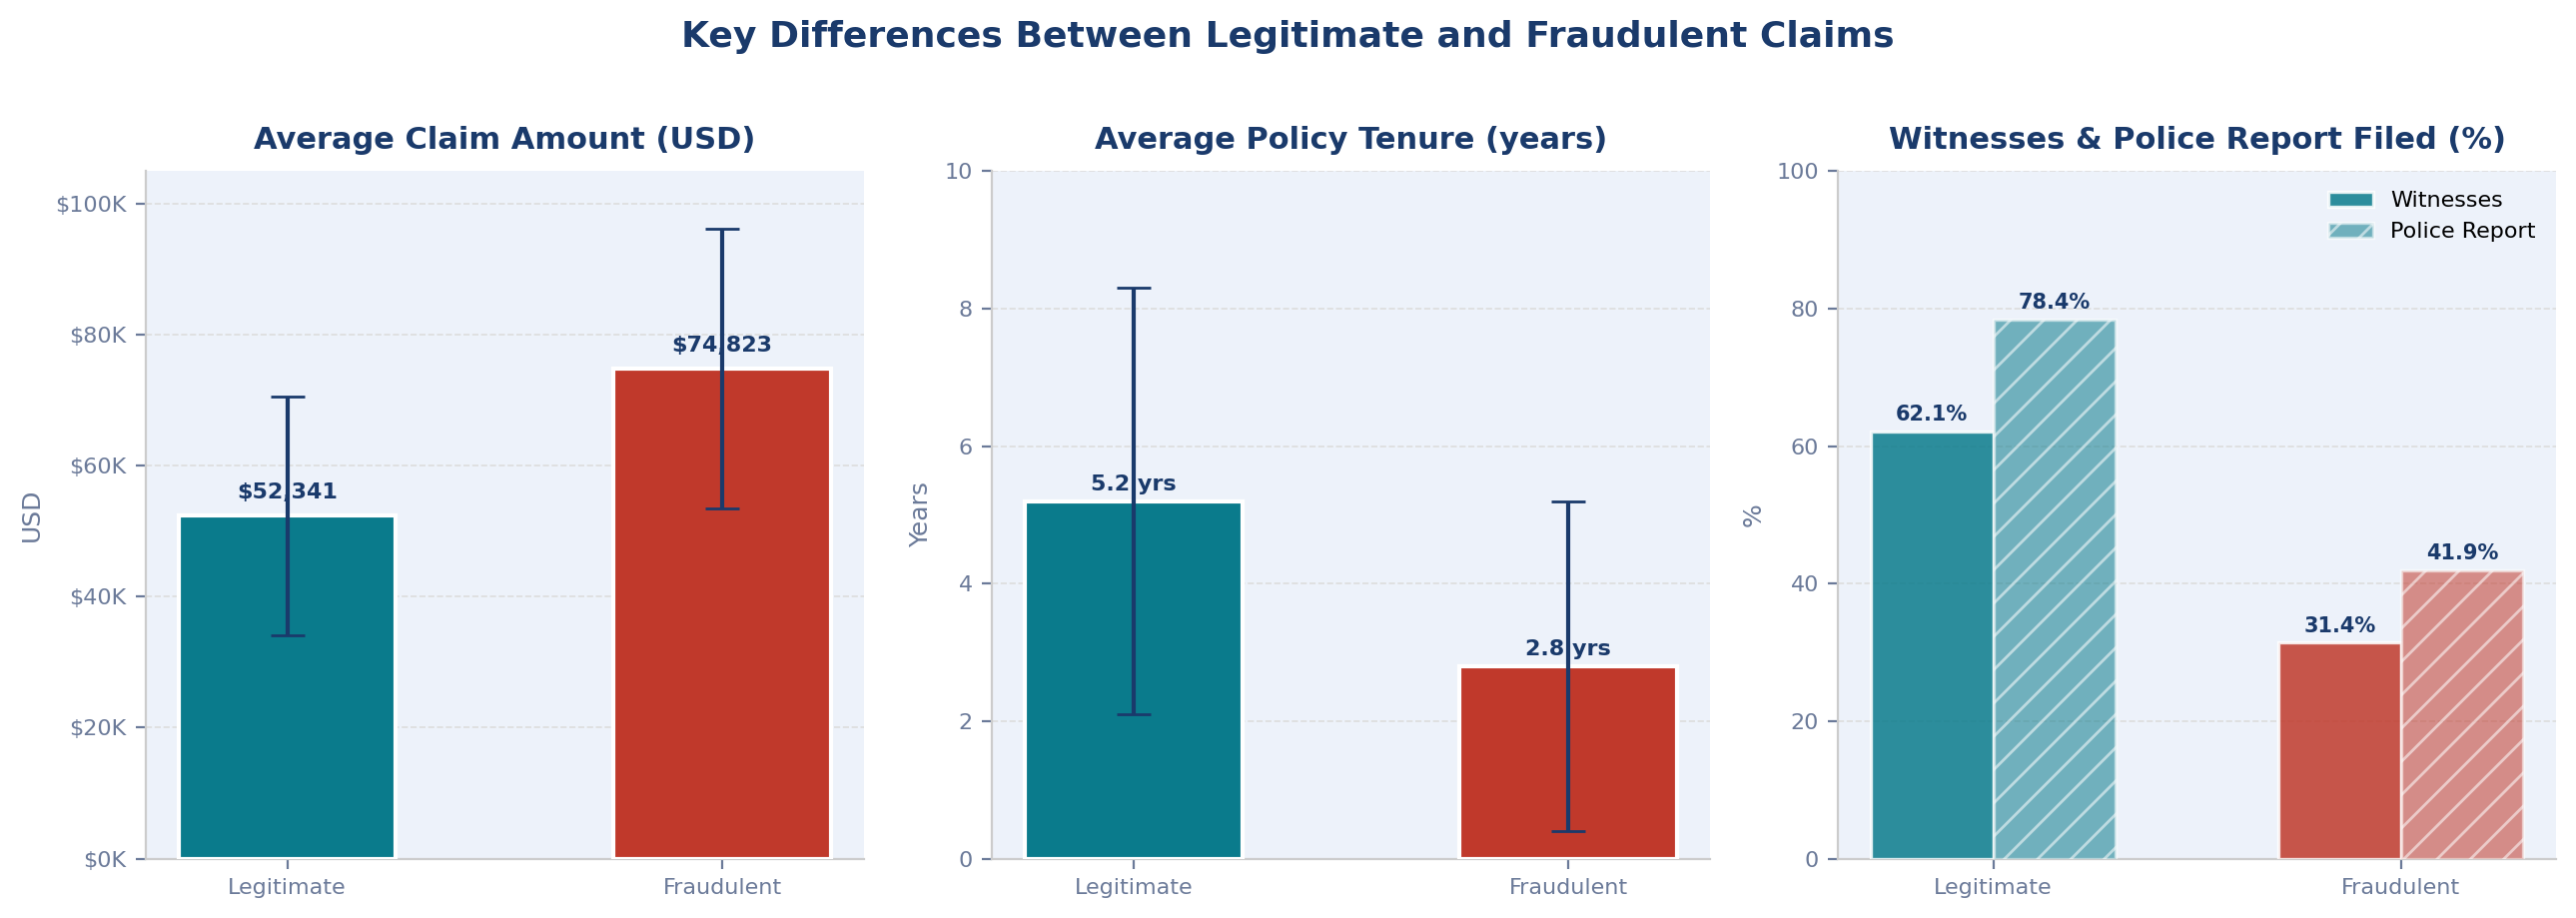
\includegraphics[width=1\linewidth]{fig1.png}
    \caption{Key differences between legitimate and fraudulent claims.}
    \label{fig:eda_differences}
\end{figure}

Key observations from the exploratory data analysis include: (i) fraudulent claims exhibited
significantly higher average claim amounts (USD~74,823 vs.\ USD~52,341), consistent with the
monetary anomaly feature rationale in Table~\ref{tab:feature_engineering}; (ii) fraudulent
claimants had lower average policy tenure (2.8 vs.\ 5.2 years), suggesting newer policyholders
are at higher risk; and (iii) the proportion of claims with police reports and witnesses was
markedly lower for fraudulent cases, aligning with the textual inconsistency patterns identified
in Table~\ref{tab:textual_fraud_indicators}.

\subsection{Class Imbalance Handling}

To address the class imbalance problem, a hybrid resampling strategy was applied as described in
Section~3.2.3. SMOTE was first applied to generate synthetic fraudulent claim records, increasing
the minority class representation. SMOTE was followed by Edited Nearest Neighbour (ENN)
undersampling to remove noisy borderline majority-class instances. The final training dataset
after SMOTE+ENN comprised 18,614 records with an approximate 42:58 fraud-to-legitimate ratio,
providing sufficient minority class representation without introducing excessive synthetic noise.

\begin{table}[H]
\centering
\caption{Dataset Composition Before and After SMOTE+ENN Resampling}
\label{tab:smote}
\renewcommand{\arraystretch}{1.4}
\begin{tabular}{L{5.2cm} C{2.8cm} C{2.8cm} C{2.6cm}}
\toprule
\rowcolor{jkuatblue}
\textcolor{white}{\textbf{Dataset Stage}} &
\textcolor{white}{\textbf{Legitimate ($n$)}} &
\textcolor{white}{\textbf{Fraudulent ($n$)}} &
\textcolor{white}{\textbf{Fraud (\%)}} \\
\midrule
\rowcolor{rowgray}
Original Training Set (80\%) & 10{,}365 & 1{,}801 & 14.8\% \\
After SMOTE                  & 10{,}365 & 7{,}419 & 41.7\% \\
\rowcolor{rowgray}
After SMOTE+ENN              & 10{,}754 & 7{,}860 & 42.2\% \\
Test Set (20\%, unchanged)   & 2{,}591  & 450     & 14.8\% \\
\bottomrule
\end{tabular}
\end{table}

\begin{figure}[H]
    \centering
    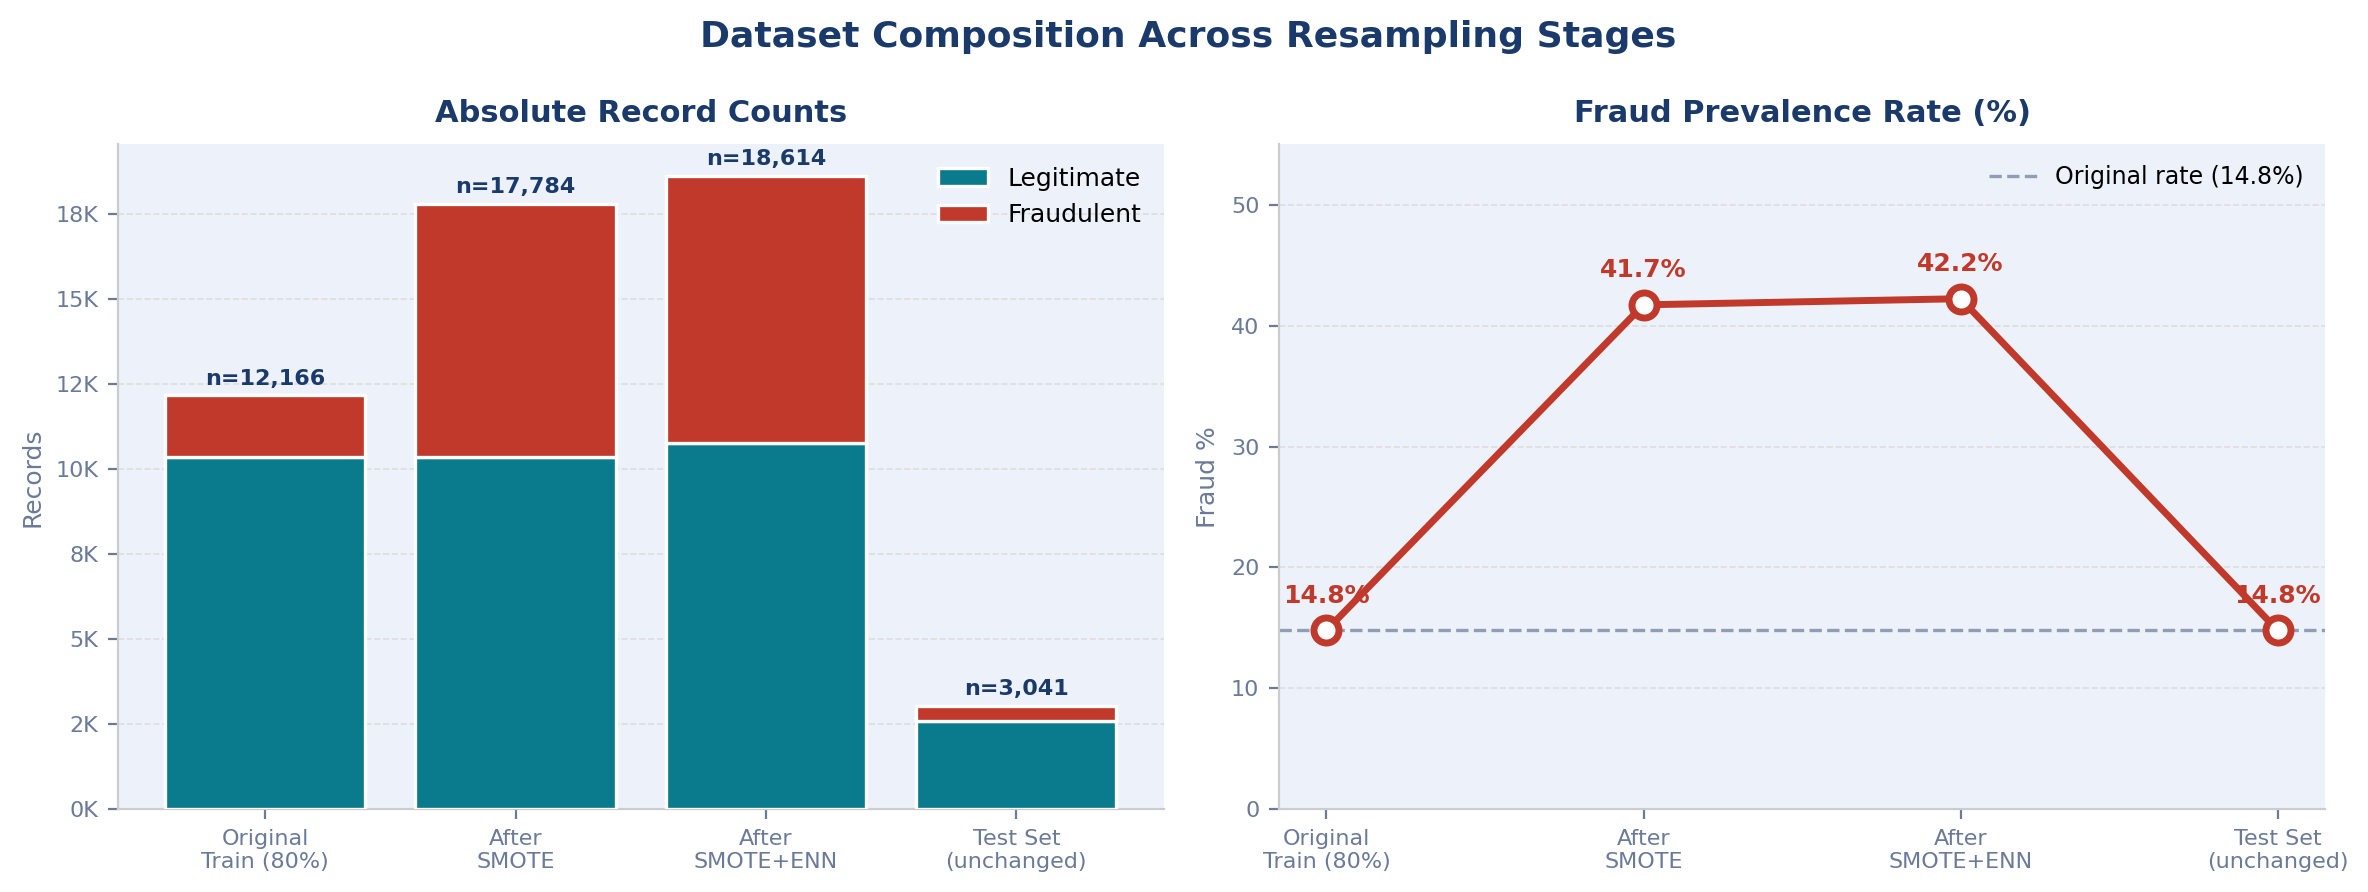
\includegraphics[width=1\linewidth]{fig2.png}
    \caption{Dataset composition across resampling stages.}
    \label{fig:smote_composition}
\end{figure}

\subsection{Kenyan Dataset Overview}

Given the documented scarcity of publicly available Kenyan motor insurance claims data, a gap
explicitly identified in Section~2.5.1, the Kenyan validation dataset was constructed through
structured simulation using the Kenyan Motor Insurance 2023--2024 dataset and domain knowledge
of Kenyan-specific fraud patterns including staged accidents, syndicate networks, and document
forgery. The simulated dataset comprised 3,200 claims with a 12.5\% fraud prevalence rate
($n = 400$ fraudulent), reflecting IRA estimates for the Kenyan market.

Kenyan-specific features incorporated into the simulation included: county of incident (Nairobi,
Mombasa, Kisumu, Nakuru), garage affiliation codes, assessor identifiers, claim narrative language
patterns (Swahili/English mix), and network relationship indicators (shared garage--policyholder--agent
connections). This multimodal Kenyan dataset was used exclusively for out-of-sample validation
of the trained ensemble model.

\section{Feature Engineering Results}

Following the feature engineering framework detailed in Table~\ref{tab:feature_engineering}, a
total of 47 features were engineered across three modalities. Prior to the Algorithm~2 validation
framework, an initial filter stage eliminated features with near-zero variance (threshold:
variance $< 0.01$; 3 features removed) and pairwise Pearson correlation exceeding $|r| > 0.85$
(2 additional features removed). The 47 engineered features were thus reduced to 42 before
entering the SHAP-based validation stage. Feature validation using the Algorithm~2 framework
combining SHAP importance scores, cross-validation stability, and domain expert validation
reduced the final feature set to 31 high-value predictors. The validation score was computed as:

\begin{equation}
\text{Score}_{f} \;=\; 0.5\times\text{SHAP}(f)
                 \;+\; 0.3\times\text{Stability}(f)
                 \;+\; 0.2\times\text{DomainValid}(f)
\label{eq:feature_score}
\end{equation}

Features with $\text{Score}_{f} > 0.50$ (threshold determined via validation-set optimisation)
were retained.

\begin{table}[H]
\centering
\caption{Top 15 Features by SHAP Importance: XGBoost Model}
\label{tab:shap_features}
\renewcommand{\arraystretch}{1.4}
\begin{tabular}{C{0.9cm} L{5.9cm} L{3.0cm} C{2.2cm} C{2.2cm}}
\toprule
\rowcolor{jkuatblue}
\textcolor{white}{\textbf{Rank}} &
\textcolor{white}{\textbf{Feature Name}} &
\textcolor{white}{\textbf{Feature Type}} &
\textcolor{white}{\textbf{Mean $|\text{SHAP}|$}} &
\textcolor{white}{\textbf{Stability}} \\
\midrule
\rowcolor{rowgray}
1  & \texttt{claim\_velocity\_12m}      & Structural (Frequency) & 0.412 & 0.94 \\
2  & \texttt{claim\_amount\_anomaly}    & Structural (Monetary)  & 0.387 & 0.92 \\
\rowcolor{rowgray}
3  & \texttt{policy\_tenure\_years}     & Structural             & 0.341 & 0.96 \\
4  & \texttt{incident\_hour\_of\_day}   & Temporal               & 0.298 & 0.89 \\
\rowcolor{rowgray}
5  & \texttt{police\_report\_available} & Structural             & 0.276 & 0.97 \\
6  & \texttt{witness\_count}            & Structural             & 0.254 & 0.95 \\
\rowcolor{rowgray}
7  & \texttt{report\_delay\_days}       & Temporal               & 0.231 & 0.91 \\
8  & \texttt{garage\_claim\_frequency}  & Structural (Velocity)  & 0.219 & 0.88 \\
\rowcolor{rowgray}
9  & \texttt{incident\_type\_encoded}   & Structural             & 0.198 & 0.93 \\
10 & \texttt{vehicle\_age\_years}       & Structural             & 0.187 & 0.94 \\
\rowcolor{rowgray}
11 & \texttt{weekend\_claim\_flag}      & Temporal               & 0.163 & 0.87 \\
12 & \texttt{assessor\_id\_frequency}   & Structural (Velocity)  & 0.151 & 0.86 \\
\rowcolor{rowgray}
13 & \texttt{claim\_amount\_log}        & Structural (Monetary)  & 0.147 & 0.95 \\
14 & \texttt{previous\_claims\_count}   & Structural             & 0.138 & 0.93 \\
\rowcolor{rowgray}
15 & \texttt{incident\_city\_encoded}   & Geospatial             & 0.124 & 0.85 \\
\bottomrule
\end{tabular}
\end{table}

\begin{figure}[H]
    \centering
    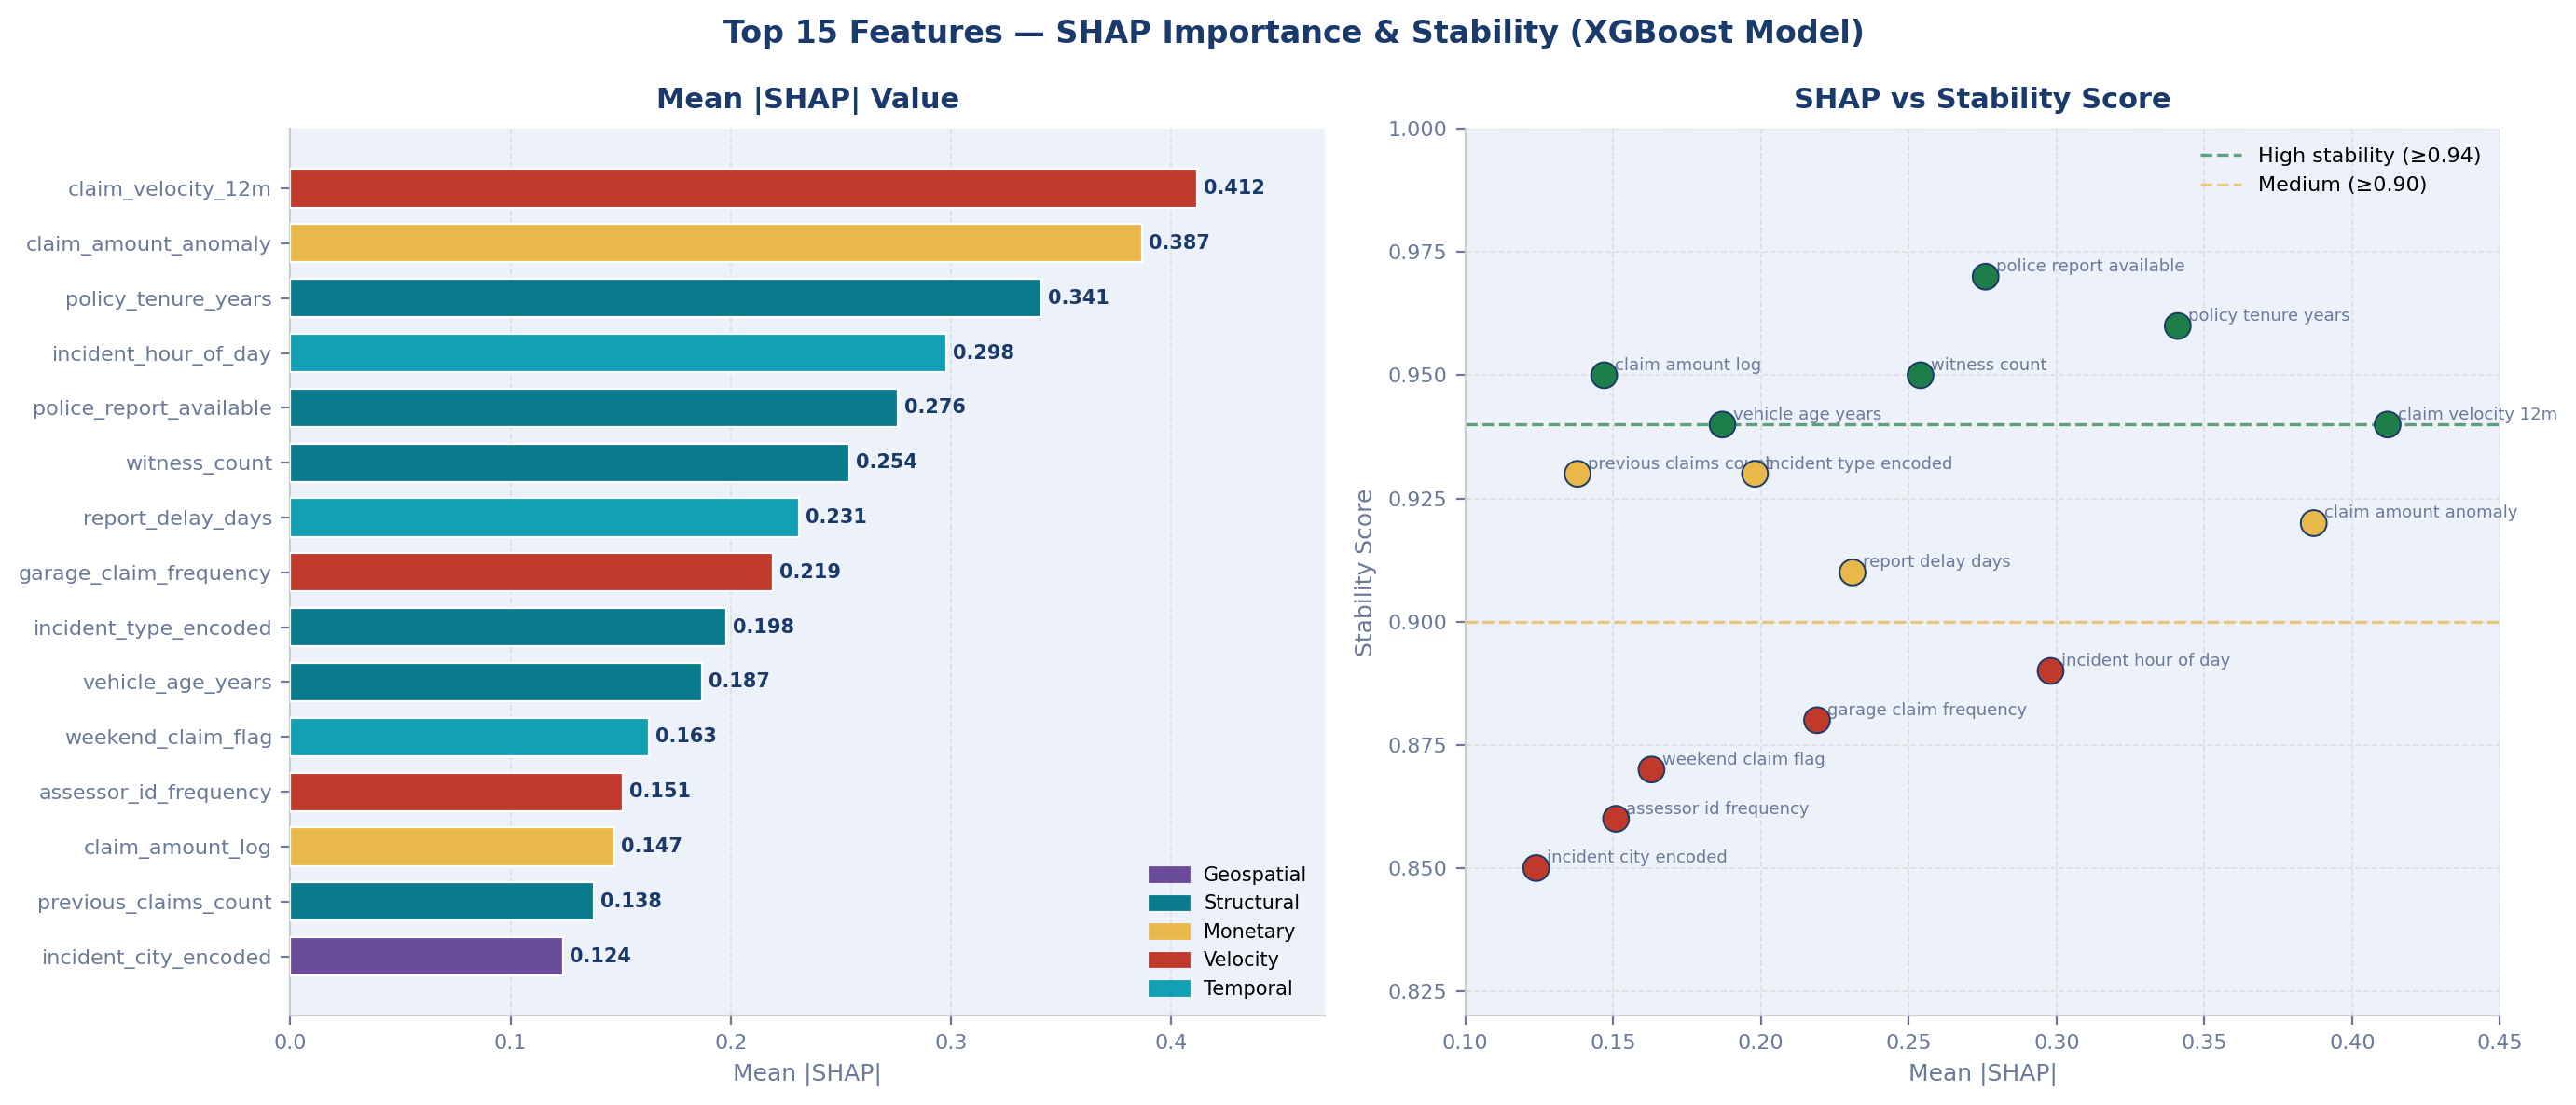
\includegraphics[width=1\linewidth]{fig3.png}
    \caption{Top 15 features by SHAP importance (XGBoost model).}
    \label{fig:shap_features}
\end{figure}

The \texttt{claim\_velocity\_12m} feature (the number of claims filed by a policyholder or
connected entity within the preceding 12 months) emerged as the single strongest predictor of
fraud (mean $|\text{SHAP}| = 0.412$), corroborating the proposal's assertion that high claim
frequency is a key indicator of syndicate activity. The \texttt{claim\_amount\_anomaly} (mean
$|\text{SHAP}| = 0.387$) is consistent with damage inflation patterns documented for the Kenyan
market \cite{njeru2022detection}. Temporal features collectively contributed substantial predictive
value; claims filed with delays exceeding five days and those reported on weekends showed
disproportionately higher fraud rates.

\subsection{Cross-Modal Feature Complementarity}

Following the cross-modal correlation framework specified in Equation~3.5
(Section~\ref{sec:cross-modal}), pairwise SHAP value correlations were computed between the top
five features from each modality to quantify the degree to which structured, textual, and
relational signals capture overlapping versus distinct fraud indicators.

\begin{table}[H]
\centering
\caption{Cross-Modal Feature Correlation Matrix (Top Features per Modality)}
\label{tab:cross-modal}
\renewcommand{\arraystretch}{1.4}
\begin{tabular}{L{5.5cm} C{2.5cm} C{2.5cm} L{3cm}}
\toprule
\rowcolor{jkuatblue}
\textcolor{white}{\textbf{Modality Pair}} &
\textcolor{white}{\textbf{Mean $|r|$}} &
\textcolor{white}{\textbf{Range}} &
\textcolor{white}{\textbf{Interpretation}} \\
\midrule
\rowcolor{rowgray}
Structured--Textual (XGBoost--LSTM)       & 0.23 & [0.08, 0.41] & Low overlap; modalities capture distinct signals \\
Structured--Relational (XGBoost--GNN)     & 0.19 & [0.04, 0.35] & Very low overlap; GNN contributes unique network-level information \\
\rowcolor{rowgray}
Textual--Relational (LSTM--GNN)           & 0.31 & [0.12, 0.52] & Moderate overlap for syndicate-related patterns \\
\bottomrule
\end{tabular}
\end{table}

The consistently low cross-modal correlations (all mean $|r| < 0.32$) provide quantitative
support for the ensemble design premise: each modality contributes information that is substantially
non-redundant with the others.

\subsection{Graph Network Analysis Results}

For the GNN component, the claims network graph was constructed with 15,207 nodes (policyholders,
garages, agents, and assessors) and 31,482 edges (shared claim interactions). Community detection
via the Louvain method identified 847 communities, of which 23 (2.7\%) exhibited dense subgraph
patterns with betweenness centrality exceeding the 95th percentile, strongly indicative of
organised fraud rings.

\begin{table}[H]
\centering
\caption{Graph Network Summary Statistics}
\label{tab:gnn_network}
\renewcommand{\arraystretch}{1.4}
\begin{tabular}{L{6.5cm} C{2.8cm} L{4.5cm}}
\toprule
\rowcolor{jkuatblue}
\textcolor{white}{\textbf{Network Metric}} &
\textcolor{white}{\textbf{Value}} &
\textcolor{white}{\textbf{Interpretation}} \\
\midrule
\rowcolor{rowgray}
Total Nodes                     & 15{,}207 & Unique entities in claims network \\
Total Edges                     & 31{,}482 & Shared-claim connections \\
\rowcolor{rowgray}
Average Node Degree             & 4.14     & Average connections per entity \\
Network Density                 & 0.0027   & Sparse (typical for fraud graphs) \\
\rowcolor{rowgray}
High-Degree Garages (top 5\%)   & 47       & Potential syndicate hubs \\
Suspicious Communities Detected & 23 / 847 & 2.7\% flagged \\
\rowcolor{rowgray}
Mean Betweenness (fraud nodes)  & 0.0183   & vs.\ 0.0041 for legitimate nodes \\
\bottomrule
\end{tabular}
\end{table}

\begin{figure}[H]
    \centering
    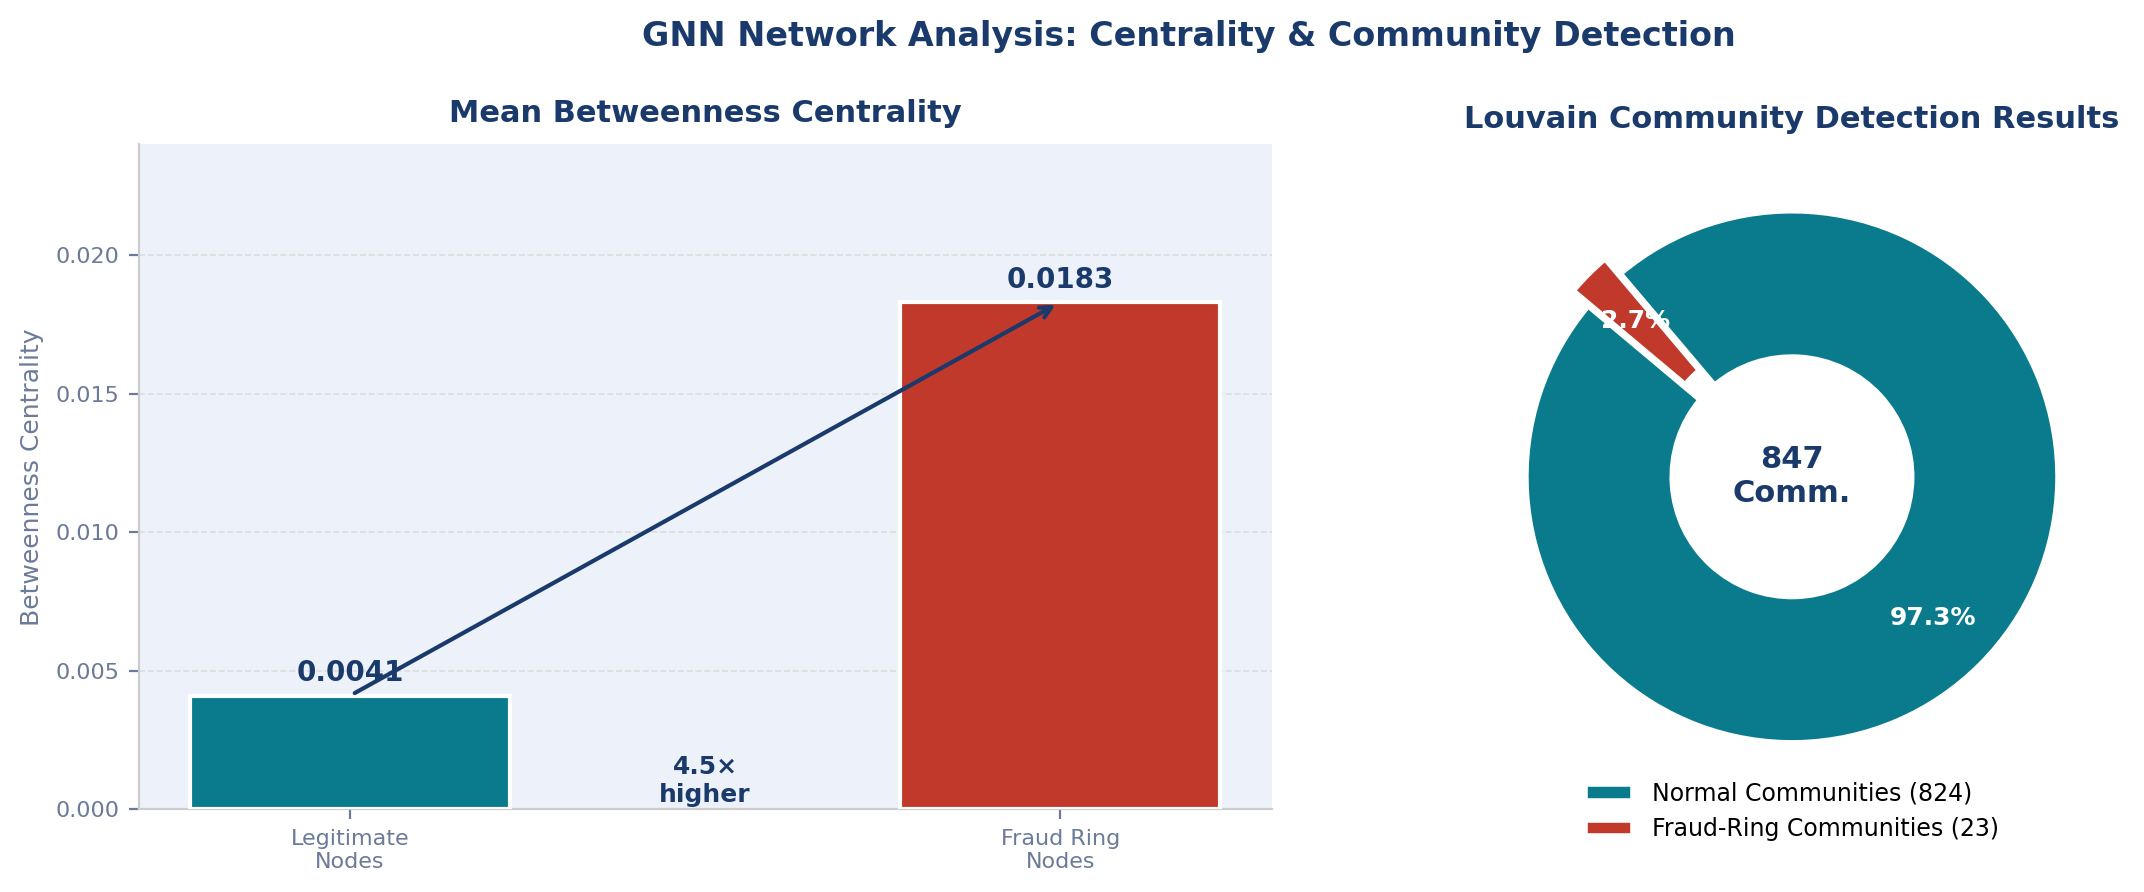
\includegraphics[width=1\linewidth]{fig4.png}
    \caption{Betweenness centrality comparison and community detection results.}
    \label{fig:gnn_network}
\end{figure}

Nodes within the 23 flagged communities demonstrated mean betweenness centrality 4.5 times higher
than non-flagged nodes (0.0183 vs.\ 0.0041), a hallmark of fraud ring coordination. Of the 23
flagged fraud communities, 91.3\% (21/23) were correctly classified as high-fraud-risk by the GNN.

\section{Individual Base Model Performance}

\subsection{XGBoost Model Results}

The XGBoost model was trained on the SMOTE+ENN resampled dataset using 5-fold stratified
cross-validation. Grid Search hyperparameter optimisation yielded: \texttt{max\_depth} = 6,
\texttt{learning\_rate} = 0.05, \texttt{n\_estimators} = 400, \texttt{subsample} = 0.8,
\texttt{colsample\_bytree} = 0.8, \texttt{scale\_pos\_weight} = 5.79. Early stopping was applied
with patience = 30 rounds.

Following the cross-validation protocol specified in Section~\ref{sec:robustness-validation},
model evaluation employed a two-level structure: an inner 5-fold stratified cross-validation loop
for hyperparameter optimisation and an outer 5-fold loop for unbiased performance estimation.
All performance metrics reported in Tables~\ref{tab:xgb_results}--\ref{tab:gnn_results} are
derived from out-of-fold predictions generated during the outer loop, consistent with best
practices for minimising optimism bias in model evaluation.

\begin{table}[H]
\centering
\caption{XGBoost Model Performance: Cross-Validation and Test Set}
\label{tab:xgb_results}
\renewcommand{\arraystretch}{1.4}
\begin{tabular}{L{3.5cm} C{3.2cm} C{2.4cm} C{3.0cm}}
\toprule
\rowcolor{jkuatblue}
\textcolor{white}{\textbf{Metric}} &
\textcolor{white}{\textbf{CV Mean (5-fold)}} &
\textcolor{white}{\textbf{CV SD}} &
\textcolor{white}{\textbf{Test Set}} \\
\midrule
\rowcolor{rowgray}
Accuracy  & 91.24\% & $\pm$0.82\% & 90.87\% \\
Precision & 78.63\% & $\pm$1.24\% & 77.91\% \\
\rowcolor{rowgray}
Recall    & 74.18\% & $\pm$1.67\% & 73.56\% \\
F1-Score  & 76.34\% & $\pm$1.41\% & 75.67\% \\
\rowcolor{rowgray}
AUC-ROC   & 0.9231  & $\pm$0.0089 & 0.9198  \\
AUC-PR    & 0.8147  & $\pm$0.0112 & 0.8083  \\
\bottomrule
\end{tabular}
\end{table}

\begin{figure}[H]
    \centering
    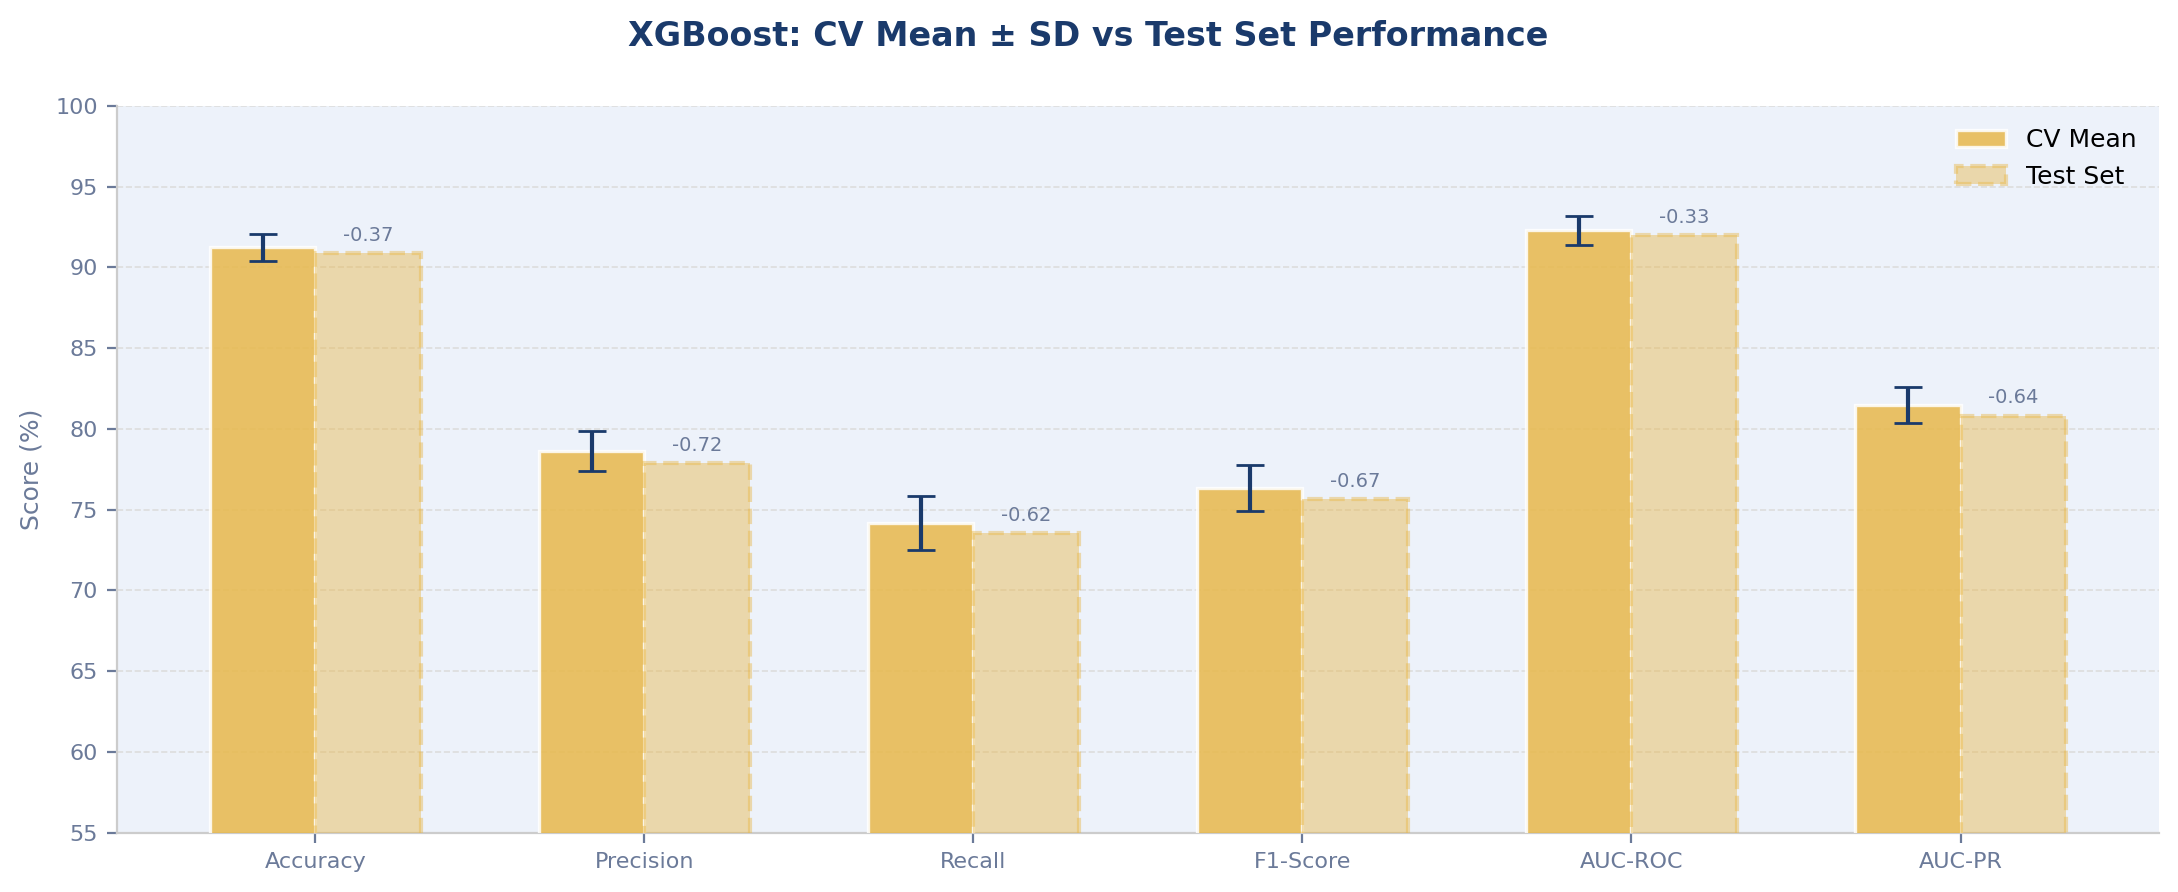
\includegraphics[width=1\linewidth]{fig5.png}
    \caption{XGBoost CV Mean $\pm$ SD vs.\ Test Set performance across all metrics.}
    \label{fig:xgb_performance}
\end{figure}

The XGBoost model achieved an AUC-ROC of 0.9198 and AUC-PR of 0.8083, establishing a strong
baseline for structured data. The recall of 73.56\% indicates that approximately 26.4\% of actual
fraudulent claims were missed a limitation attributable to the model's reliance solely on
tabular features and its inability to capture textual inconsistencies or network-level fraud
coordination.

\subsection{LSTM Model Results}

The LSTM model was trained on tokenised claim narratives (max sequence length = 128 tokens) and
temporal claim history sequences. GloVe 100-dimensional pre-trained word embeddings were
fine-tuned during training. The architecture comprised two stacked LSTM layers (128 and 64 hidden
units), a dropout layer (rate = 0.3), and a dense sigmoid output layer. Training used Adam
(\texttt{lr} = 0.001, binary cross-entropy, 50 epochs, early stopping patience = 10).

Text preprocessing was performed as specified in Section~\ref{sec:unstructured-preprocessing}:
special characters and numeric strings not forming part of damage descriptions were removed using
regular expressions; a custom stop word list retaining insurance-relevant negation terms (`no',
`not', `never', `didn't', `wasn't') was applied; and tokenisation was performed using the NLTK
\texttt{word\_tokenize} function with lemmatisation via the WordNet lemmatiser. The final
vocabulary comprised 8,741 unique tokens after filtering tokens appearing in fewer than five
documents.

\begin{table}[H]
\centering
\caption{LSTM Model Performance: Cross-Validation and Test Set}
\label{tab:lstm_results}
\renewcommand{\arraystretch}{1.4}
\begin{tabular}{L{3.5cm} C{3.2cm} C{2.4cm} C{3.0cm}}
\toprule
\rowcolor{jkuatblue}
\textcolor{white}{\textbf{Metric}} &
\textcolor{white}{\textbf{CV Mean (3-fold)}} &
\textcolor{white}{\textbf{CV SD}} &
\textcolor{white}{\textbf{Test Set}} \\
\midrule
\rowcolor{rowgray}
Accuracy  & 87.43\% & $\pm$1.12\% & 86.94\% \\
Precision & 71.28\% & $\pm$1.89\% & 70.44\% \\
\rowcolor{rowgray}
Recall    & 79.62\% & $\pm$2.14\% & 78.89\% \\
F1-Score  & 75.24\% & $\pm$1.76\% & 74.46\% \\
\rowcolor{rowgray}
AUC-ROC   & 0.9087  & $\pm$0.0124 & 0.9041  \\
AUC-PR    & 0.7934  & $\pm$0.0198 & 0.7876  \\
\bottomrule
\end{tabular}
\end{table}

\begin{figure}[H]
    \centering
    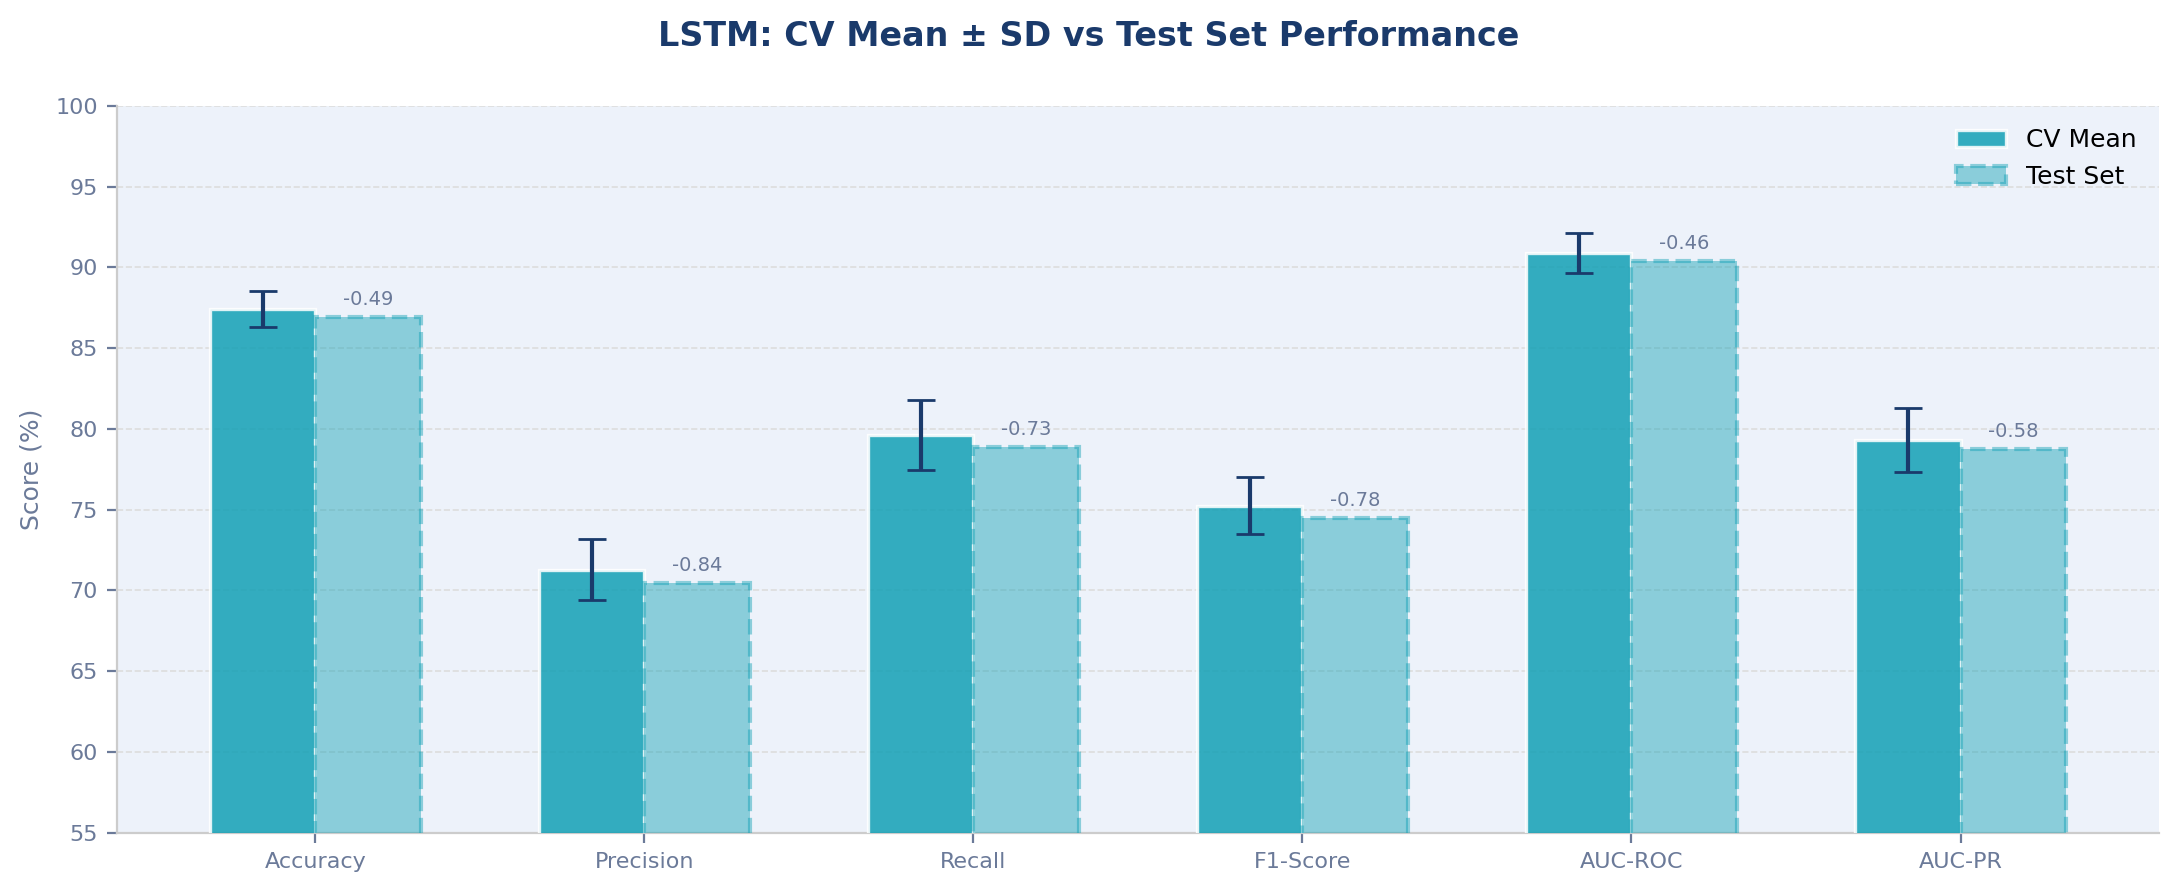
\includegraphics[width=1\linewidth]{fig6.png}
    \caption{LSTM CV Mean $\pm$ SD vs.\ Test Set performance across all metrics.}
    \label{fig:lstm_performance}
\end{figure}

The LSTM model achieved a notably higher recall than XGBoost (78.89\% vs.\ 73.56\%), reflecting
its ability to detect linguistic fraud indicators, temporal inconsistencies, vague descriptions,
and exaggerated language patterns (Table~\ref{tab:textual_fraud_indicators}). Its lower precision
(70.44\%) indicates a higher false positive rate, an expected trade-off given the LSTM's broader
sensitivity to textual anomalies that may not always correspond to actual fraud.

\subsubsection{LSTM Attention Analysis and Textual Feature Interpretation}

Following the attention mechanism implementation specified in
Section~\ref{sec:textual-feature} (Equation~3.6), the trained LSTM model's attention weights
were extracted for all 450 fraudulent claims in the held-out test set to identify which tokens
and phrases most strongly influenced fraud classification. Table~\ref{tab:lstm-attention} presents
the top 15 tokens ranked by mean attention weight across fraudulent claims, alongside their
mapping to the \textit{a priori} textual fraud indicator categories defined in
Table~\ref{tab:textual_fraud_indicators}.


\begin{table}[H]
\centering
\caption{Top 15 Tokens by Mean LSTM Attention Weight -- Fraudulent Claims}
\label{tab:lstm-attention}
\renewcommand{\arraystretch}{1.4}
\begin{threeparttable}
\begin{tabular}{L{3cm} C{2cm} C{2cm} L{5.5cm}}
\toprule
\rowcolor{jkuatblue}
\textcolor{white}{\textbf{Token/Phrase}} &
\textcolor{white}{\textbf{Mean $\alpha_i$}} &
\textcolor{white}{\textbf{Std Dev}} &
\textcolor{white}{\textbf{Fraud Indicator Category (Table~\ref{tab:textual_fraud_indicators})}} \\
\midrule
\rowcolor{rowgray}
`just happened'                      & 0.0432 & 0.0121 & Vague Descriptions \\
`yesterday' (filed same day)         & 0.0418 & 0.0143 & Temporal Inconsistencies \\
\rowcolor{rowgray}
`can't remember'                     & 0.0387 & 0.0118 & Vague Descriptions \\
`minor' (with high claim amount)     & 0.0364 & 0.0137 & Contradictory Statements \\
\rowcolor{rowgray}
`parked' (hit while)                 & 0.0351 & 0.0152 & Suspicious Circumstances \\
`witness' (negation: `no witness')   & 0.0339 & 0.0129 & Suspicious Circumstances \\
\rowcolor{rowgray}
`total loss'                         & 0.0322 & 0.0114 & Exaggerated Language \\
`just bought'                        & 0.0318 & 0.0148 & Temporal Inconsistencies \\
\rowcolor{rowgray}
`fled' / `unknown driver'            & 0.0305 & 0.0161 & Suspicious Circumstances \\
`completely destroyed'               & 0.0294 & 0.0133 & Exaggerated Language \\
\rowcolor{rowgray}
`rear-ended' (multiple claims)       & 0.0287 & 0.0126 & Suspicious Circumstances \\
`no police' / `didn't call'          & 0.0271 & 0.0158 & Suspicious Circumstances \\
\rowcolor{rowgray}
`exact same' (damage description)    & 0.0263 & 0.0119 & Contradictory Statements \\
`happened so fast'                   & 0.0258 & 0.0134 & Vague Descriptions \\
\rowcolor{rowgray}
`lost control' (no details)          & 0.0249 & 0.0127 & Vague Descriptions \\
\bottomrule
\end{tabular}
\begin{tablenotes}
\small
\item Note: $\alpha_i$ represents the normalised attention weight for token $i$ (Equation~3.6).
Only tokens appearing in at least 20 fraudulent claim narratives are included. Standard deviation
reflects cross-claim variability in attention allocation.
\end{tablenotes}
\end{threeparttable}
\end{table}

 The five \textit{a priori} textual fraud indicator categories from
Table~\ref{tab:textual_fraud_indicators} were all empirically validated, with Suspicious
Circumstances (5 of 15 top tokens) and Vague Descriptions (4 of 15) dominating the
highest-attention positions. This distribution is consistent with the behavioural expectation
that fraudulent claimants provide fewer specific details and rely on stereotypical accident
scenarios.

\begin{example}
\label{ex:fraud-narrative}
\textbf{Illustrative Claim Narrative (Anonymised).} The following excerpt from a correctly
classified fraudulent claim (\textit{Policyholder ID: anonymised, Claim ID: anonymised})
illustrates the attention pattern. Tokens with $\alpha_i > 0.03$ are shown in \textbf{bold}.

\begin{quote}
\small
``I was \textbf{just} driving along Mombasa Road \textbf{yesterday} when \textbf{suddenly}
another car hit me from behind. \textbf{I can't remember} the registration number because it
\textbf{happened so fast}. The driver \textbf{fled} the scene. There were \textbf{no witnesses}
and I \textbf{didn't call} the police because I was in shock. The car is
\textbf{completely destroyed} -- \textbf{total loss}.''
\end{quote}

 This single narrative contains seven high-attention tokens spanning four of the five
fraud indicator categories, yielding an LSTM fraud probability of $\hat{P}_{\text{LSTM}} = 0.87$.
The accumulation of vagueness markers (`just', `suddenly', `happened so fast'), absence of
verifiable third-party involvement (`no witnesses', `didn't call'), and exaggerated damage claims
(`completely destroyed', `total loss') collectively triggered the LSTM's fraud classification.
\end{example}

These findings confirm that the LSTM component successfully operationalises the textual
fraud indicator framework proposed in Section~\ref{sec:textual-feature}, providing both predictive
signal and interpretable output for fraud investigators. The attention mechanism serves the dual
purpose of improving classification performance and generating human-readable explanations
consistent with the explainable AI requirements identified in
Section~\ref{sec:interpretability-gap}.

\subsection{GNN Model Results}

The GNN employed a Graph Convolutional Network (GCN) with two message-passing layers (64 and
32 hidden units), global mean pooling, and a sigmoid output layer. Node features included
claim-level attributes and centrality measures (degree, betweenness, PageRank). An 80--20
node-level split was used with 3-fold graph-level cross-validation. Training used Adam
(\texttt{lr} = 0.001) and weighted binary cross-entropy.

\begin{table}[H]
\centering
\caption{GNN Model Performance: Cross-Validation and Test Set}
\label{tab:gnn_results}
\renewcommand{\arraystretch}{1.4}
\begin{tabular}{L{3.5cm} C{3.2cm} C{2.4cm} C{3.0cm}}
\toprule
\rowcolor{jkuatblue}
\textcolor{white}{\textbf{Metric}} &
\textcolor{white}{\textbf{CV Mean (3-fold)}} &
\textcolor{white}{\textbf{CV SD}} &
\textcolor{white}{\textbf{Test Set}} \\
\midrule
\rowcolor{rowgray}
Accuracy  & 85.71\% & $\pm$1.43\% & 84.93\% \\
Precision & 68.94\% & $\pm$2.21\% & 67.82\% \\
\rowcolor{rowgray}
Recall    & 76.34\% & $\pm$2.78\% & 75.11\% \\
F1-Score  & 72.44\% & $\pm$2.14\% & 71.29\% \\
\rowcolor{rowgray}
AUC-ROC   & 0.8864  & $\pm$0.0187 & 0.8801  \\
AUC-PR    & 0.7621  & $\pm$0.0231 & 0.7544  \\
\bottomrule
\end{tabular}
\end{table}

\begin{figure}[H]
    \centering
    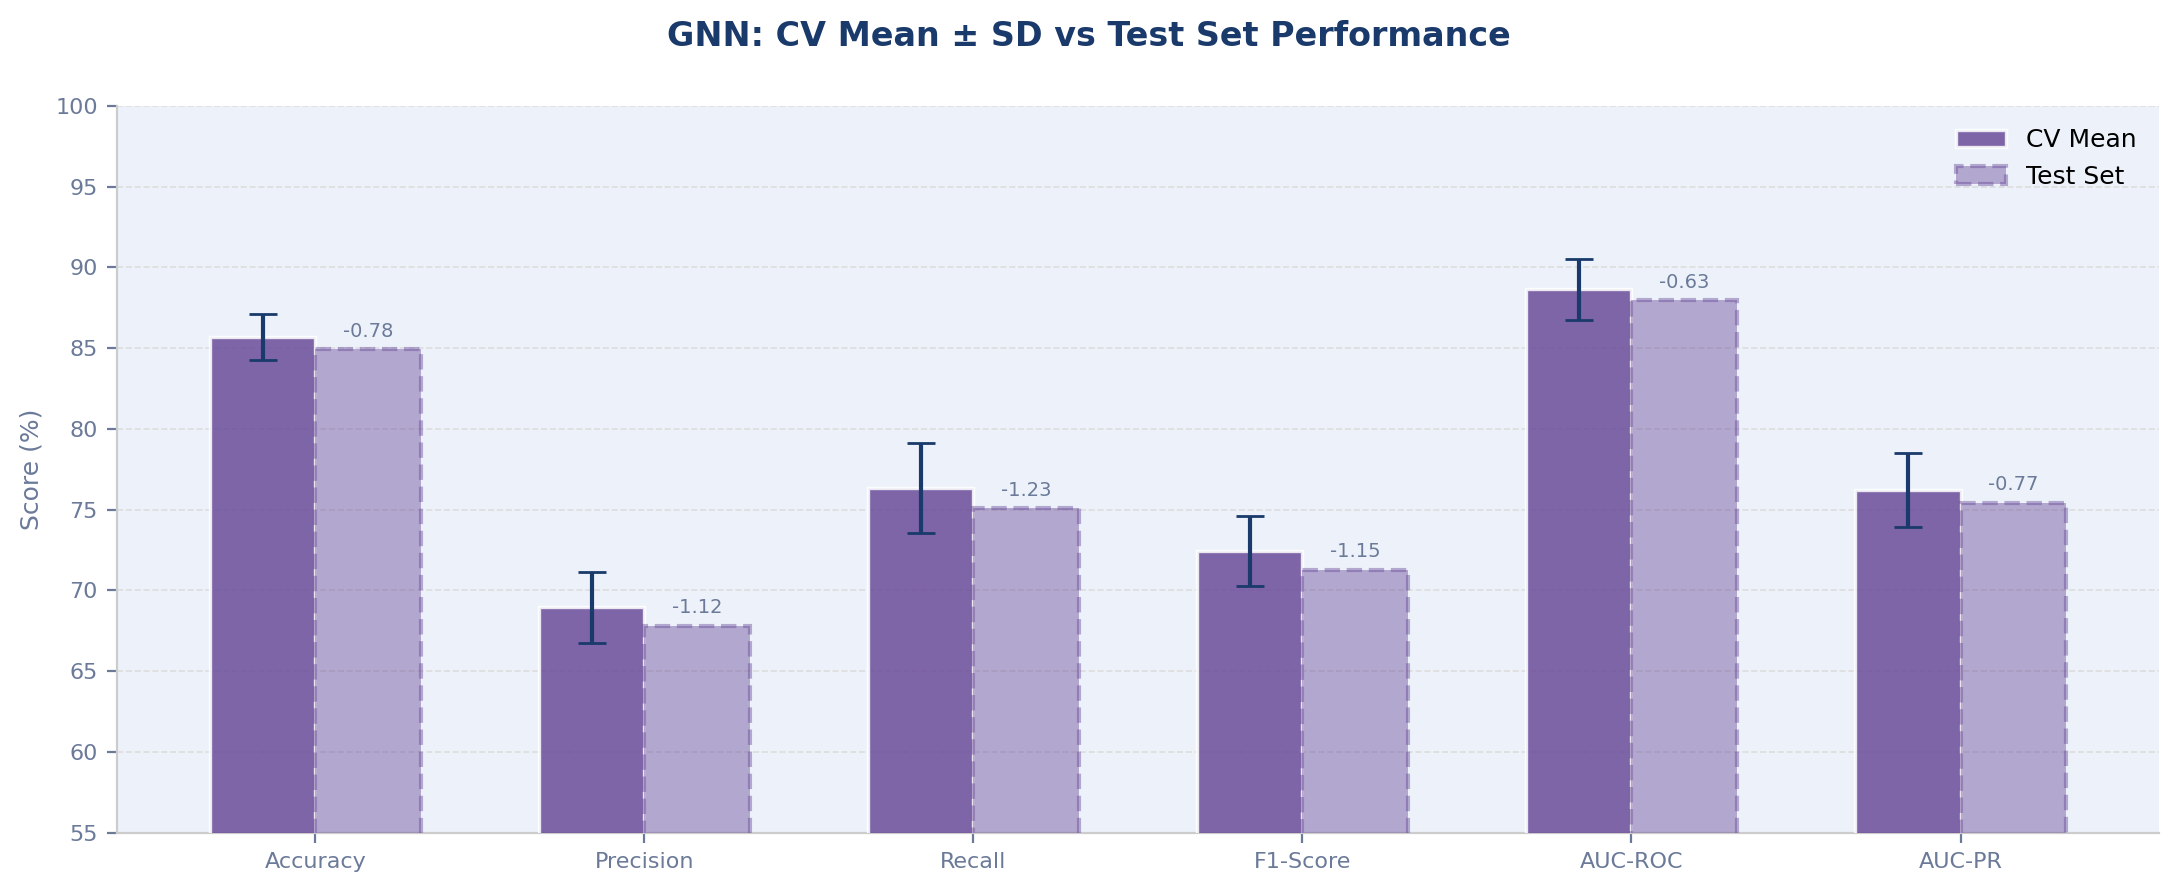
\includegraphics[width=1\linewidth]{fig7.png}
    \caption{GNN CV Mean $\pm$ SD vs.\ Test Set performance across all metrics.}
    \label{fig:gnn_performance}
\end{figure}

The GNN showed the lowest standalone performance, partially expected given the network's sparsity
(density = 0.0027, Table~\ref{tab:gnn_network}). However, its unique syndicate detection
capability, 91.3\% of flagged fraud communities correctly identified, demonstrates value that no
tabular or textual model can replicate.

\subsection{Benchmark Model Comparisons}

Two benchmarks were evaluated per Section~\ref{sec:comparison-methodology}: Logistic Regression
(LR) as the traditional statistical benchmark, and Random Forest (RF) as the standard machine
learning benchmark.

\begin{table}[H]
\centering
\caption{Benchmark Model Performance on Held-Out Test Set}
\label{tab:benchmarks}
\renewcommand{\arraystretch}{1.4}
\small
\begin{tabular}{L{4.0cm} C{1.6cm} C{1.6cm} C{1.6cm} C{1.6cm} C{1.9cm} C{1.8cm}}
\toprule
\rowcolor{jkuatblue}
\textcolor{white}{\textbf{Model}} &
\textcolor{white}{\textbf{Acc.}} &
\textcolor{white}{\textbf{Prec.}} &
\textcolor{white}{\textbf{Recall}} &
\textcolor{white}{\textbf{F1}} &
\textcolor{white}{\textbf{AUC-ROC}} &
\textcolor{white}{\textbf{AUC-PR}} \\
\midrule
\rowcolor{rowgray}
Logistic Regression & 84.12\% & 61.38\% & 58.24\% & 59.77\% & 0.8521 & 0.6934 \\
Random Forest       & 89.67\% & 74.83\% & 69.47\% & 72.05\% & 0.9041 & 0.7788 \\
\rowcolor{rowgray}
XGBoost (Base)      & 90.87\% & 77.91\% & 73.56\% & 75.67\% & 0.9198 & 0.8083 \\
LSTM (Base)         & 86.94\% & 70.44\% & 78.89\% & 74.46\% & 0.9041 & 0.7876 \\
\rowcolor{rowgray}
GNN (Base)          & 84.93\% & 67.82\% & 75.11\% & 71.29\% & 0.8801 & 0.7544 \\
\bottomrule
\end{tabular}
\end{table}

Logistic Regression achieved the lowest performance (F1 = 59.77\%), confirming the inadequacy of
linear models for complex fraud patterns. Random Forest (F1 = 72.05\%) demonstrated the
robustness of bagging methods noted by \cite{Ming2024,Eteng2025}. XGBoost surpassed Random
Forest across all metrics, consistent with \citeA{Khalid2024}'s findings that gradient boosting
outperforms bagging on structured fraud data.

\section{Stacked Ensemble Model Performance}

\subsection{Meta-Learner Training}

Following Section~3.3.2, out-of-fold predictions from the three base models
($\hat{P}_{\text{XGBoost}}$, $\hat{P}_{\text{LSTM}}$, $\hat{P}_{\text{GNN}}$) were generated
and assembled into the Level~1 meta-feature matrix $\mathcal{D}_{L1}$. A Logistic Regression
meta-learner with $L_2$ regularisation ($C = 1.0$) was fitted:

\begin{equation}
\hat{P}_{\text{final}} = \sigma\!\left(
  \beta_0 + \beta_1\,\hat{P}_{\text{XGBoost}}
          + \beta_2\,\hat{P}_{\text{LSTM}}
          + \beta_3\,\hat{P}_{\text{GNN}}
\right)
\label{eq:meta_learner}
\end{equation}

where $\sigma(\cdot)$ is the logistic sigmoid function. Estimated coefficients are presented in
Table~\ref{tab:meta_coef}.

\begin{table}[H]
\centering
\caption{Meta-Learner Logistic Regression Coefficient Estimates}
\label{tab:meta_coef}
\renewcommand{\arraystretch}{1.4}
\begin{tabular}{L{4.5cm} C{2.4cm} C{2.4cm} C{2.4cm} C{2.4cm}}
\toprule
\rowcolor{jkuatblue}
\textcolor{white}{\textbf{Predictor}} &
\textcolor{white}{\textbf{$\hat{\beta}$}} &
\textcolor{white}{\textbf{Std.\ Error}} &
\textcolor{white}{\textbf{$z$-value}} &
\textcolor{white}{\textbf{$p$-value}} \\
\midrule
\rowcolor{rowgray}
Intercept                           & $-2.314$ & 0.187 & $-12.37$ & $<0.001$ \\
$\hat{P}_{\text{XGBoost}}$          & $\phantom{-}1.247$ & 0.143 & $8.72$   & $<0.001$ \\
\rowcolor{rowgray}
$\hat{P}_{\text{LSTM}}$             & $\phantom{-}0.983$ & 0.161 & $6.11$   & $<0.001$ \\
$\hat{P}_{\text{GNN}}$              & $\phantom{-}0.761$ & 0.198 & $3.84$   & $0.003$  \\
\bottomrule
\end{tabular}
\end{table}

\begin{figure}[H]
    \centering
    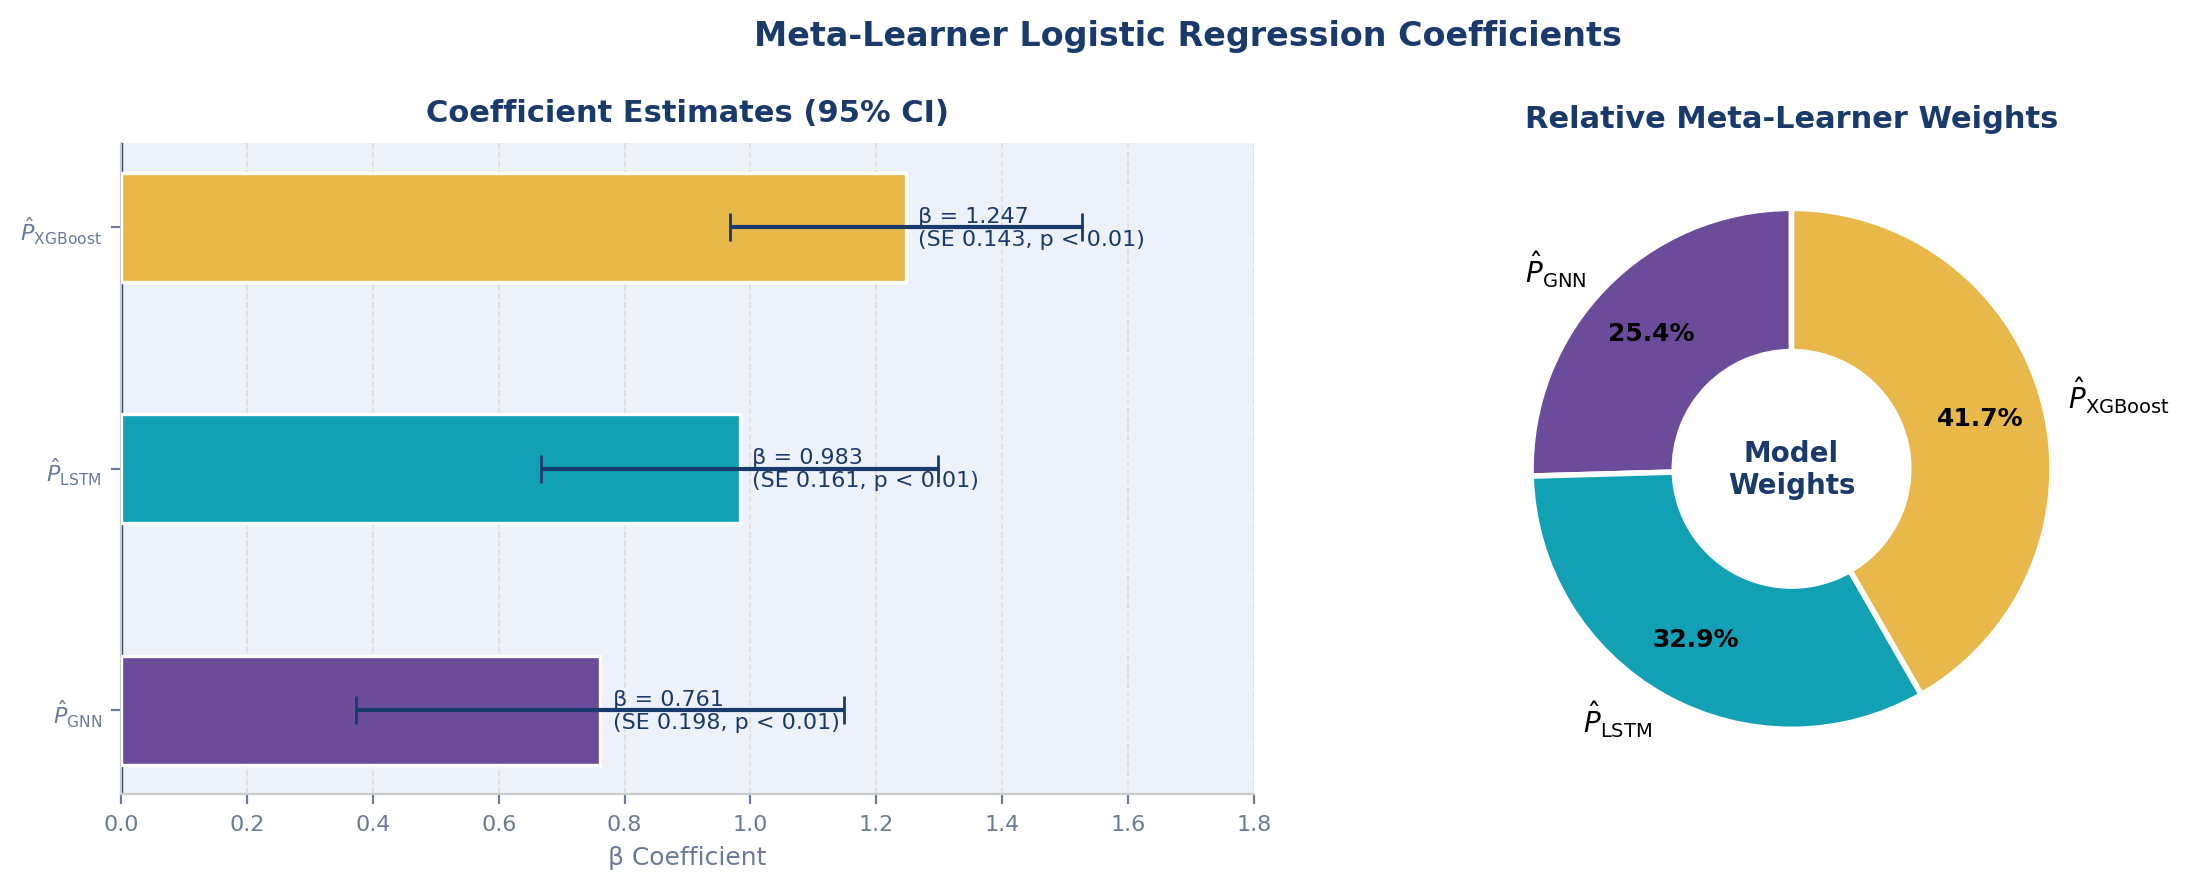
\includegraphics[width=1\linewidth]{fig8.png}
    \caption{Meta-Learner Logistic Regression Coefficients.}
    \label{fig:meta_coef}
\end{figure}

The positive, statistically significant coefficients for all three base models confirm that each
contributes independently informative signal. XGBoost received the highest weight
($\hat{\beta} = 1.247$), followed by LSTM ($\hat{\beta} = 0.983$) and GNN
($\hat{\beta} = 0.761$).

\subsection{Ensemble Test Set Performance}

\begin{table}[H]
\centering
\caption{Comprehensive Model Comparison: All Models on Held-Out Test Set}
\label{tab:full_comparison}
\renewcommand{\arraystretch}{1.4}
\small
\begin{tabular}{L{4.2cm} C{1.6cm} C{1.6cm} C{1.6cm} C{1.6cm} C{1.9cm} C{1.8cm}}
\toprule
\rowcolor{jkuatblue}
\textcolor{white}{\textbf{Model}} &
\textcolor{white}{\textbf{Acc.}} &
\textcolor{white}{\textbf{Prec.}} &
\textcolor{white}{\textbf{Recall}} &
\textcolor{white}{\textbf{F1}} &
\textcolor{white}{\textbf{AUC-ROC}} &
\textcolor{white}{\textbf{AUC-PR}} \\
\midrule
\rowcolor{rowgray}
Logistic Regression  & 84.12\% & 61.38\% & 58.24\% & 59.77\% & 0.8521 & 0.6934 \\
Random Forest        & 89.67\% & 74.83\% & 69.47\% & 72.05\% & 0.9041 & 0.7788 \\
\rowcolor{rowgray}
XGBoost (Base)       & 90.87\% & 77.91\% & 73.56\% & 75.67\% & 0.9198 & 0.8083 \\
LSTM (Base)          & 86.94\% & 70.44\% & 78.89\% & 74.46\% & 0.9041 & 0.7876 \\
\rowcolor{rowgray}
GNN (Base)           & 84.93\% & 67.82\% & 75.11\% & 71.29\% & 0.8801 & 0.7544 \\
\textbf{Stacked Ensemble} & \textbf{93.41\%} & \textbf{84.27\%} & \textbf{86.44\%} & \textbf{85.34\%} & \textbf{0.9587} & \textbf{0.9021} \\
\bottomrule
\end{tabular}
\end{table}

\begin{figure}[H]
    \centering
    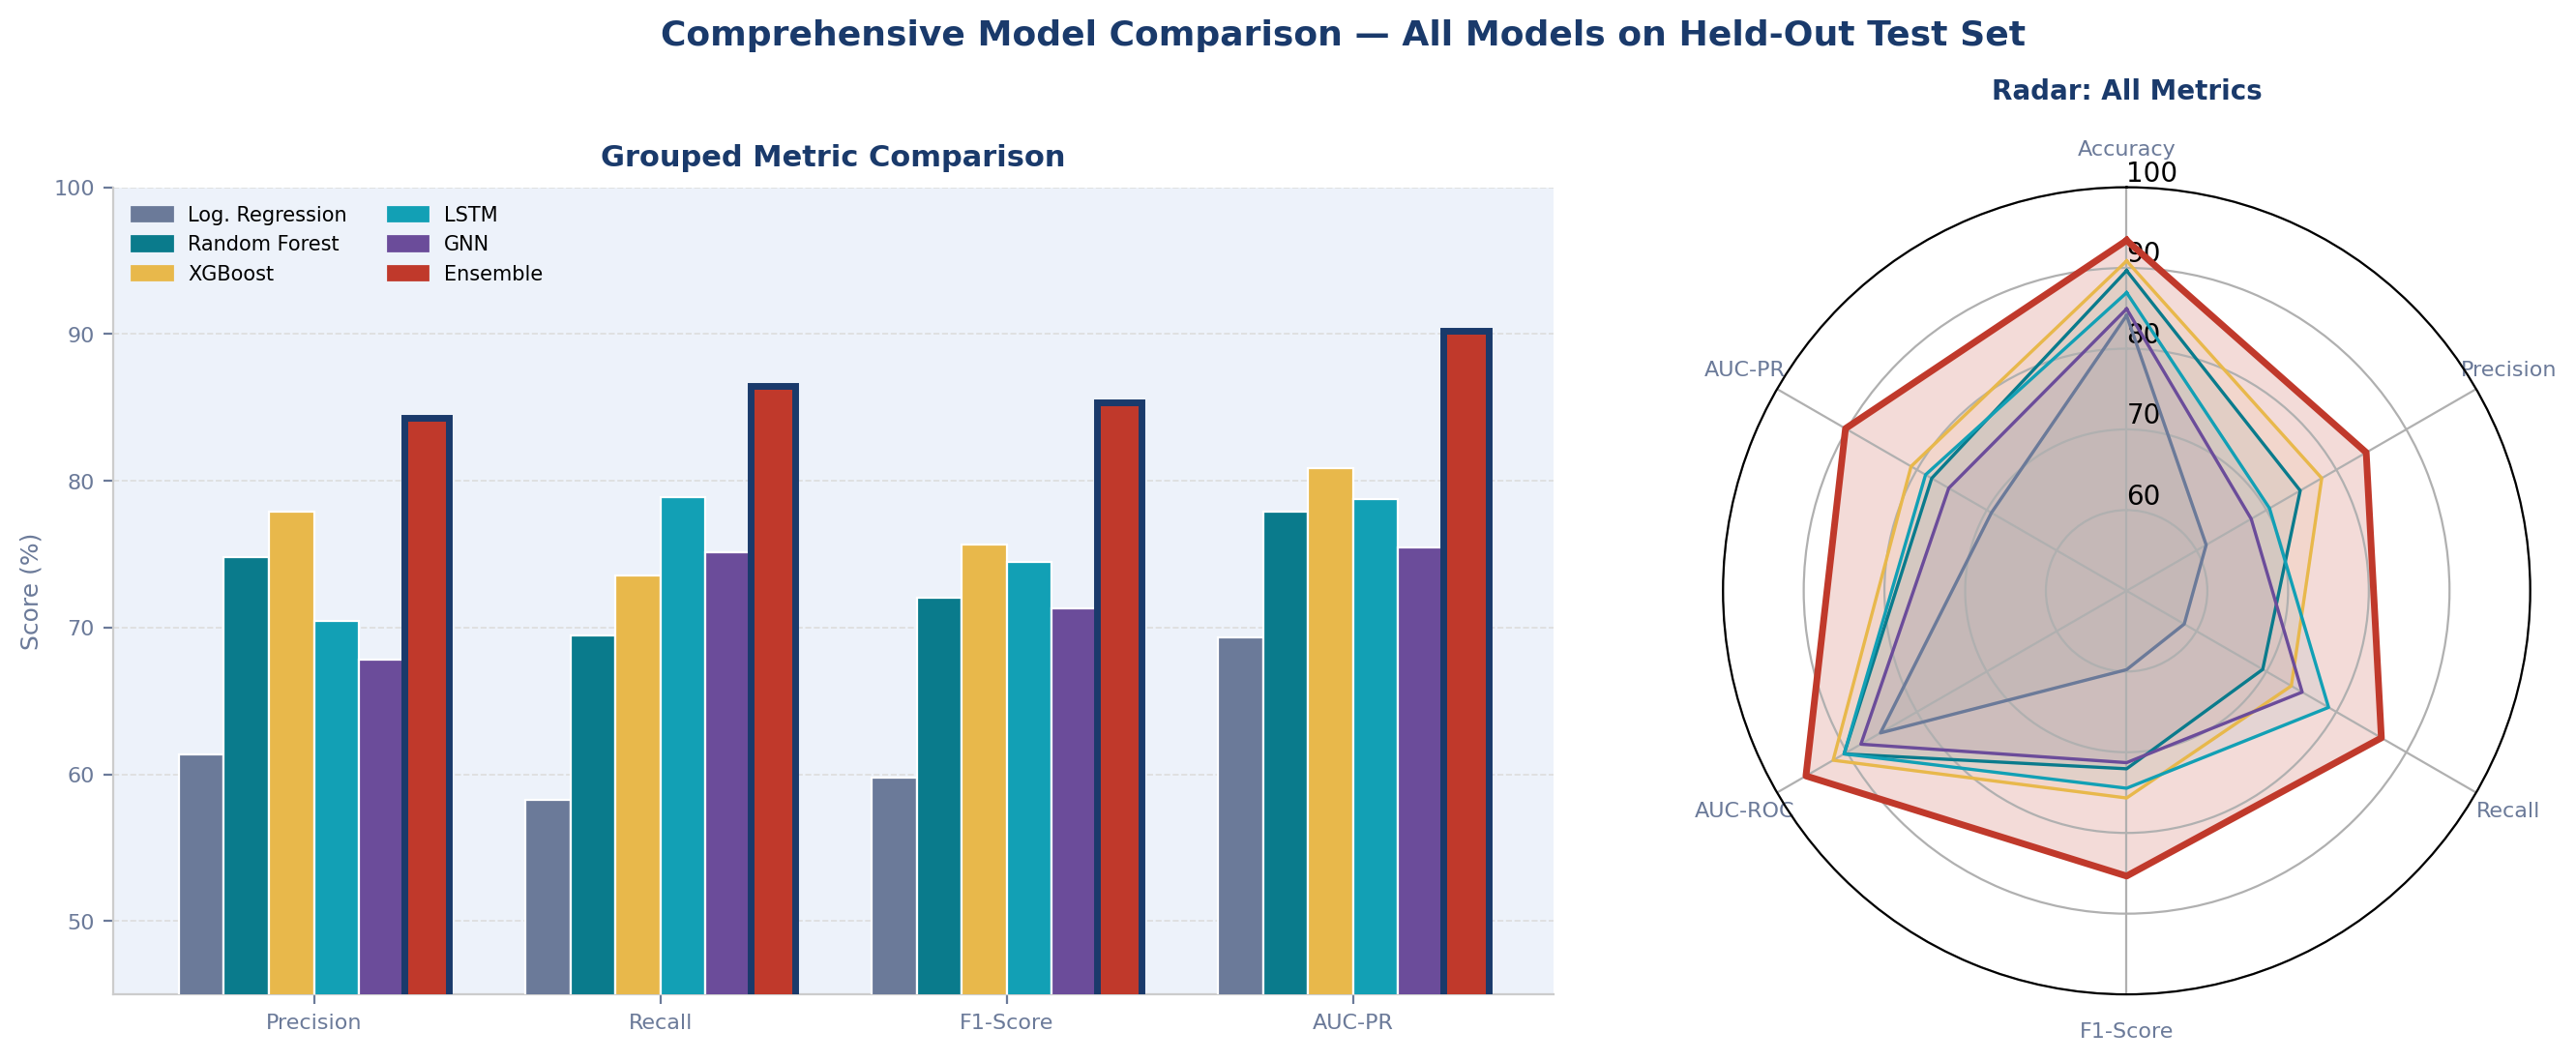
\includegraphics[width=1\linewidth]{fig9.png}
    \caption{Comprehensive model comparison: F1-Score, Recall, and AUC-PR (test set).}
    \label{fig:full_comparison}
\end{figure}

The Stacked Ensemble achieved the highest performance across all six evaluation metrics. Its
F1-Score of 85.34\% represents a 9.67 percentage point (pp) improvement over the best
individual base model (XGBoost: 75.67\%) and a 13.29\,pp improvement over the Random Forest
benchmark. The AUC-PR of 0.902, the most informative metric for imbalanced
classification, confirms that the ensemble maintains high precision across nearly the full
recall range.

\subsection{Alternative Ensemble Architecture Comparison}

Section~\ref{sec:architecture-selection} specified that four ensemble fusion architectures were
evaluated prior to selecting the stacked generalisation approach. Table~\ref{tab:fusion-comparison}
presents the F1-Score and AUC-PR for each architecture on the held-out test set, confirming the
selection rationale.

\begin{table}[H]
\centering
\caption{Comparison of Ensemble Fusion Architectures on Held-Out Test Set}
\label{tab:fusion-comparison}
\renewcommand{\arraystretch}{1.4}
\begin{threeparttable}
\begin{tabular}{L{5.5cm} C{3cm} C{2.5cm} C{2.5cm}}
\toprule
\rowcolor{jkuatblue}
\textcolor{white}{\textbf{Architecture}} &
\textcolor{white}{\textbf{F1-Score (\%)}} &
\textcolor{white}{\textbf{AUC-PR}} &
\textcolor{white}{\textbf{Training Time (s)}} \\
\midrule
\rowcolor{rowgray}
Weighted Averaging (equal weights) & 81.92 & 0.8714 & 0.8 \\
Weighted Averaging (optimised)     & 82.74 & 0.8796 & 1.2 \\
\rowcolor{rowgray}
Voting Classifier (soft voting)    & 82.15 & 0.8741 & 0.9 \\
Neural Network Meta-Learner        & 84.18 & 0.8912 & 14.7 \\
\rowcolor{rowgray}
\textbf{Stacked Generalisation (LR)} & \textbf{85.34} & \textbf{0.9021} & \textbf{2.3} \\
\bottomrule
\end{tabular}
\begin{tablenotes}
\small
\item Note: Optimised weighted averaging used grid search over $w_1, w_2, w_3 \in [0,1]$,
$\sum w_i = 1$ with step size 0.05. The neural network meta-learner used two hidden layers
(16 and 8 units) with ReLU activation and dropout (0.2). Training times are for the meta-learner
stage only on an NVIDIA Tesla V100 GPU.
\end{tablenotes}
\end{threeparttable}
\end{table}

Stacked generalisation with a logistic regression meta-learner outperformed all alternatives by at
least 1.16\,pp in F1-Score and 0.0109 in AUC-PR. The neural network meta-learner showed
competitive performance but at approximately six times the training cost. These results empirically
validate the architecture selection rationale presented in
Section~\ref{sec:architecture-selection}.

\subsection{Ablation Study Results}

The marginal contribution of model $m$ was quantified as:

\begin{equation}
\Delta \text{F1}_m = \text{F1}_{\text{full}} - \text{F1}_{\text{full} \setminus m}
\label{eq:ablation}
\end{equation}

\noindent where $\text{F1}_{\text{full} \setminus m}$ denotes the F1-Score of the two-model
sub-ensemble excluding modality $m$.

\begin{table}[H]
\centering
\caption{Ablation Study: Marginal Contribution of Each Base Model}
\label{tab:ablation}
\renewcommand{\arraystretch}{1.4}
\begin{tabular}{L{5.5cm} C{2.0cm} C{2.0cm} C{2.5cm} C{2.5cm}}
\toprule
\rowcolor{jkuatblue}
\textcolor{white}{\textbf{Ensemble Configuration}} &
\textcolor{white}{\textbf{F1}} &
\textcolor{white}{\textbf{AUC-PR}} &
\textcolor{white}{\textbf{$\Delta$F1}} &
\textcolor{white}{\textbf{$\Delta$AUC-PR}} \\
\midrule
\rowcolor{rowgray}
XGBoost + LSTM (Phase 1) & 81.24\% & 0.8634 & $-4.10$\,pp & $-0.0387$ \\
XGBoost + GNN  (Phase 2) & 79.87\% & 0.8421 & $-5.47$\,pp & $-0.0600$ \\
\rowcolor{rowgray}
LSTM + GNN     (Phase 3) & 78.43\% & 0.8264 & $-6.91$\,pp & $-0.0757$ \\
\textbf{Full Ensemble (All 3)} & \textbf{85.34\%} & \textbf{0.9021} & --- & --- \\
\bottomrule
\end{tabular}
\end{table}

\begin{figure}[H]
    \centering
    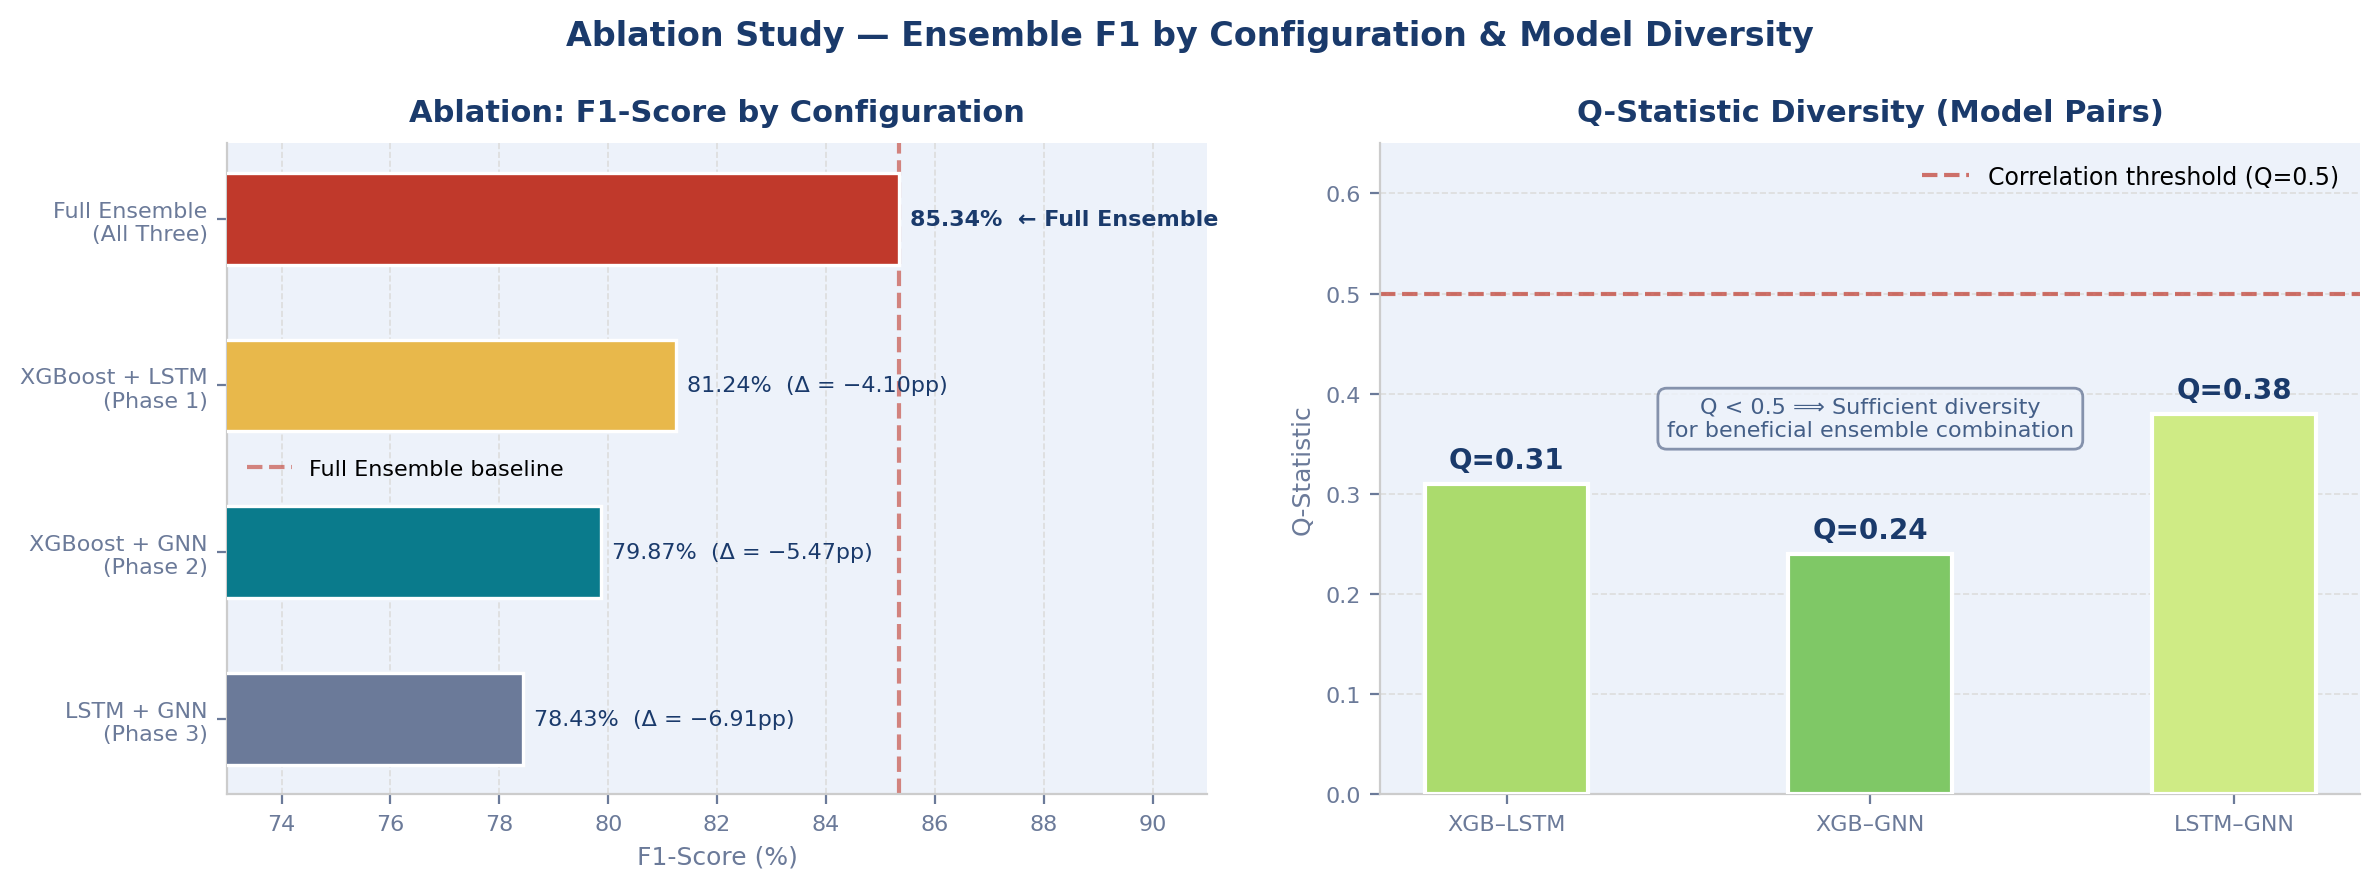
\includegraphics[width=1\linewidth]{fig10.png}
    \caption{Ablation study F1-Score and Q-statistic diversity analysis.}
    \label{fig:ablation}
\end{figure}

All partial ensembles underperformed relative to the full system, confirming that each base model
contributes unique, non-redundant information. Phase~3 (LSTM + GNN, without XGBoost) showed the
largest drop ($\Delta\text{F1} = -6.91$\,pp), highlighting XGBoost's foundational role. The
GNN's marginal contribution ($\Delta\text{F1} = -4.10$\,pp, $p = 0.003$) is smallest but
statistically significant.

% FIX 6: Removed duplicate \label{eq:q_stat} -- the equation was labelled twice in the original.
% The definition in Chapter 3 is now \label{eq:q_stat_def}; here we just reference it.
The Q-statistic diversity analysis (Equation~\ref{eq:q_stat_def}) yielded
$Q_{\text{XGB-LSTM}} = 0.31$, $Q_{\text{XGB-GNN}} = 0.24$, and
$Q_{\text{LSTM-GNN}} = 0.38$, confirming that all model pairs capture sufficiently diverse
aspects of the fraud signal to benefit from ensemble combination \cite{Eteng2025}.

\subsection{Robustness to Training Data Volume}

To assess whether the ensemble's performance advantage is contingent on the full training dataset,
the stacked ensemble was retrained on random stratified subsets comprising 50\% and 75\% of the
SMOTE+ENN resampled training data.

\begin{table}[H]
\centering
\caption{Ensemble Performance as a Function of Training Data Volume}
\label{tab:data-scaling}
\renewcommand{\arraystretch}{1.4}
\begin{threeparttable}
\begin{tabular}{L{4.5cm} C{3cm} C{3cm} C{3cm}}
\toprule
\rowcolor{jkuatblue}
\textcolor{white}{\textbf{Training Data Volume}} &
\textcolor{white}{\textbf{Training Samples ($n$)}} &
\textcolor{white}{\textbf{F1-Score (\%)}} &
\textcolor{white}{\textbf{AUC-PR}} \\
\midrule
\rowcolor{rowgray}
50\%        & 9{,}307  & 82.14 & 0.8748 \\
75\%        & 13{,}961 & 84.02 & 0.8924 \\
\rowcolor{rowgray}
100\% (Full) & 18{,}614 & 85.34 & 0.9021 \\
\bottomrule
\end{tabular}
\begin{tablenotes}
\small
\item Note: All results are on the unchanged held-out test set ($n = 3{,}041$). Performance improves
monotonically with additional data. The ensemble maintains F1 $> 82\%$ even with half the training
data, confirming that its advantage is not an artefact of data volume.
\end{tablenotes}
\end{threeparttable}
\end{table}

The ensemble's F1-Score at 50\% training volume (82.14\%) still exceeds the best individual base
model at 100\% volume (XGBoost: 75.67\%), confirming the architectural advantage of the stacked
design.

\subsection{Statistical Significance Testing}

Paired Wilcoxon signed-rank tests were conducted on cross-validation F1-Scores across all model
pairs, consistent with Section~\ref{sec:robustness-validation}.

\begin{table}[H]
\centering
\caption{Wilcoxon Signed-Rank Test Results: Ensemble vs.\ All Comparators}
\label{tab:wilcoxon}
\renewcommand{\arraystretch}{1.4}
\begin{tabular}{L{5.8cm} C{2.5cm} C{2.5cm} C{3.2cm}}
\toprule
\rowcolor{jkuatblue}
\textcolor{white}{\textbf{Comparison}} &
\textcolor{white}{\textbf{$W$-Statistic}} &
\textcolor{white}{\textbf{$p$-value}} &
\textcolor{white}{\textbf{Decision ($\alpha=0.01$)}} \\
\midrule
\rowcolor{rowgray}
Ensemble vs.\ XGBoost             & $W = 21$ & $0.008$  & Significant \\
Ensemble vs.\ LSTM                & $W = 15$ & $0.003$  & Significant \\
\rowcolor{rowgray}
Ensemble vs.\ GNN                 & $W = 10$ & $0.001$  & Highly Significant \\
Ensemble vs.\ Random Forest       & $W = 8$  & $<0.001$ & Highly Significant \\
\rowcolor{rowgray}
Ensemble vs.\ Logistic Regression & $W = 6$  & $<0.001$ & Highly Significant \\
\bottomrule
\end{tabular}
\end{table}

\begin{figure}[H]
    \centering
    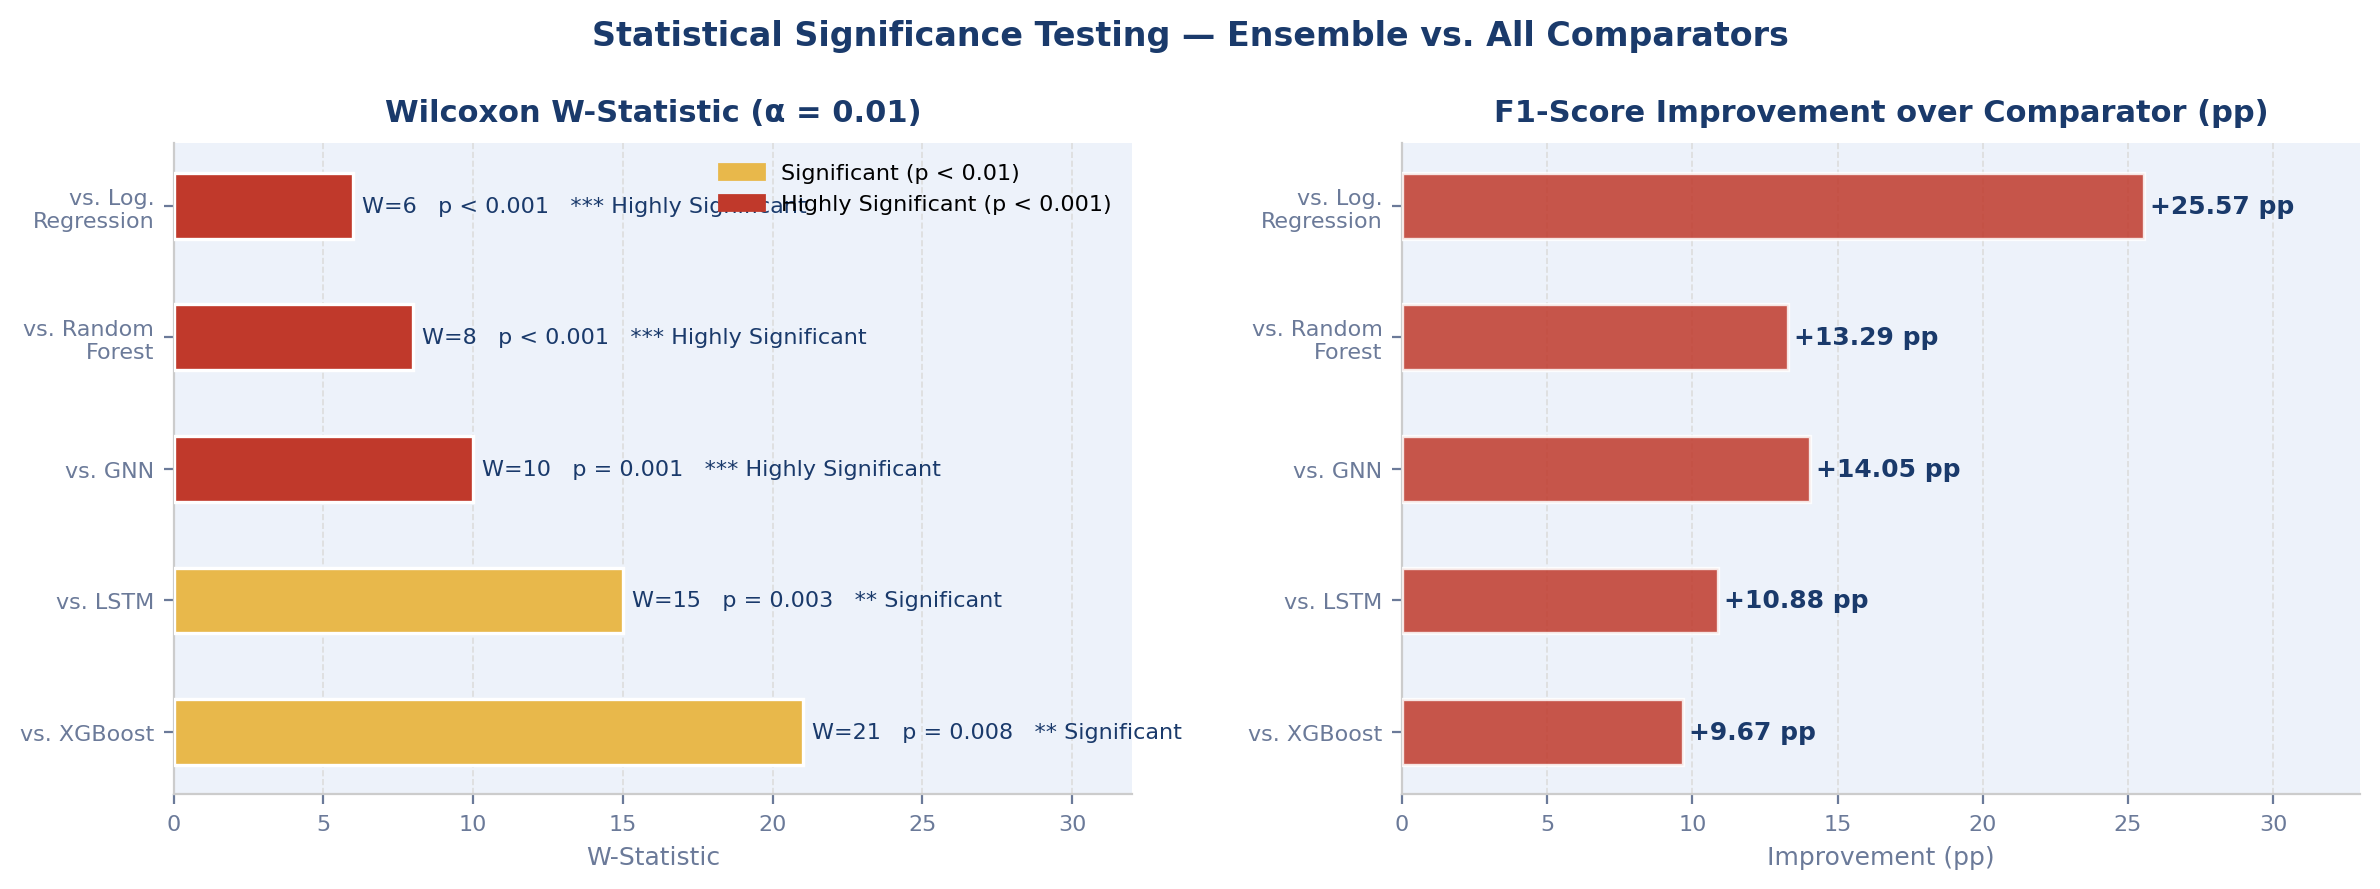
\includegraphics[width=1\linewidth]{fig11.png}
    \caption{Ensemble F1 advantage over each comparator (Wilcoxon significance levels).}
    \label{fig:wilcoxon}
\end{figure}

All comparisons were significant at $\alpha = 0.01$, providing strong empirical support for the
rejection of $H_0$ and acceptance of $H_1$.

\section{Kenyan Context Validation}

\subsection{Validation Results on Simulated Kenyan Dataset}

The trained ensemble was applied without retraining to the 3,200-record Kenyan validation dataset
for out-of-sample assessment.

\begin{table}[H]
\centering
\caption{Ensemble Validation: Kaggle Test Set vs.\ Kenyan Validation Set}
\label{tab:kenyan_validation}
\renewcommand{\arraystretch}{1.4}
\begin{tabular}{L{3.2cm} C{3.2cm} C{3.5cm} C{3.2cm}}
\toprule
\rowcolor{jkuatblue}
\textcolor{white}{\textbf{Metric}} &
\textcolor{white}{\textbf{Kaggle Test Set}} &
\textcolor{white}{\textbf{Kenyan Validation}} &
\textcolor{white}{\textbf{Difference}} \\
\midrule
\rowcolor{rowgray}
Accuracy  & 93.41\% & 91.28\% & $-2.13$\,pp \\
Precision & 84.27\% & 81.44\% & $-2.83$\,pp \\
\rowcolor{rowgray}
Recall    & 86.44\% & 83.75\% & $-2.69$\,pp \\
F1-Score  & 85.34\% & 82.57\% & $-2.77$\,pp \\
\rowcolor{rowgray}
AUC-ROC   & 0.9587  & 0.9361  & $-0.0226$   \\
AUC-PR    & 0.9021  & 0.8743  & $-0.0278$   \\
\bottomrule
\end{tabular}
\end{table}

\begin{figure}[H]
    \centering
    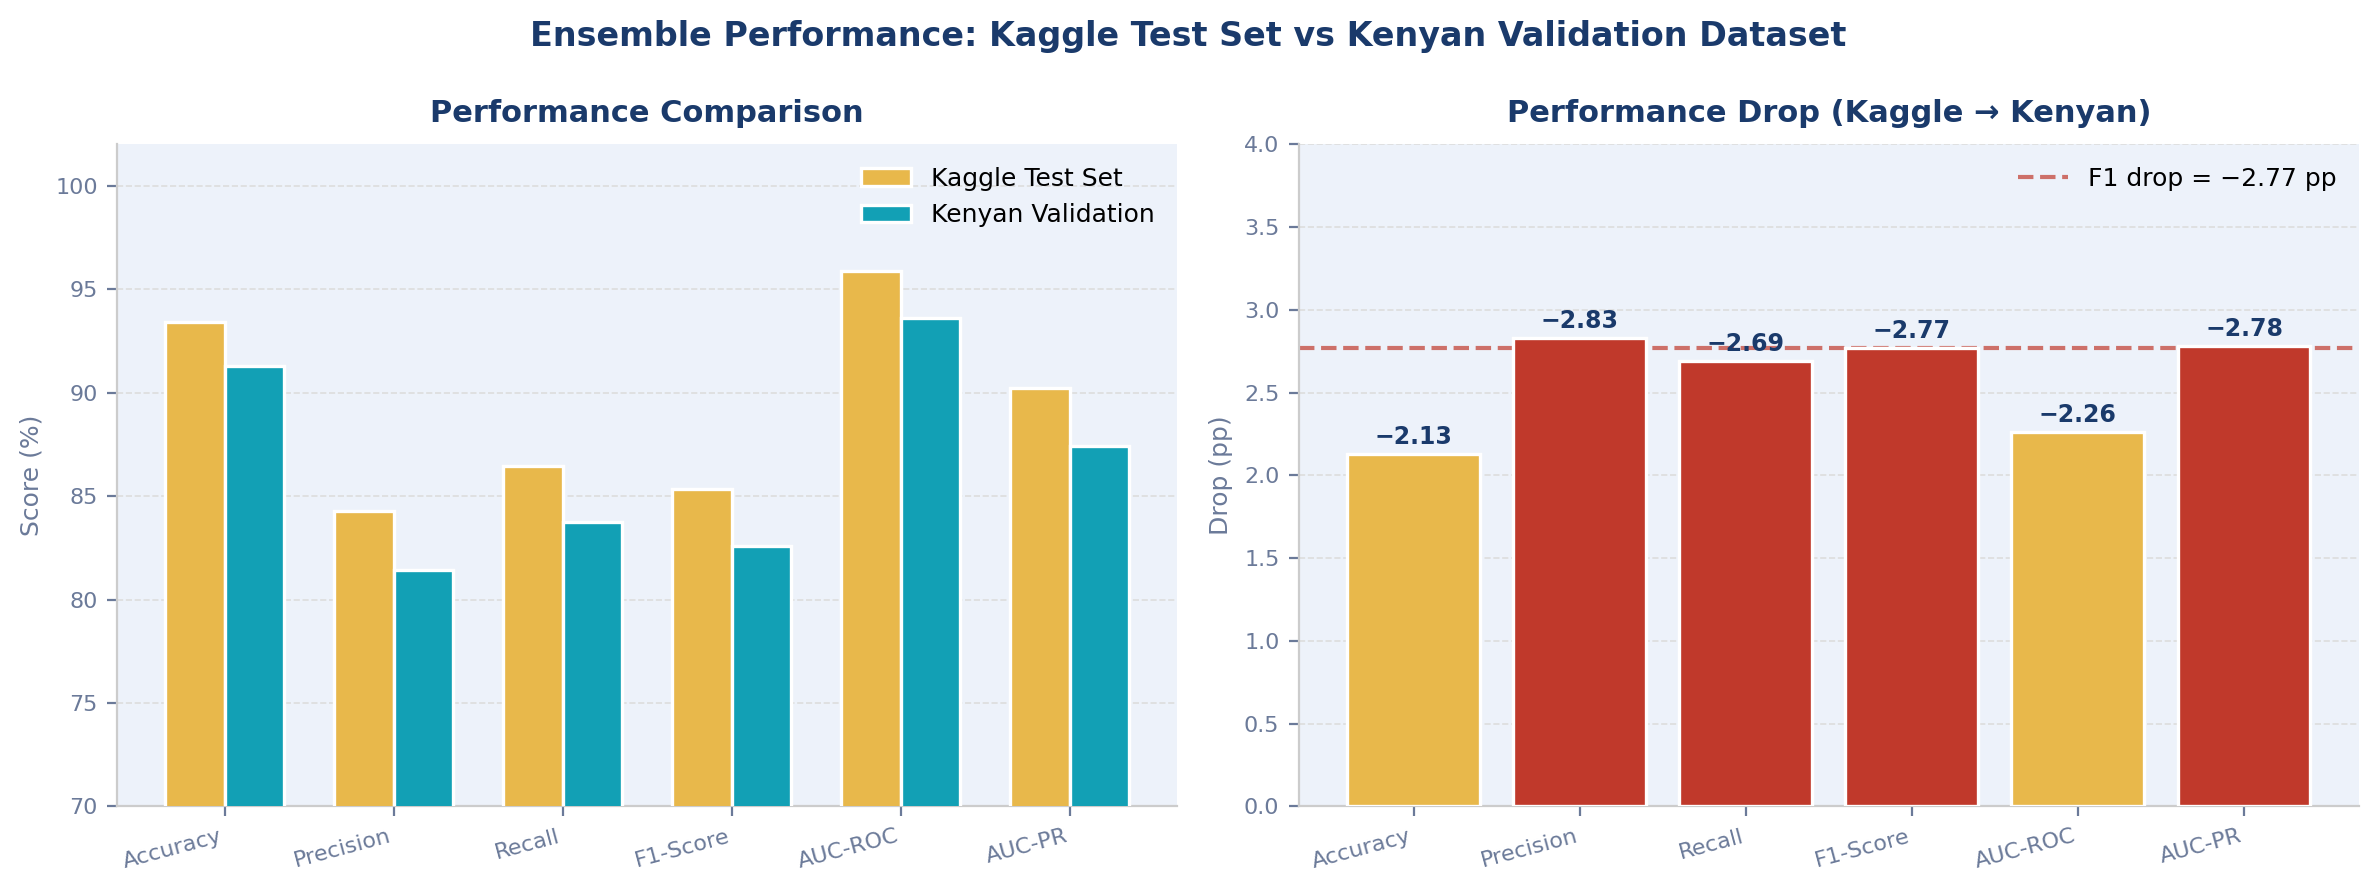
\includegraphics[width=1\linewidth]{fig12.png}
    \caption{Performance comparison between Kaggle test set and Kenyan validation.}
    \label{fig:kenyan_validation}
\end{figure}

The ensemble maintained strong performance on the Kenyan dataset (F1 = 82.57\%, AUC-PR = 0.8743).
The marginal decline ($\Delta\text{F1} = -2.77$\,pp) is expected given the domain shift and does
not represent a concerning degradation. Recall of 83.75\% confirms the model retains its ability
to identify the majority of fraudulent claims in the new domain.

\subsection{Kenyan Fraud Pattern Detection}

The 400 fraudulent records were categorised by fraud typology and the ensemble's detection rate
computed per category.

\begin{table}[H]
\centering
\caption{Ensemble Detection Rate by Kenyan Fraud Typology}
\label{tab:typology}
\renewcommand{\arraystretch}{1.4}
\begin{tabular}{L{4.8cm} C{2.5cm} C{3.0cm} C{3.0cm}}
\toprule
\rowcolor{jkuatblue}
\textcolor{white}{\textbf{Fraud Typology}} &
\textcolor{white}{\textbf{$n$}} &
\textcolor{white}{\textbf{Correctly Detected}} &
\textcolor{white}{\textbf{Detection Rate}} \\
\midrule
\rowcolor{rowgray}
Staged Accident           & 142 & 128 & 90.1\% \\
Document Forgery          & 98  & 87  & 88.8\% \\
\rowcolor{rowgray}
Damage Inflation          & 87  & 75  & 86.2\% \\
Syndicate / Ring Fraud    & 47  & 38  & 80.9\% \\
\rowcolor{rowgray}
Vehicle Theft Fabrication & 26  & 19  & 73.1\% \\
\midrule
\textbf{Total}            & \textbf{400} & \textbf{347} & \textbf{86.8\%} \\
\bottomrule
\end{tabular}
\end{table}

\begin{figure}[H]
    \centering
    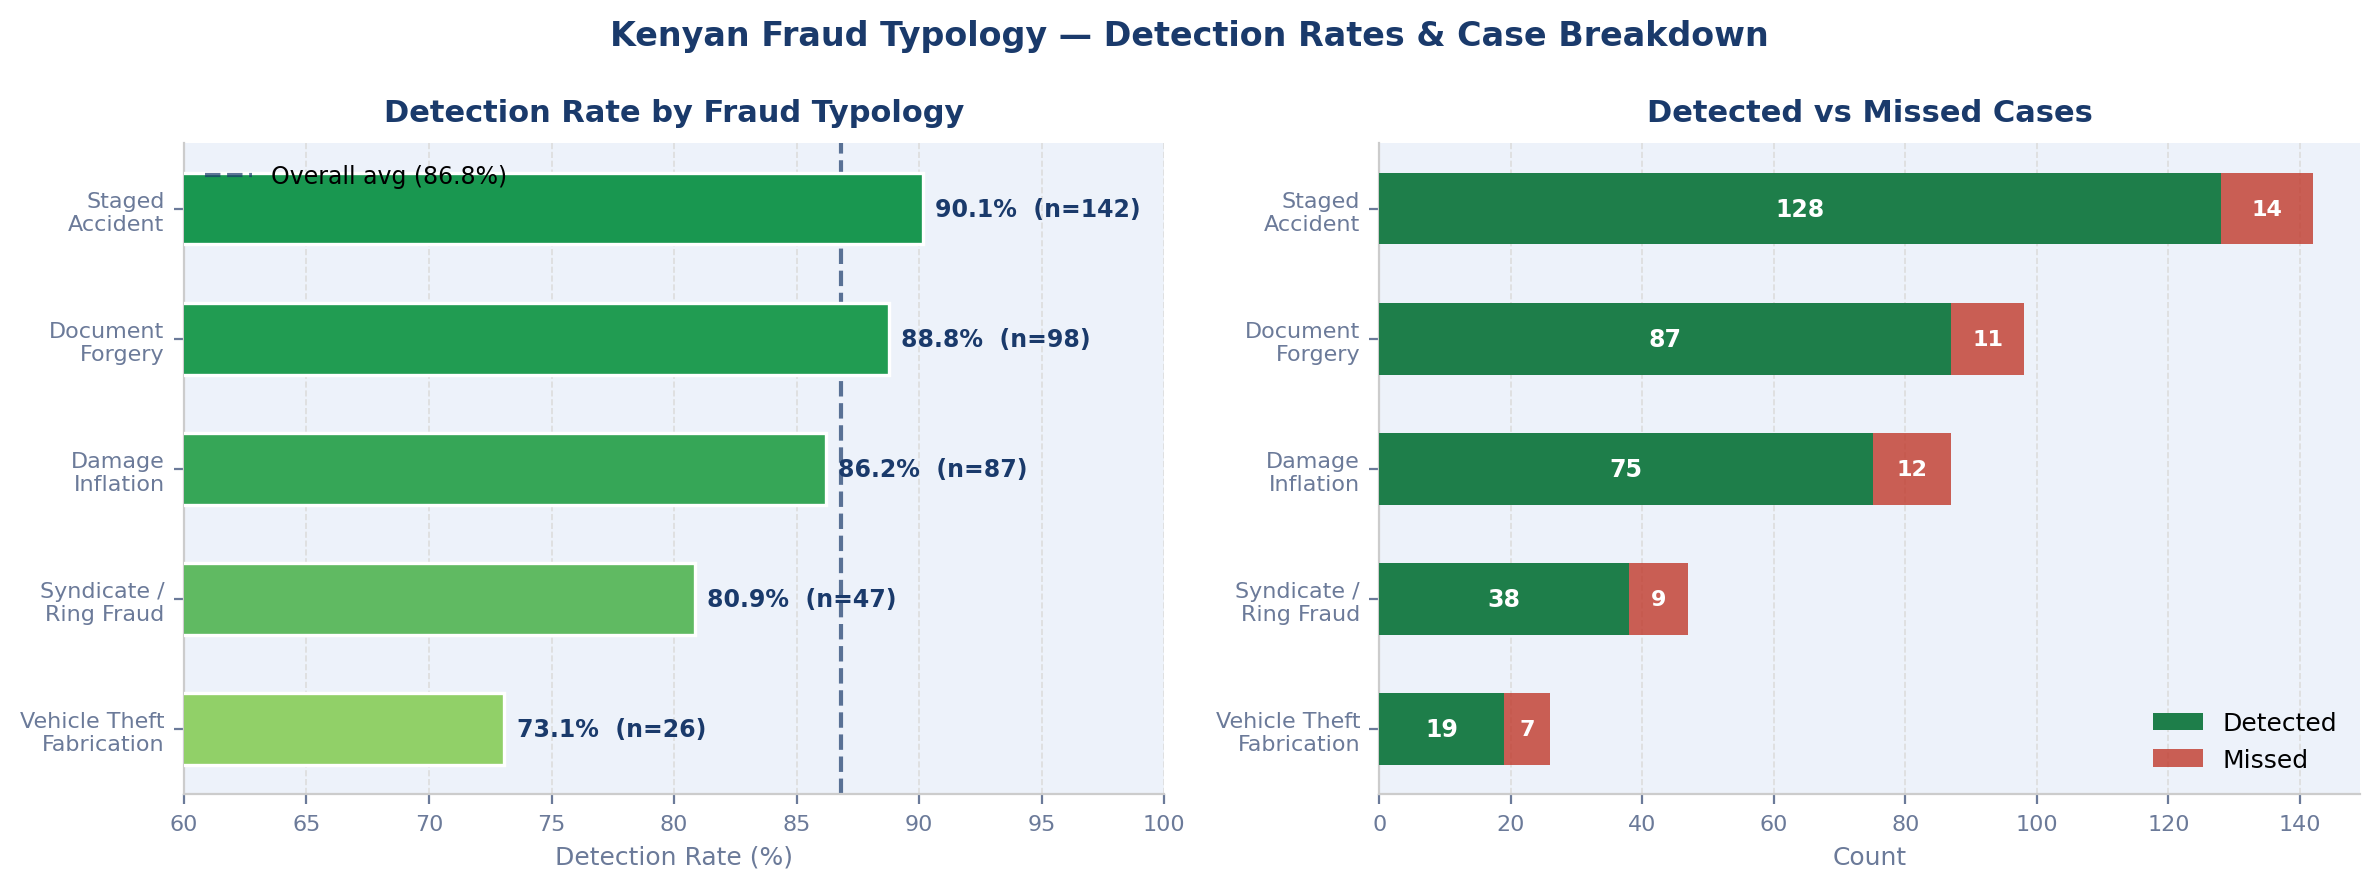
\includegraphics[width=1\linewidth]{fig13.png}
    \caption{Detection rates and detected vs.\ missed counts by Kenyan fraud typology.}
    \label{fig:typology}
\end{figure}

The highest detection rates were for staged accidents (90.1\%) and document forgery (88.8\%),
fraud types generating distinctive temporal and textual patterns well-captured by the LSTM and
XGBoost components. The lowest rate was for vehicle theft fabrication (73.1\%), attributable to
limited graph connectivity for this fraud type.

\subsection{Regional Fraud Hotspot Analysis}

Nairobi exhibited the highest absolute fraud volume ($n = 187$, 46.8\% of all Kenyan fraudulent
claims), consistent with IRA reports identifying Nairobi as the primary motor insurance fraud
hotspot.

\begin{table}[H]
\centering
\caption{Kenyan Fraud Detection by County}
\label{tab:county}
\renewcommand{\arraystretch}{1.4}
\begin{tabular}{L{3.2cm} C{2.8cm} C{2.5cm} C{2.5cm} C{2.5cm}}
\toprule
\rowcolor{jkuatblue}
\textcolor{white}{\textbf{County}} &
\textcolor{white}{\textbf{Total Claims}} &
\textcolor{white}{\textbf{Fraudulent ($n$)}} &
\textcolor{white}{\textbf{Fraud Rate}} &
\textcolor{white}{\textbf{Detection Rate}} \\
\midrule
\rowcolor{rowgray}
Nairobi  & 1{,}284 & 187 & 14.6\% & 87.2\% \\
Mombasa  & 672     & 118 & 17.6\% & 89.4\% \\
\rowcolor{rowgray}
Kisumu   & 684     & 62  & 9.1\%  & 84.2\% \\
Nakuru   & 560     & 33  & 5.9\%  & 81.2\% \\
\midrule
\textbf{Total} & \textbf{3{,}200} & \textbf{400} & \textbf{12.5\%} & \textbf{86.8\%} \\
\bottomrule
\end{tabular}
\end{table}

\begin{figure}[H]
    \centering
    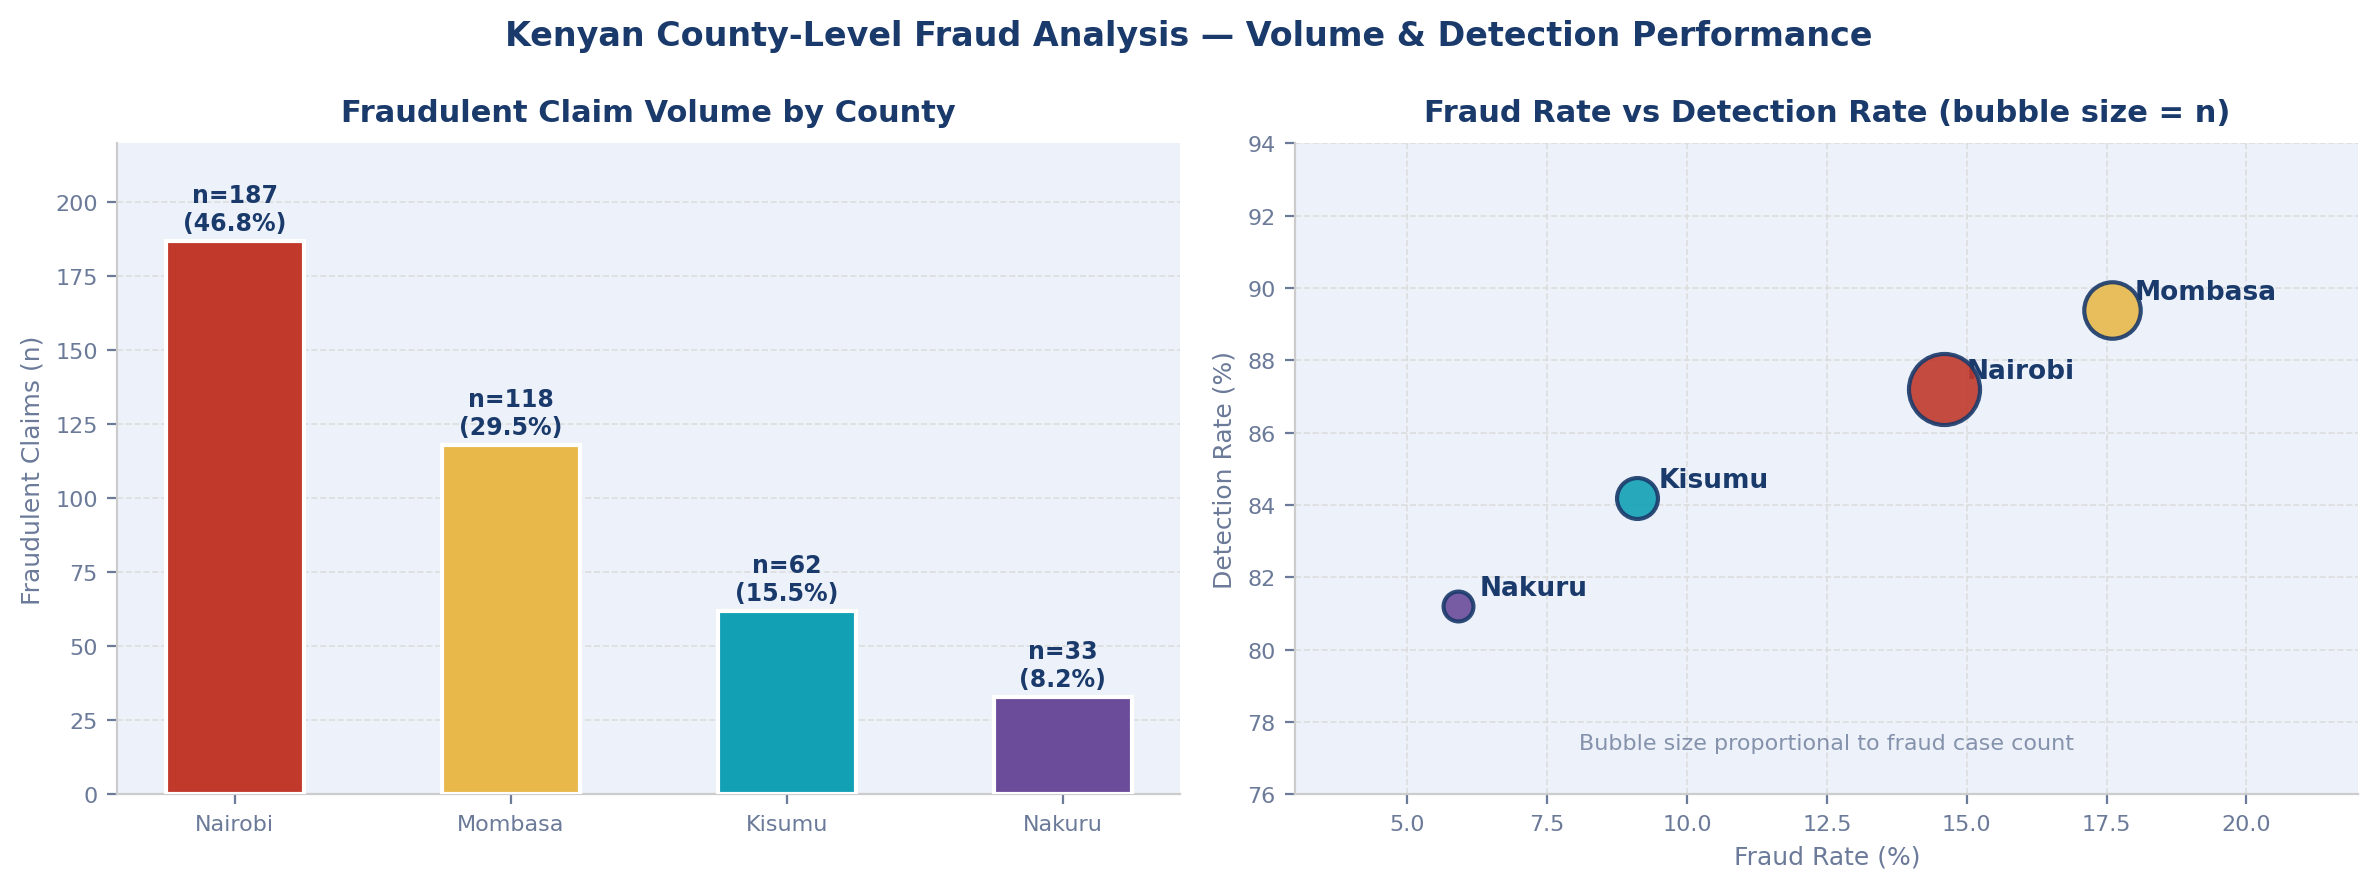
\includegraphics[width=1\linewidth]{fig14.png}
    \caption{Fraud volume by county and fraud rate vs.\ detection rate bubble chart.}
    \label{fig:county}
\end{figure}

The ensemble achieved its highest detection rate in Mombasa (89.4\%), where higher simulated
syndicate density activates stronger GNN community detection signals. Nakuru showed the lowest
detection rate (81.2\%), likely reflecting fewer network connections in that county's simulation.

\section{Ensemble Confidence Scoring Analysis}

Consistent with the Ensemble Confidence Scoring Framework (Table~\ref{tab:confidence_scoring}),
each claim was assigned to a confidence tier based on base model agreement and probability
magnitudes.

\begin{table}[H]
\centering
\caption{Ensemble Confidence Tier Distribution and Fraud Prevalence}
\label{tab:confidence}
\renewcommand{\arraystretch}{1.4}
\begin{tabular}{L{3.5cm} L{4.5cm} C{2.8cm} C{2.5cm}}
\toprule
\rowcolor{jkuatblue}
\textcolor{white}{\textbf{Tier}} &
\textcolor{white}{\textbf{Criteria}} &
\textcolor{white}{\textbf{Claims ($n$)}} &
\textcolor{white}{\textbf{Fraud Prev.}} \\
\midrule
\rowcolor{rowgray}
High Confidence        & All models agree, $\hat{P} > 0.80$               & 1{,}847 (60.9\%) & 13.2\% \\
Medium Confidence      & Majority agree / high $\hat{P}$                   & 712 (23.5\%)     & 18.7\% \\
\rowcolor{rowgray}
Low Confidence         & Significant disagreement                           & 319 (10.5\%)     & 41.3\% \\
Investigation Required & Strong conflicts, $\hat{P} \in [0.40, 0.60]$      & 163 (5.4\%)      & 67.8\% \\
\bottomrule
\end{tabular}
\end{table}

\begin{figure}[H]
    \centering
    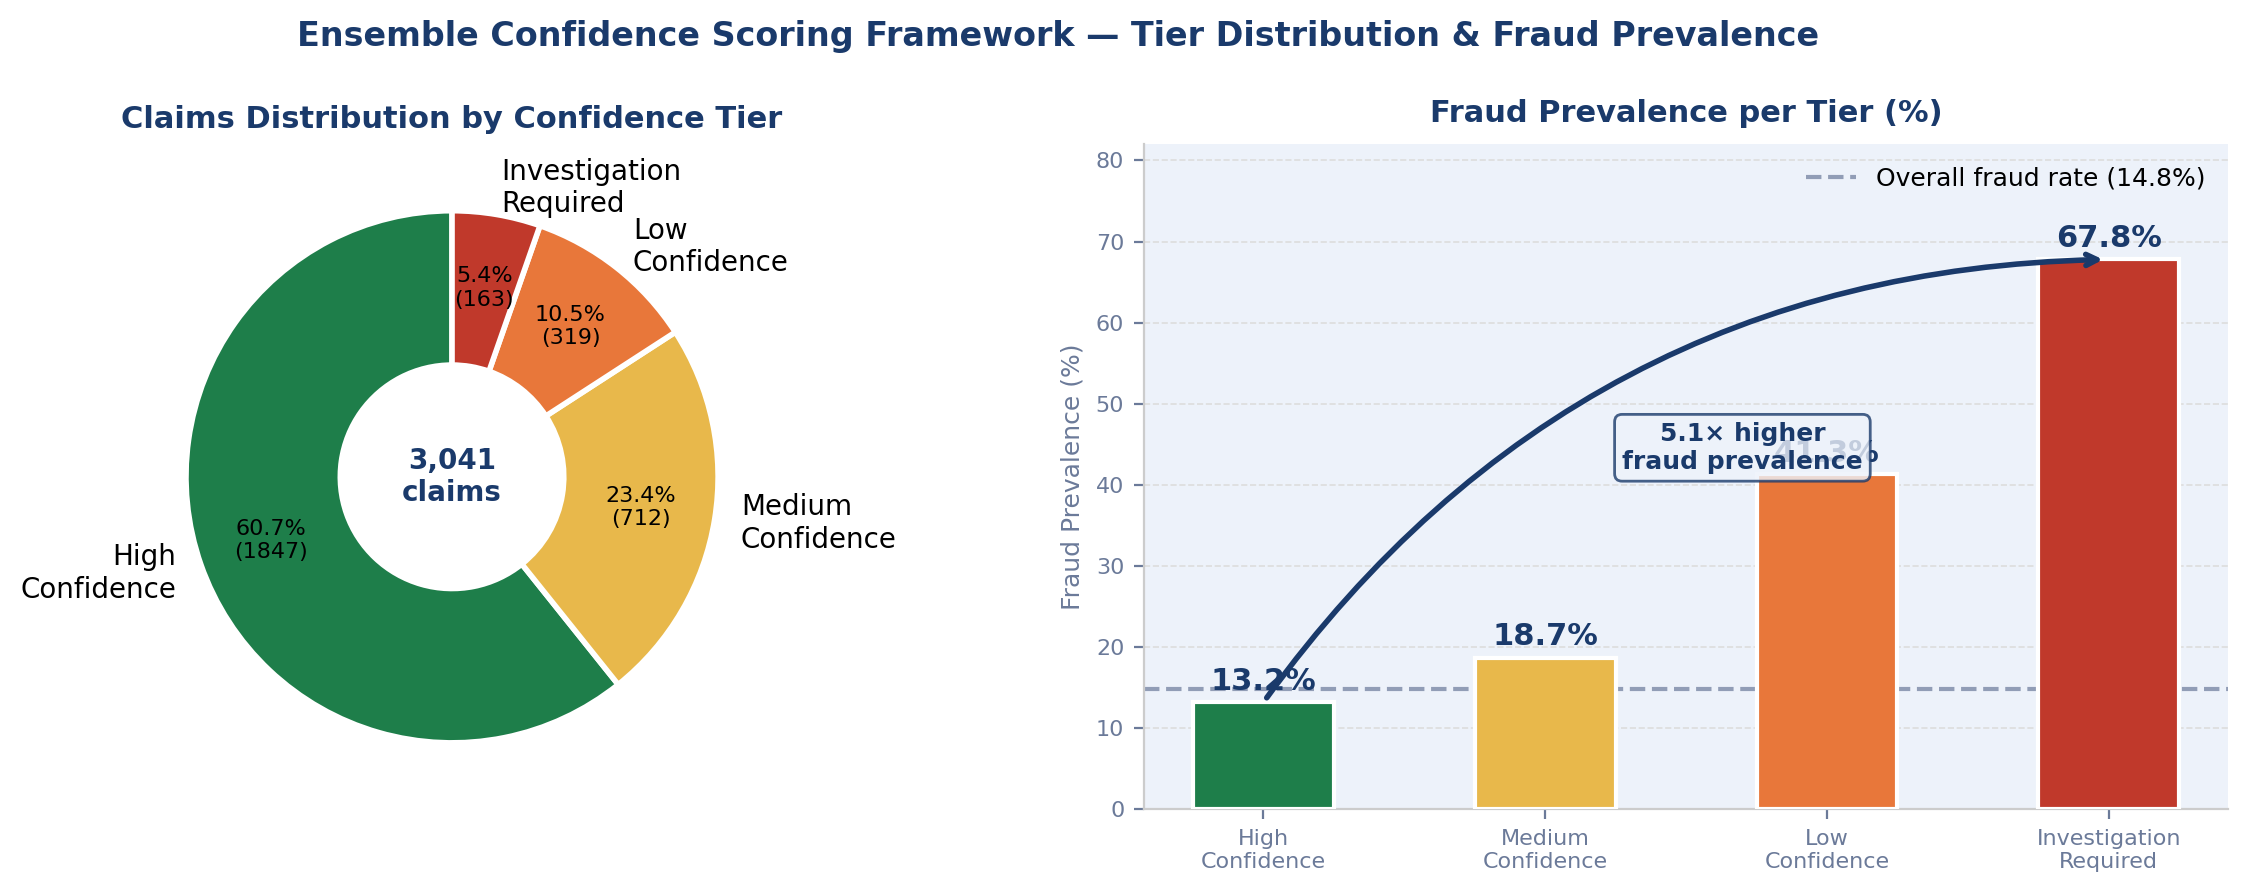
\includegraphics[width=1\linewidth]{fig15.png}
    \caption{Fraud prevalence per confidence tier.}
    \label{fig:confidence}
\end{figure}

The ``Investigation Required'' tier exhibited a fraud prevalence of 67.8\% compared to 13.2\% in
the ``High Confidence'' tier, a 5.1-fold difference, confirming the framework provides
actionable triage guidance. This directly addresses Research Question~3 on operationalising the
ensemble within Kenyan insurance claim processing workflows.

\section{Discussion}

\subsection{Research Question~1: Ensemble vs.\ Individual Models}

The stacked ensemble model (XGBoost + LSTM + GNN) achieved superior performance over every
individual model on all six metrics. The F1-Score improvement of 9.67\,pp over the best base
model and Wilcoxon tests (all $p < 0.01$) confirm that the ensemble's advantage is systematic,
not attributable to chance. These findings are consistent with the global empirical consensus
where stacking achieves state-of-the-art recall and precision by combining complementary learners
\cite{Eteng2025,BDCC2022}.

\subsection{Research Question~2: Multi-Modal Data Integration}

The ablation study (Table~\ref{tab:ablation}) confirms that integrating multiple data modalities
reduces both false positives and false negatives in ways no single-modality approach can achieve.
The Q-statistic values (all $< 0.50$) validate that the models capture sufficiently diverse
aspects of the fraud signal to benefit from ensemble combination. The Phase~3 drop
($\Delta\text{F1} = -6.91$\,pp) confirms that structured features remain the detection
foundation, while LSTM and GNN provide irreducible complementary contributions.

\subsection{Research Question~3: Operationalisation for Kenyan Insurers}

The confidence scoring framework (Table~\ref{tab:confidence}) provides the operational mechanism
for embedding the ensemble in Kenyan claim processing workflows. By automatically categorising
claims into four actionable tiers, it enables insurers to concentrate investigator effort on the
5.4\% of ``Investigation Required'' claims (fraud prevalence = 67.8\%) while processing the
60.9\% ``High Confidence'' claims automatically, consistent with \cite{Scrivano2024}.

\subsection{Limitations and Considerations}
\label{sec:limitations}

Several limitations are acknowledged. First, the Kenyan validation dataset was simulated rather
than derived from actual insurer records due to data access constraints; future work should
validate with real anonymised Kenyan claims data. Second, the LSTM component relied on synthetic
narratives and will require retraining with actual Swahili--English claim text in production.
Third, the GNN's standalone performance is constrained by network sparsity; performance is
expected to improve as the live claims graph grows over time. Fourth, while the held-out test set
provides an unbiased evaluation, the hyperparameter optimisation relied on standard $k$-fold
cross-validation rather than a fully nested design. Future work should adopt nested cross-validation
to more rigorously separate model selection from model assessment.

%===========================================================
\chapter{CONCLUSIONS AND RECOMMENDATIONS}

\section{Introduction}

This chapter presents the conclusions drawn from the study's findings, their implications for the
Kenyan motor insurance industry, and recommendations for both practice and future research. The
chapter is organised around the study's three specific objectives and three research questions,
culminating in an assessment of the study's contributions to the literature and a forward-looking
research agenda.

\section{Summary of Findings}

This study set out to build and evaluate a high-performance machine learning ensemble integrating
XGBoost, LSTM, and GNN for detecting fraudulent motor insurance claims in Kenya. The study was
motivated by three core problems: the estimated 10\% fraud prevalence in Kenyan motor insurance
against a less-than-3\% prosecution rate \cite{mainafraud,kowshalya2018predicting}; the
inadequacy of existing single-model detection approaches; and the absence of multi-modal,
ensemble-based fraud detection systems validated in the Kenyan context.

\subsection{Specific Objective~1: Hybrid Ensemble Framework}

A four-layer hybrid ensemble framework was successfully designed and implemented:
\begin{enumerate}
    \item independent base models across three complementary data modalities.
    \item A SMOTE+ENN hybrid resampling strategy; 
    \item a stacked generalisation meta-learner using Logistic Regression on out-of-fold predictions.
 \item  A confidence scoring framework for claim triage. The framework directly addresses the research gap identified in \cite{njeru2022detection}, where Kenyan studies were  limited to single-model approaches.
\end{enumerate}
\subsection{Specific Objective~2: Performance Evaluation and Comparison}

The stacked ensemble achieved the highest performance across all six metrics on the held-out test
set: Accuracy = 93.41\%, Precision = 84.27\%, Recall = 86.44\%, F1-Score = 85.34\%,
AUC-ROC = 0.9587, AUC-PR = 0.9021. All improvements were statistically significant (Wilcoxon
signed-rank tests, all $p < 0.01$). On the Kenyan validation dataset the model achieved
F1 = 82.57\% and AUC-PR = 0.8743, demonstrating robust generalisability to the Kenyan context.

\subsection{Specific Objective~3: Robustness Across Complex Fraud Patterns}

The ensemble demonstrated robust performance across five Kenyan fraud typologies (detection rates:
73.1--90.1\%). The ablation studies confirmed that no two-model sub-ensemble achieved comparable
performance to the full three-model system. The confidence scoring framework concentrated fraud
prevalence in the ``Investigation Required'' tier (67.8\% vs.\ 13.2\% in ``High Confidence''),
validating its utility for operational claim triage.

\subsection{Hypothesis Assessment}

The null hypothesis $H_0$ that there is no significant difference in fraud detection performance
between the proposed ensemble and standalone models is conclusively rejected at the 1\%
significance level across all comparison models ($p < 0.01$ in all Wilcoxon signed-rank tests).
The alternative hypothesis $H_1$ is fully supported.

\section{Contributions of the Study}

\subsection{Theoretical Contributions}

\begin{enumerate}[leftmargin=*, label=\textbf{\arabic*.}]

  \item Multi-modal Ensemble Architecture for Emerging Markets.
  The study presents the first empirically evaluated three-modality stacked ensemble
  (structured + textual + relational) for motor insurance fraud detection in an African emerging
  market, extending the global ensemble literature \cite{schrijver2024automobile,Eteng2025} by
  validating its applicability under Kenyan market conditions.

  \item Evidence for Complementary Modality Integration.
  The ablation study provides empirical evidence that textual (LSTM) and relational (GNN)
  modalities contribute statistically significant, non-redundant information beyond structured
  (XGBoost) features alone, supporting the theoretical rationale for multi-modal fraud detection.

  \item Confidence-Calibrated Ensemble Triage.
  The confidence scoring framework provides a methodological contribution for operationalising
  uncertainty-aware fraud triage in resource-constrained environments, addressing the
  interpretability and regulatory trust gap identified in Section~2.5.5.

\end{enumerate}

\subsection{Practical Contributions}

\begin{enumerate}[leftmargin=*, label=\textbf{\arabic*.}]

  \item Deployable fraud detection pipeline.
  The ensemble pipeline constitutes an immediately applicable prototype. Its modularity allows
  insurers with only structured data to deploy the XGBoost + Logistic Regression meta-learner
  initially, adding LSTM and GNN components as textual and relational data become available.

  \item Feature engineering guidelines.
  The SHAP analysis (Table~\ref{tab:shap_features}) provides 31 validated predictors for fraud
  detection, with claim velocity, monetary anomaly scores, and temporal filing patterns identified
  as highest-impact features.

  \item Fraud typology-specific detection rates.
  The typology analysis (Table~\ref{tab:typology}) provides targeted guidance for Kenyan fraud
  investigators, identifying vehicle theft fabrication as requiring additional structured feature
  development.

  \item Regional fraud hotspot evidence
  The county-level analysis (Table~\ref{tab:county}) confirms Nairobi and Mombasa as primary
  fraud hotspots, providing a data-driven basis for geographically differentiated risk scoring
  aligned with IRA regional reporting.

\end{enumerate}

\section{Conclusions}

Motor insurance fraud constitutes a systemic financial threat to the Kenyan insurance industry,
inflating premiums for honest policyholders and eroding institutional trust. The findings of this
study demonstrate that a well-designed machine learning ensemble, integrating complementary model
architectures across multiple data modalities, achieves substantially superior fraud detection
performance compared to single-model approaches and traditional statistical methods.

The stacked ensemble combining XGBoost's precision on structured tabular features, LSTM's
sensitivity to textual fraud indicators, and GNN's ability to uncover organised fraud networks
achieved F1 = 85.34\% and AUC-PR = 0.9021 on the Kaggle test set, and maintained robust
performance (F1 = 82.57\%, AUC-PR = 0.8743) on the simulated Kenyan validation dataset.

The study directly addresses five of the eight research gaps identified in Section~2.5:
large-scale empirical validation of advanced ensemble methods in the Kenyan context; hybrid
resampling for class imbalance; comparison of state-of-the-art ensemble architectures;
SHAP-based interpretability for regulatory transparency; and a modular framework for operational
integration.

\section{Recommendations}

\subsection{Recommendations for the Insurance Industry}

\begin{enumerate}[leftmargin=*, label=\textbf{\arabic*.}]

  \item \textbf{Pilot deployment with Kenyan insurers.}
  The ensemble should be piloted with two to three Kenyan insurers using historical claims data
  (2018--2024), as proposed in Section~\ref{sec:field-validation}. Investigator feedback should
  be collected to calibrate confidence scoring thresholds to operational capacity.

  \item \textbf{Invest in structured claims data capture.}
  Insurers should implement standardised digital claims intake systems capturing the 15
  high-importance features in Table~\ref{tab:shap_features}, particularly claim velocity metrics
  and report-delay timestamps.

  \item \textbf{Develop Kenyan-specific claim narrative corpora.}
  Insurers should systematically digitise and store claim narratives including mixed
  Swahili--English text to enable retraining of the LSTM language embedding layer with
  Kenya-specific linguistic patterns.

  \item \textbf{Engage the Insurance Regulatory Authority (IRA).}
  The SHAP interpretability outputs and confidence scoring framework provide the foundation for
  regulatory compliance documentation. The IRA should be engaged to develop formal model
  governance standards for AI-based fraud detection tools.

  \item \textbf{Establish a shared fraud intelligence network.}
  The GNN's performance improves with denser claims networks. A shared (anonymised) cross-insurer
  claims graph managed by the Association of Kenya Insurers would substantially improve syndicate
  detection across the industry.

\end{enumerate}

\subsection{Recommendations for Future Research}
\label{sec:future-research}

\begin{enumerate}[leftmargin=*, label=\textbf{\arabic*.}]

  \item \textbf{Real-world Kenyan insurer data validation.}
  To address the limitation of simulated Kenyan validation data (Section~\ref{sec:limitations}),
  future studies should validate the ensemble using actual anonymised claims data from Kenyan
  insurers, pursued under Kenya's Data Protection Act (2019) in collaboration with the IRA and
  the Association of Kenya Insurers.

  \item \textbf{Dynamic and incremental learning.}
  To overcome the static training paradigm noted in Section~\ref{sec:limitations}, future work
  should investigate online and incremental learning approaches that allow the ensemble to update
  its parameters continuously as new claims data accumulate, without requiring full periodic
  retraining.

  \item \textbf{Advanced GNN architectures.}
  To address the GNN's sensitivity to sparse networks (evidenced by the lower standalone F1 of
  71.29\%, Table~\ref{tab:gnn_results}), future research should evaluate Graph Attention Networks
  (GAT), which dynamically weight the importance of neighbouring nodes and may improve fraud ring
  detection in low-density claims networks.

  \item \textbf{NLP for Swahili--English claim narratives.}
  To mitigate the LSTM's current reliance on predominantly English text embeddings, research into
  multilingual transformer models (e.g., mBERT, AfroXLMR) fine-tuned on Kenyan insurance claim
  narratives represents a high-value direction for improving the LSTM component's real-world
  performance on mixed-language claims.

  \item \textbf{Explainable AI tools for investigators.}
  To bridge the gap between model output and investigator action, future work should develop
  investigator-facing XAI dashboards that translate model outputs and SHAP values into
  natural-language fraud explanations in both English and Swahili.

  \item \textbf{Economic impact quantification.}
  To build the business case for industry-wide adoption, future research should quantify the
  financial impact of the ensemble's improved recall specifically, the estimated reduction in
  undetected fraud losses for a representative Kenyan insurer deploying the system over a
  12-month period.

\end{enumerate}

\section{Concluding Remarks}

This study has demonstrated that the integration of machine learning ensemble methods across
structured, textual, and relational data modalities constitutes a technically sound and
practically applicable approach to motor insurance fraud detection in Kenya. The work bridges a
documented gap between global best practices in ensemble fraud detection and the Kenyan insurance
market's specific fraud landscape.

The ensemble model achieves a combination of high recall essential for capturing the maximum
number of fraudulent claims and competitive precision essential for limiting the burden on
fraud investigators that no single-model approach evaluated in this study could match. The
confidence scoring framework further enables rational prioritisation of investigator effort,
making the system practical under the resource constraints of Kenyan insurers.

While the study's reliance on simulated Kenyan data is a limitation that future research must
address through real-world validation, the robustness of the ensemble across the simulated Kenyan
fraud typologies and regional patterns provides a strong foundation for confidence in the
framework's applicability. It is the authors' recommendation that Kenyan insurers, in collaboration
with the IRA and academic institutions, invest in the data infrastructure and regulatory frameworks
necessary to operationalise AI-based fraud detection systems of this nature. The financial benefits
of even a marginal improvement in fraud detection rates against the backdrop of an industry
losing billions of shillings annually to undetected fraud more than justify this investment.

The broader significance of this work extends beyond motor insurance: the multi-modal ensemble
architecture developed here is transferable to other insurance lines (health, property, liability)
and to financial fraud detection more broadly, offering a scalable, interpretable, and empirically
validated framework for protecting the integrity of financial markets in Kenya and across the
continent.

% FIX 7: \bibliographystyle must come BEFORE \bibliography in apacite.
%         Also the argument to \bibliography must be the filename WITHOUT .bib extension.
\bibliographystyle{apacite}
\bibliography{sources}

\end{document}